\documentclass{book}
\usepackage{a4wide,amsthm,parskip,graphicx,amsfonts,algo,gensymb,tabularx,fancyvrb,tikz,amsmath,generic,stmaryrd,dsfont,pgf-umlsd,floatflt,fancyhdr,comment}
\usepackage[pdftex,pdfstartview=FitV]{hyperref}
\usepackage[english]{babel}
\usetikzlibrary{arrows}
\usetikzlibrary{shapes.multipart}
\hypersetup{
        pdftitle={Design and verification of the SmartPixel II protocol},
        pdfauthor={Rink Springer},
        pdfkeywords={smartpixel mcrl2}
}


\pagestyle{fancy}
\fancyhf{}
\fancyhead[LE,RO]{\bfseries\thepage}
\fancyhead[LO]{\bfseries\rightmark}
\fancyhead[RE]{\bfseries\leftmark}
\renewcommand{\headrulewidth}{0.5pt}
\renewcommand{\footrulewidth}{0pt}
\addtolength{\headheight}{0.5pt}
\fancypagestyle{plain}{%
        \fancyhead{}
        \renewcommand{\headrulewidth}{0pt}
}

\title{Design and verification of the SmartPixel II protocol}
\author{Rink Springer}

\begin{document}

\begin{titlepage}
\hfill Eindhoven, \today
\null\vfill
\vspace{20mm}
\begin{center}\Large
\hspace{2cm}Design and verification \par
\hspace{2cm} of the \par
\hspace{2cm}SmartPixel II protocol\vskip1cm
\hspace{2cm}\normalsize by \par \hspace{2cm}Rink P. W. Springer
\vskip3cm
\hspace{2cm}in partial fulfillment of the requirements for the degree of\par
\vskip5mm
\hspace{2cm}\textbf{Master of Science}\par
\hspace{2cm}\textbf{in Computer Science and Engineering}
\vskip3cm
\end{center}\vfill
Supervisor:\\
M. A. Reniers, TU/e department of Mathematics and Computer Science\\
W. Hendriksen, Devlab \\
\end{titlepage}

\frontmatter

\chapter{Preface}
\index{preface}

This report will describe my graduation internship at Philips Research in Eindhoven. It is written in an informative manner, with the exception of my personal evaluation which, of course, can't be objective or purely informative. The report is written using the guidelines as outlined in \cite{ROR}.

The goal of the internship was to design and implement a real time filesystem for Linux. This is illustrated further in the project description on page \pageref{project}.

The target audience is mostly people having an interest in the process or the execution of my internship. The technical documentation of the project is a separate document, which is included as appendix A. The project management plan, or \emph{plan van aanpak}, is included as appendix B.

Finally, I'd like to to thank the following people who helped me during my internship: Bas van Tiel, Michiel van Slobbe, Ron Eringa, Ad Denissen, Mischa Geldermans, Christ Vriens, Werner Almesberger and Wim Zijlmans.

Rink Springer \\
May 2005

\section*{Acknowledgments}

First and foremost, this thesis would not be its current form without the help of my supervisor, Michel Reniers. We regularly discussed the current results and reflected upon the status of the work, which both have really aided me during this project. I would also like to thank Simon Janssen for the useful discussions and constructive criticism while performing the project, as well as all other persons who have read my thesis and provided useful comments. Last but not least, the mCRL2 development team has been very responsive in regard to my bug reports - I would especially like to thank Jeroen van der Wulp for his patience and help.

\vspace{5mm}
\begin{tabularx}{\textwidth}{Xr}
 & Eindhoven, July 2008 \\
 & Rink Springer \\
\end{tabularx}

\chapter*{Abstract}

The SmartPixel system consists of a set of independent nodes, which have to cooperate in order to accomplish desired functionality. This makes the system a good example of a completely distributed system: all nodes have to work together to achieve the intended result. The result is that the SmartPixel system is very well suited for a detailed analysis.

In the thesis, we will first present the SmartPixel system and provide an introduction to the process theory used. From then on, the different phases of the system will be individually modeled and validated, after which the focus will be on the system as a whole. The remainder of the thesis will attempt to transform timed models to untimed models in an attempt to prove more properties of the system. Finally, the findings are summarized in the concluding words.


\tableofcontents

\mainmatter

\chapter{Introduction}
\index{introduction}

This technical report describes the LIMEFS filesystem. This filesystem was written during my graduation project of my Computer Sciences study at Fontys Hogescholen in Eindhoven and carried out at Philips Research in Eindhoven. The goal was design and implement a framework for realtime file storage, which came down to implementing a realtime filesystem which can provide guaranteed I/O performance.

The report will provide a rough description of the Linux Virtual File System structure. The next part will focus completely on the design and implementation of the XXFS filesystem, followed by concluding statements on the project.

\chapter{Overview}
\label{sec:overview}

% Wat zijn die smartpixel dingen?
% hoe ziet een netwerk eruit?
% wat moeten ze doen?

A single \emph{SmartPixel} is a square device, which contains a light that can be switched on or off. The device also contains four physical connectors, referred to as $0, \dots, 3$, which reside on each side and are used in order to communicate with a neighboring SmartPixel. A number of these SmartPixels connected together form a network. We shall refer to a single SmartPixel in such a network as a \emph{node}. It is important to note that all nodes contain completely identical hardware and software; the only property that makes them distinguishable is an \emph{identification number}, or \emph{id}, which is unique per node. Since the nodes are square-sized, they can be rotated any multiple of $90 \degree$ before they are connected to adjacent nodes. Nodes know nothing of their position in the network, let alone whether each side has a neighbor - all they can do is send messages to adjacent neighboring nodes, receive messages from such nodes and switch the light on or off. A visual representation of such a SmartPixel can be found in Figure \ref{fig:smartpixel}.

\begin{figure}[h]
 \centering
 \begin{tikzpicture}
  \draw[<-,>= stealth'] (1.75,1) -- (1.75,0);
  \draw[->,>= stealth'] (2.25,1) -- (2.25,0);
  \draw[->,>= stealth'] (1.75,3) -- (1.75,4);
  \draw[<-,>= stealth'] (2.25,3) -- (2.25,4);
  \draw[<-,>= stealth'] (0,1.75) -- (1,1.75);
  \draw[->,>= stealth'] (0,2.25) -- (1,2.25);
  \draw[<-,>= stealth'] (3,1.75) -- (4,1.75);
  \draw[->,>= stealth'] (3,2.25) -- (4,2.25);
  \draw (1,1) rectangle (3,3);
  \draw (2,2) circle (0.45cm);
 \end{tikzpicture}
 \caption{\label{fig:smartpixel} Visual representation of a single SmartPixel}
\end{figure}

Once such a network of nodes has been assembled, connected and switched on, the nodes will perform some necessary initialization steps in order to determine the network configuration; these steps are outlined in Section \ref{sec:operation}. Once the initialization is completed, the nodes continue to perform their main function: display the first figure out of a list of figures, delay a few seconds, display the next figure, delay a few seconds, etc. This keeps going until we pull the plug. If nodes are physically altered, such as by adding or removing nodes while the system is operating, the system should adapt to the new situation. For the purposes of these figures, it is assumed that the network itself is square-sized, $N \times N$ nodes. A possible configuration is presented in Figure \ref{fig:examplenet}: each square is a node, where the $0$, $1$, $2$, $3$ denote the north, east, south and west connections of this node. Finally, the number represents the unique identification number of the node.

\begin{figure}[h]
\centering
\begin{nodefigure}
\nodegrid{4}{0}{0}{0/0/ 8/$0$/$1$/$2$/$3$, 1/0/12/$2$/$3$/$0$/$1$,
                   2/0/11/$3$/$0$/$1$/$2$, 3/0/ 4/$2$/$3$/$0$/$1$,
                   0/1/15/$1$/$2$/$3$/$0$, 1/1/ 1/$0$/$1$/$2$/$3$,
                   2/1/ 6/$1$/$2$/$3$/$0$, 3/1/ 7/$1$/$2$/$3$/$0$,
                   0/2/ 5/$0$/$1$/$2$/$3$, 1/2/10/$0$/$1$/$2$/$3$,
                   2/2/ 3/$3$/$0$/$1$/$2$, 3/2/13/$1$/$2$/$3$/$0$,
                   0/3/ 9/$1$/$2$/$3$/$0$, 1/3/14/$0$/$1$/$2$/$3$,
                   2/3/16/$3$/$0$/$1$/$2$, 3/3/ 2/$0$/$1$/$2$/$3$}
\end{nodefigure}
\caption{\label{fig:examplenet} Example of a $4 \times 4$ network of SmartPixel nodes}
\end{figure}

While the usefulness of such a system can be doubted, the interesting challenges that will arise while specifying and proving a model cannot. How will nodes know `what to do'? How can we ensure that the system remains as operational as possible whenever some nodes fail? Will the algorithms proposed in Section \ref{sec:operation} turn out to be correct, or will unforeseen side-effects show up in the model? 

\section{Hardware}
\label{sec:hardware}

The hardware in use consists of a PCB board of $3 \times 3$ cm, containing an ATMega644 microcontroller and some assorted parts. A message can be sent out to each of the four directions individually and it is possible to tell from which direction a message was received. In each direction, only a single message can be sent at a time; these messages are transmitted using Manchester encoding. While a message is being sent, an incoming message will still be received.

\section{Assumptions}
\label{sec:assumptions}

Considering the hardware and requirements of the system, this design is based on the following assumptions:

\begin{enumerate}
\item \label{ass:diffspeed} Each node may have a slight clock speed deviation \\
There may be a slight deviation ($\pm 10\%$) from the specified clock speed - this deviation is unknown to the node.
%\item \label{ass:reliablemsg} Messages always arrive, there are no resends needed \\
%The assumption is that the encoding in use will detect corruption and request resends as needed.
\item \label{ass:alternodes} Nodes can be added, removed and switched on/off at any time in the system.
\item \label{ass:speedymsg} The delay between node $A$ transmitting a message and node $B$ receiving it is negligible.
\item \label{ass:corruptmsg} It is possible to distinguish between a valid and corrupt message. \\
We will only consider retrieving valid messages; corrupt messages will always be discarded.
\end{enumerate}

\chapter{Introduction to process algebra}

% wat is een actie? wat is een proces? communicatie.

\section{Basics of process algebras}
\label{sec:pabasics}

The foundation of the formal modeling methodology as used throughout the thesis is known as \emph{process algebra}: a process algebra is an abstract method to describe the behavior of a system from a high-level perspective. The process algebra used in the thesis is the one used by mCRL2 \cite{groote07mcrl2} as described in \cite{groote07radv}, which in turn is based on ACP \cite{bergstra84acp}. Process algebras are specified using axioms; axioms can be seen as rules which are always valid. All axioms are presented in Appendix \ref{apx:axioms}.

Generally, a system is divided into a number of \emph{processes}. The idea of this division is that processes are independent: they only influence each other when explicitly modeled that they do, by means of communication (this will be discussed in Section \ref{sec:macomm}). Of course, these processes need to work together to hopefully achieve the desired effect. We refer to the set of all processes as the \emph{system} we are modeling. For example, if we were to model a coffee vending machine, there may be a process $\mathcal{U}$ responsible for the user input, a process $\mathcal{P}$ responsible for handling payment and a process $\mathcal{S}$ responsible for serving the coffee. If money has been inserted, the payment process should inform the user interface, to allow the user to see how much money has been inserted into the machine. Likewise, if a flavor has been selected and enough money has been inserted into the machine, the serving process should be instructed to start brewing coffee.

In the example above, the overall coffee vending system consists of processes $\mathcal{U}$, $\mathcal{P}$ and $\mathcal{S}$, which all run in parallel. As these processes run in parallel, it is possible to combine them into a single process yielding the same behavior as all processes in parallel would, by means of the \emph{parallel operator} $\parallel$. The result is that we can obtain a process $\mathcal{M}$ illustrating the behavior of the entire coffee vending machine, for which it holds that $\mathcal{M} = \mathcal{U} \parallel \mathcal{P} \parallel \mathcal{S}$. This operator will be covered in Section \ref{ref:parallelop} - for now, the most important notion is the existence of the operator.

\section{Actions}
\label{sec:actions}

Modeling can generally be regarded as describing a system from a high-level perspective: most implementation details, for example the precise steps required to communicate a message from one system to another are not discussed: such implementation details are rarely interesting from such a high-level abstraction. This brings us to the notion of \emph{actions}: basically, an action is an atomic event which may or may not occur - for example, we may have an action $opendoor$, which illustrates that some door has been opened and an action $closedoor$ which illustrated the same door has been closed. It must be noted that a system designer is always free to chose the action names; claiming action $a$ illustrates that some door has been opened is fine as well. To this end, an overview mapping each action to an atomic event should always be included in every model to prevent possibly confusion or ambiguity. For the remainder of this chapter, we shall use action names $a$, $b$, $c$, etc. if we need to refer to some arbitrary action without a special function.

One may wonder, since we appear to only support actions, how events are being represented within our formalism. This introduces some food for thought: what is the difference between an action and an event? A natural response is that an action represents a change initiated by the process, whereas an event represents a change initiated by the environment. Yet, this distinction is actually confusing, since if we were to create a model detailing the interactions between two processes, a change initiated by the first process would be an environment change for the second process, and the other way around! From this, it follows that distinguishing between actions and events is not a very good idea: it makes matters much more confusing.

Based on the reasoning above, any atomic event can be encoded as an action, like opening/closing doors, but there could be an event $isDoorOpen$, which indicates a door is sufficiently opened to allow a person to move through it. If we want to check whether the door is sufficiently opened, we attempt to issue a $isDoorOpen$ action. If this is possible, the door is indeed sufficiently opened. If this action cannot be performed (this is referred to as an action being \emph{blocked}), we know the door is not sufficiently opened.

Given this notion of actions, we note that we may want to parametrize actions: if we are modeling communication of numbers, we do not want to introduce action $send\emph{0}$ to indicate we have sent a $0$, $send\emph{1}$ for sending a $1$, etc - we simply issue a $send(0)$, $send(1)$ and so forth, and define $send : \mathds{N}$: an action that takes a natural number as parameter. Of course, we can also use multiple parameters: if we have $send : \mathds{N} \times \mathds{B}$, this indicates action $send$ takes a natural number and a boolean value.

There is an important special action, the \emph{deadlock} action $\delta$, which illustrates that no action can be done and that there is no termination possible; once a process is in a deadlock state, it cannot do anything and will stay deadlocked forever. While it may seem a bit odd to introduce the notion of a deadlock in our model, it is generally not directly used within specifications but rather the result of other operators, the most important of which will be introduced in the next sections. The $\delta$ action has two distinct properties: if we can chose between a deadlock or another action, the other action will always be selected; this makes sense as we intend to avoid a deadlock as long as possible. Secondly, we cannot continue after a deadlock: the process is deadlocked, so there is nothing it can do. These properties are illustrated in axioms A6 and A7 (the precise meanings of $+$ and $\cdot$ will be illustrated in Section \ref{sec:specifyproc})

\section{Multi-actions and communication}
\label{sec:macomm}

As we are modeling independent systems, it may be possible that multiple atomic actions are performed at exactly the same moment in time. This is denotes as $a \comm b \comm \dots$: actions $a$, $b$, etc. all occur at exactly the same moment in time. While this may seem odd at first, remember that systems generally consist of multiple processes, and these processes are all independent so they can issue an action regardless of what another process is doing.

Using this concept of multi-actions, we can introduce the notion of \emph{communication}: if one process performs a $send(1)$ action to indicate it sends the value $1$, we want another process to be able to perform a $receive(1)$ action (but not $receive(2)$ for example, as value $2$ clearly is not sent). This means we have to specify that actions $send$ and $receive$ in a sense `belong' together: we want to combine them in a single action. This is achieved using the concept of a \emph{communication operator}, which we call $\Gamma_C$: this $\Gamma_C$ maps a multi-action to a new action, using the definitions as supplied in the set $C$. For example, we would define $C = \{ send \comm receive \rightarrow communicate \}$ to illustrate that we refer to a $send$ action simultaneously occurring with a $receive$ action as a $communicate$ action. This means that if we apply communication set $C$ to multi-action $send \comm receive$, we expect to obtain $communicate$, which is indeed the case since $\Gamma_{\{ send \comm receive \rightarrow communicate \}} (send \comm receive) = communicate$, as illustrated by axiom C1. We note that if the actions have parameters, they are only allowed to communicate if all parameters are equal, and left as-is otherwise: for example, $\Gamma_{ \{ a \comm b \rightarrow c \}} (a(0) \comm b(0)) = c(0)$, but $\Gamma_{ \{ a \comm b \rightarrow c \}} (a(0) \comm b(1)) = a(0) \comm b(1)$, as illustrated by axiom C1.

The deadlock action $\delta$ deserves special mention when occurring in a multi-action: when $\delta$ occurs in some multi-action, this basically means that something is happening along with a deadlock. The result is, of course, that the entire process is deadlocked, as $\delta$ cannot be followed by an action. This property follows from axioms S1, S4 and C2.

\section{Blocking actions}

In most cases, we want to disallow certain actions to be issued. This may seem a bit counter-intuitive, as one may wonder why we introduced them to begin with. However, recall the previous section discussing communication: the communication operator only has an effect if all parameters are equal. Thus, if we have process $P$ trying to send values by means of an action $send(n)$ and another process $Q$ receiving values by means of $receive(m)$ where $send \comm receive \rightarrow communicate$, then we would end up with $communicate(n)$ if and only if $n = m$, and $send(n) \comm receive(m)$ otherwise. Clearly, we do not want to receive values that are not being sent - we want the result of $P \parallel Q$ to contain only $communicate(n)$ actions.

This can be prevented by using the \emph{blocking operator} $\encap{B}$, also known as the \emph{encapsulation operator}. Generally speaking, the blocking operator replaces any action that is in the set $B$ by a $\delta$; this has the result of disallowing or blocking the action. For example, $\encap{ \{ a \} } a = \delta$ and $\encap{ \{ a \} } b = b$, as illustrated by axioms E2 and E3.

Using the blocking operator, if we specify $\encap{ \{ send, receive \} } \Gamma_{ \{ send \comm receive \rightarrow communicate \} } P \parallel Q$, the result is that only $communicate(n)$ actions will `survive' - the individual $send$ and $receive$ actions are blocked. As we first apply the communication operator $\Gamma$, the result is that any corresponding $send(n) \comm receive(n)$ actions will be replaced by $communicate(n)$ actions, after which any surviving $send$ and $receive$ actions are blocked.

\section{Hiding actions}

As might be expected, a system tends to grow rather large. In a sense, it will easily become cluttered with a lot of actions we are not interested in; for example, if we are creating a model of a coffee vending machine, we generally are not interested in all communication messages between the various processes. Rather, we are interested whether making a selection and inserting a number of coins always results in a cup of coffee being served or that it is possible for the system to deadlock at some moment in time due to an unforeseen sequence of events. This is where the internal action $\tau$, also known as a \emph{silent step} becomes interesting. We use $\tau$ to denote that the state of the process has changed, but there has not been any visible behavior.

In order to be able to apply this reasoning to our model, we introduce the \emph{hiding operator} $\tau_I$, which renames actions that occur in $I$ to $\tau$. The result is that, for example, $\tau_{\{ a \}} a = \tau$ and $\tau_{\{ a \} } b = b$, as illustrated by axioms H2 and H3. An important observation is to consider what the result is of a $\tau$ in a multi-action: actions are occurring, including internal behavior that is unobservable. One may expect that the result is that the $\tau$ action vanishes; if we derive $\tau_{ \{ a \} } a | b = \tau | b = b$, we see that this is indeed the case, as illustrated by axioms H4, H2 and S3.

\section{Specification of processes}
\label{sec:specifyproc}

As the basics of processes have been covered in the previous sections, we will now focus on how processes are specified. We start by introducing the following operators:

\begin{itemize}
\item Alternative composition $+$ \\
The choice operator $+$  specifies that there is a choice that needs to be made. For example, if we have $a + b$, either an $a$ or a $b$ action can be performed. Note that the choice is made in a non-deterministic manner: if both $a$ and $b$ can be done, $a$ does \emph{not} take precedence! Furthermore, if there is a choice between an action $\alpha$ and the deadlock $\delta$, action $\alpha$ is always performed, since $\alpha + \delta = \alpha = \delta + \alpha$ as illustrated by axioms A6 and A1.
\item Sequential composition $\cdot$ \\
The sequential operator $\cdot$ specifies that one action is followed by another action. For example, if we have $a \cdot b$, this illustrated that an action $a$ must be followed by an action $b$.
\item Condition operator $\rightarrow$ \\
The conditional operator $\rightarrow$ is similar to the if-then-else construct in standard programming languages. For example, $n > 4 \rightarrow a \diamond b$ specifies that if $n$ is larger than $4$, an $a$ action is to be performed, otherwise a $b$ action must be performed. We conveniently introduce $\alpha \rightarrow \beta$ as a shorthand notation for $\alpha \rightarrow \beta \diamond \delta$.
\item Summation operator $\sum$ \\
The summation operator $\sum$ is basically a generalization of the $+$ operator illustrated before, which we again shall introduce by using an example: $\sum_{i: \mathds{B}} a(i)$ denotes that there is a choice of action $a(i)$ for any value $i \in \mathds{B}$. Since $\mathds{B} = \{ true, false \}$, this means $\sum_{i: \mathds{B}} a(i) = a(true) + a(false)$. However, this can be combined using the $\rightarrow$ operator as illustrated before: for example, if we specify $\sum_{i : \mathds{N}} i < 10 \rightarrow a(i)$, this is equal to $a(0) + a(1) + a(2) + \dots + a(8) + a(9)$ - the former is much more compact than the latter.
\end{itemize}

Processes are usually specified using recursion. For example process $P = a \cdot P$ is the process that can perform an $a$ action, followed by an $a$ action, etc. This makes it convenient to write down processes that do not terminate. Processes can have parameters as well: for example, if we declare $P(n: \mathds{N}) = a(n) \cdot P(n+1)$ then $P(0) = a(0) \cdot a(1) \cdot \dots$: a process that performs an $a$ action with value $n$ and then increments this value $n$.

The behavior of a process is usually much clearer if we have a graphical way to illustrate processes, which we shall do by means of a Labelled Transition System or LTS. An LTS generally contains a set of states $\mathcal{S}$, an initial state $\mathcal{S}_0$, a set of actions $\mathcal{A}$ and a transition relation $\mathcal{R}$ that maps a state and an action to another state (thus, $\mathcal{R} \subseteq \mathcal{S} \times \mathcal{A} \times \mathcal{S}$). An LTS is an ideal way to compactly visualize processes, as we shall show by illustrating some examples in Figure \ref{fig:lpsexample}, where the initial state has an incoming arrow pointing into it.

\begin{figure}[h]
 \centering
 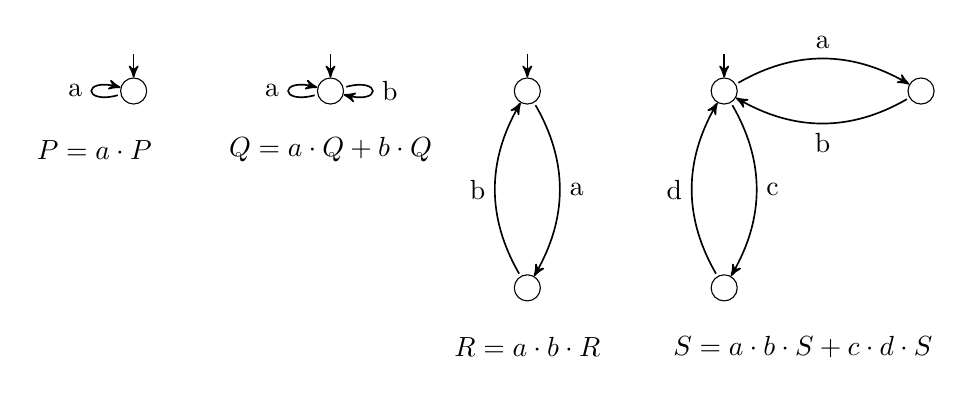
\begin{tikzpicture}
  \tikzstyle{state}=[draw,circle,node distance=25mm]
  \tikzstyle{arrow}=[->,shorten <=1pt,>=stealth',semithick]
  % P = a . P
  \node (n0) [state] {};
  \draw (n0) + (-0.5, -0.75) node {$P = a \cdot P$};
  \draw [arrow] (n0) + (0,0.5) to (n0);
  \draw [arrow,loop left] (n0) to node [auto] {a} (n0);
  % Q = a . Q + b .Q 
  \node (n1) [state,right of=n0] {};
  \draw (n1) + (0, -0.75) node {$Q = a \cdot Q + b \cdot Q$};
  \draw [arrow] (n1) + (0,0.5) to (n1);
  \draw [arrow,loop left] (n1) to node [auto] {a} (n1);
  \draw [arrow,loop right] (n1) to node [auto] {b} (n1);
  % R = a . b . R
  \node (n5) [state,right of=n1] {};
  \node (n6) [state,below of=n5] {};
  \draw (n6) + (0, -0.75) node {$R = a \cdot b \cdot R$};
  \draw [arrow] (n5) + (0,0.5) to (n5);
  \draw [arrow, bend left] (n5) to node [auto] {a} (n6);
  \draw [arrow, bend left] (n6) to node [auto] {b} (n5);
  % S = a . b . S +  c . d . S
  \node (n2) [state,right of=n5] {};
  \node (n3) [state,right of=n2] {};
  \node (n4) [state,below of=n2] {};
  \draw (n4) + (1.0, -0.75) node {$S = a \cdot b \cdot S + c \cdot d \cdot S$};
  \draw [arrow] (n2) + (0,0.5) to (n2);
  \draw [arrow, bend left] (n2) to node [auto] {a} (n3);
  \draw [arrow, bend left] (n3) to node [auto] {b} (n2);
  \draw [arrow, bend left] (n2) to node [auto] {c} (n4);
  \draw [arrow, bend left] (n4) to node [auto] {d} (n2);
 \end{tikzpicture}
 \caption{\label{fig:lpsexample} Examples of several LTS-es}
\end{figure}

\section{The parallel operator}
\label{ref:parallelop}

In the first section, we have somewhat informally described the $\parallel$ operator as an operator which given two processes results in the behavior of these two processes in parallel. In order to illustrate the way this works, let us consider the expected behavior of process $P \parallel Q$. There are three possibilities:

\begin{itemize}
\item Process $P$ performs an action before process $Q$
\item Process $Q$ performs an action before process $P$
\item Both processes perform an action simultaneously.
\end{itemize}

Let us illustrate this by considering a small example, consisting of process $P = a \cdot b$, process $Q = c$ and process $Z = P \parallel Q$. While we can formally derive process $Z$ (this is performed in Appendix \ref{apx:proofs}), it is also possible to do so by simply following the three possibilities outlined above. We shall use these to construct process $Z  = P \parallel Q$. First of all, note that the very first possibility is that process $P$ performs an action, which results in an $a$ action. Likewise, it's also possible that process $Q$ performs an action, which is action $c$. Finally, both processes can perform an action simultaneously, which would result in the multi-action $a \comm c$. The result is illustrated in Figure \ref{fig:par1} - we have numbered all states so we can refer to them.

\begin{lts}{fig:par1}{Under-construction LTS of process $Z = (a \cdot b) \parallel c$, step 1}
 \node (n0) [state] {0};
 \draw [arrow] (n0) + (0,0.5) to (n0);
 \node (n1) [state,below left of=n0] {1};
 \node (n2) [state,below of=n0] {2};
 \node (n3) [state,below right of=n0] {3};
 \draw [arrow] (n0) to node [auto] {$a$} (n1);
 \draw [arrow] (n0) to node [auto] {$a \comm c$} (n2);
 \draw [arrow] (n0) to node [auto] {$c$} (n3);
\end{lts}

Now, the next action can be performed. Let us consider the case in which process $P$ has performed an $a$ action. The only options are for process $P$ to perform an action, which must be action $b$ (since the $a$ has already occurred). Process $Q$ can also perform an action, which is action $c$. Finally, the $b$ and $c$ actions can be performed simultaneously, resulting in $b \comm c$. The result is illustrated in Figure \ref{fig:par2}.

\begin{lts}{fig:par2}{Under-construction LTS of process $Z = (a \cdot b) \parallel c$, step 2}
 \node (n0) [state] {0};
 \draw [arrow] (n0) + (0,0.5) to (n0);
 \node (n1) [state,below left of=n0] {1};
 \node (n2) [state,below of=n0] {2};
 \node (n3) [state,below right of=n0] {3};
 \node (n4) [state,below left of=n1] {4};
 \node (n5) [state,below of=n1] {5};
 \draw [arrow] (n0) to node [auto] {$a$} (n1);
 \draw [arrow] (n0) to node [auto] {$a \comm c$} (n2);
 \draw [arrow] (n0) to node [auto] {$c$} (n3);
 \draw [arrow] (n1) to node [auto] {$b$} (n4);
 \draw [arrow] (n1) to node [auto] {$c$} (n2);
 \draw [arrow] (n1) to node [auto] {$b \comm c$} (n5);
\end{lts}

There is an interesting observation to be made: in Figure \ref{fig:par2}, why does doing an $c$ action in state $1$ result in ending up in state $2$ and not a new state? This question can also be rephrased: do we end up in different states if we perform an $a$ action followed by a $c$ action compared to when we perform an $a \comm c$ action, e.g. we perform an $a$ and $c$ action simultaneously. This is not the case: after we have performed an $a$ action in process $P$ followed by a $c$ action in process $Q$, process $P$ can only do a $b$ action while process $c$ cannot do anything anymore; the same holds if we do a $a \comm c$ action. We continue by considering the next action after which process $Q$ has performed a $c$ action. Process $Q$ cannot do anything anymore, so process $P$ has to do an $a$ action, as illustrated in Figure \ref{fig:par3}.

\begin{lts}{fig:par3}{Under-construction LTS of process $Z = (a \cdot b) \parallel c$, step 3}
 \node (n0) [state] {0};
 \draw [arrow] (n0) + (0,0.5) to (n0);
 \node (n1) [state,below left of=n0] {1};
 \node (n2) [state,below of=n0] {2};
 \node (n3) [state,below right of=n0] {3};
 \node (n4) [state,below left of=n1] {4};
 \node (n5) [state,below of=n1] {5};
 \draw [arrow] (n0) to node [auto] {$a$} (n1);
 \draw [arrow] (n0) to node [auto] {$a \comm c$} (n2);
 \draw [arrow] (n0) to node [auto] {$c$} (n3);
 \draw [arrow] (n1) to node [auto] {$b$} (n4);
 \draw [arrow] (n1) to node [auto] {$c$} (n2);
 \draw [arrow] (n1) to node [auto] {$b \comm c$} (n5);
 \draw [arrow] (n3) to node [auto] {$a$} (n2);
\end{lts}

We see that the reasoning above still holds in Figure \ref{fig:par3}: there is no difference between first doing an $a$ action followed by a $c$ action,  first doing a $c$ action followed by an $a$ action or doing an $a$ and $c$ action simultaneously - regardless of the order we take them in, we end up in state 2. This diamond-like shape is actually very common when visualizing statespaces, and it is known as the notion of \emph{confluence}: often, the order of two actions is not important as the resulting state is the same. This can lead to optimizations of the state space, as the whole state space doesn't need to be calculated in order to obtain this result. Finally, if we consider the remaining action that are still possible, we obtain:

\begin{lts}{fig:par4}{Completed LTS of process $Z = (a \cdot b) \parallel c$}
 \node (n0) [state] {0};
 \draw [arrow] (n0) + (0,0.5) to (n0);
 \node (n1) [state,below left of=n0] {1};
 \node (n2) [state,below of=n0] {2};
 \node (n3) [state,below right of=n0] {3};
 \node (n4) [state,below left of=n1] {4};
 \node (n5) [state,below of=n1] {5};
 \draw [arrow] (n0) to node [auto] {$a$} (n1);
 \draw [arrow] (n0) to node [auto] {$a \comm c$} (n2);
 \draw [arrow] (n0) to node [auto] {$c$} (n3);
 \draw [arrow] (n1) to node [auto] {$b$} (n4);
 \draw [arrow] (n1) to node [auto] {$c$} (n2);
 \draw [arrow] (n1) to node [auto] {$b \comm c$} (n5);
 \draw [arrow] (n3) to node [auto] {$a$} (n2);
 \draw [arrow] (n2) to node [auto] {$b$} (n5);
 \draw [arrow] (n4) to node [auto] {$c$} (n5);
\end{lts}

As illustrated by Figure \ref{fig:par1} to \ref{fig:par4}, even the parallel composition of two very simple processes results in quite a number of states. Often, these can be reduced by using the $\tau_I$ and $\encap{B}$ operators as illustrated in the previous sections. As derived in Lemma \ref{lemma:abcommc}, the resulting process of $(a \cdot b) \parallel c = a \cdot (b \cdot c + c \cdot b + b \comm c) + c \cdot a \cdot b + a \comm c \cdot b$, which is the same process as illustrated in Figure \ref{fig:par4}. The important notion here is that putting multiple processes in parallel results in a lot of previously unexpected possibilities, which is why formally modeling these processes is beneficial: conditions that are unexpected will always turn up sooner or later.

\section{An example}

In order to get a clearer view of this theory, let us consider the following example: suppose we have a very basic alarm clock, which starts sounding an alarm at 7:00 AM. Once it is sounding, the user has two options: the alarm can be switched off by pushing the off button or it can be postponed for 10 minutes by pushing the snooze button. This behavior is illustrated in the following algorithm:

\begin{myalgo}{AlarmClock}{}
 $alarmSounding \qlet false$ \label{ac:initas} \\
 \qwhile $forever$ \\
 \qdo \qif $alarmSounding$ \label{ac:alon} \\
      \qthen \qcomment{The alarm is sounding - handle buttons} \\
             \qif off button is pushed \label{ac:offbtn1} \\
             \qthen \qcomment{Alarm must be turned off} \\
                    Turn the alarm off \\
                    $alarmSounding \qlet false$ \label{ac:offbtn2} \\
             \qelse \qif snooze button is pushed \label{ac:snzbtn1} \\
                    \qthen \qcomment{We must delay the inevitable for 10 minutes} \\
                           Turn the alarm off \\
                           Wait for 10 minutes \\
                           Turn the alarm on  \label{ac:snzbtn2} \qfi \qfi \\
      \qelse \qcomment{The alarm is not sounding} \\
             \qif it is 7:00 AM \label{ac:wakey1} \\
             \qthen \qcomment{Wakey wakey!} \\
                    Turn the alarm on \\
                    $alarmSounding \qlet true$ \label{ac:wakey2}
\end{myalgo}

How have we constructed this algorithm? Generally, we have just followed our intuition and wrote down what we expect would work. Typically, the next task is to implement this system in some programming language and check whether it does what we intended. However, we will be using this algorithm to construct a process $P$ of the system. First of all, we need to define the actions that we will be using. Keep in mind that actions can represent either an incoming or outgoing event, as illustrated in Section \ref{sec:actions}.

\begin{tabularx}{\textwidth}{|l|X|}
\hline
\TT{AlarmOn}      & Start sounding the alarm \\
\hline
\TT{AlarmOff}     & Turn the alarm sound off \\
\hline
\TT{SnoozeButton} & The snooze button has been pushed \\
\hline
\TT{OffButton}    & The off button has been pushed \\
\hline
\TT{Timer}        & 7:00AM has arrived \\
\hline
\TT{Delay10}      & 10 minutes have passed \\
\hline
\end{tabularx}

There is only a single variable in the algorithm, $alarmSounding$. This variable is used to see if we need to react on any buttons pushed, so our process will need this variable as well. This means our process will be $P(alarmSounding: \mathds{B})$, and $alarmSounding$ is initially $false$ due to the assignment in line \ref{ac:initas}. Let us focus on lines \ref{ac:offbtn1} - \ref{ac:offbtn2}: if the alarm is sounding ($alarmSounding = true$), pushing the off button should stop the alarm sound. In our process, this would become:

\begin{displaymath} alarmSounding \rightarrow \TT{OffButton} \cdot \TT{AlarmOff} \cdot P(false) \end{displaymath}

What does this represent? If $alarmSounding$ holds (due to the conditional operator $\rightarrow$), attempt an \TT{OffButton} action. If this is successful, it will be followed by an \TT{AlarmOff} action and subsequently by process $P$ where the parameter (this is the $alarmSounding$ parameter) is $false$, as the alarm will no longer be sounding. This confirms with the algorithm lines \ref{ac:offbtn1} - \ref{ac:offbtn2}. Subsequently, we can list the behavior of the snooze button similarly:

\begin{displaymath} alarmSounding \rightarrow \TT{SnoozeButton} \cdot \TT{AlarmOff} \cdot \TT{Delay10} \cdot \TT{AlarmOn} \cdot P(alarmSounding) \end{displaymath}

Once again, we shall dissect this line piece by piece: if $alarmSounding$ holds, attempt a \TT{SnoozeButton} action. If this is successful, we will in sequence perform \TT{AlarmOff} - to switch the alarm sound off, a \TT{Delay10} action to wait for 10 minutes, \TT{AlarmOn} to start the alarm sound and finally, we return to our process without changing the parameter (since we just pass the same value of $alarmSounding$ to $P$ again). This corresponds with lines \ref{ac:snzbtn1} - \ref{ac:snzbtn2}. Finally, there is only the case left where the alarm needs to start sounding, which is:

\begin{displaymath} \lnot alarmSounding \rightarrow \TT{Timer} \cdot \TT{alarmOn} \cdot P(true) \end{displaymath}

If the alarm is not sounding, attempt a \TT{Timer} action. If this is successful, continue by turning the alarm on by means of an \TT{AlarmOn} action and continue our process while setting the $alarmSounding$ parameter to $true$. This confirms with the algorithm lines \ref{ac:wakey1} - \ref{ac:wakey2}. We list the complete specification of process $P$:

$P(alarmSounding:\mathds{B}) =$ \\
$~\hspace*{1cm} alarmSounding \rightarrow \TT{OffButton} \cdot \TT{AlarmOff} \cdot P(false)~+$ \\
$~\hspace*{1cm} alarmSounding \rightarrow \TT{SnoozeButton} \cdot \TT{AlarmOff} \cdot \TT{Delay10} \cdot \TT{AlarmOn} \cdot P(alarmSounding)~+$ \\
$~\hspace*{1cm} \lnot alarmSounding \rightarrow \TT{Timer} \cdot \TT{alarmOn} \cdot P(true)$ \\

Why do we claim this specification $P$ is correct? First of all, note that the \TT{OffButton}, \TT{SnoozeButton} and \TT{Timer} actions are always the first actions in a row to be performed in a conditional. This means, if the condition holds, we will attempt one of these actions. The intuition is that, suppose the user does not push the off button, the \TT{OffButton} action is blocked. This means the first line will become:

\begin{displaymath} alarmSounding \rightarrow \delta \cdot \TT{AlarmOff} \cdot P(false) \end{displaymath}

In Section \ref{sec:macomm}, we have seen that if we are able to chose between an action $a$ or $\delta$, we always chose action $a$ since we want to avoid the deadlock. However, suppose all these actions are unavailable, then we would have no choice but to do a deadlock. Yet, there is an important aspect we have not illustrated so far: a process does not \emph{have} to perform an action - this can be delayed. Usually, if only deadlock actions are available, we will attempt to wait until something will become available - which makes perfect sense since these actions are initiated by some event. More importantly, a deadlock will only show if all possible actions can never occur, which is usually what we wish to analyze.

Finally, we shall present an LTS of process $P$ in Figure \ref{fig:aclts}. We note that the behavior of the system is clearly visible in the LTS, especially compared to the algorithm.

\begin{lts}{fig:aclts}{LTS of process $P$, the alarm clock example}
 \node (n0) [state] {};
 \draw [arrow] (n0) + (-0.5,0) to (n0);
 \node (n1) [state,right of=n0] {};
 \node (n2) [state,right of=n1] {};
 \node (n3) [state,right of=n2] {};
 \node (n4) [state,right of=n3] {};
 \node (n5) [state,right of=n4] {};
 \node (n6) [state,above of=n1] {};
 \draw [arrow, bend right] (n0) to node [auto,swap] {\TT{Timer}} (n1);
 \draw [arrow, bend right] (n1) to node [auto,swap] {\TT{alarmOn}} (n2);
 \draw [arrow, bend right] (n2) to node [auto,swap] {\TT{snoozeButton}} (n3);
 \draw [arrow, bend right] (n3) to node [auto,swap] {\TT{alarmOff}} (n4);
 \draw [arrow, bend right] (n4) to node [auto,swap] {\TT{Delay10}} (n5);
 \draw [arrow, bend right] (n2) to node [auto,swap] {\TT{offButton}} (n6);
 \draw [arrow, bend right] (n6) to node [auto,swap] {\TT{alarmOff}} (n0);
 \draw [arrow, bend right] (n5) to node [auto,swap] {\TT{alarmOn}} (n2);
\end{lts}



\chapter{Operation}
\label{sec:operation}

% wat moeten nodes nu eigenlijk weten?
% wat is de manier van werken? misschien iets over fases
% hoe is dit te modelleren?
% nog wat roepen over dat dit gebaseerd is op wim's verhaal?

As outlined previously, all nodes are identical, their respective identification number being the only exception. How will a node know when it has to switch its light on or off and how are they kept synchronized? A standard way of dealing with such situations is to introduce the concept of a \emph{leader}. This leader is responsible for initiating actions which should eventually lead to the desired behavior of the system. Initially, the leader must determine the properties of the network in use and relay necessary information to all other nodes in the system: each node has to know who the leader is, the node's coordinates in the network and what the actual size of this network is. Once the environment is properly set up, the leader will instruct all nodes which figure they should display. As each node knows the size of the network, its coordinates within this network and who the leader is, they will know whether they should switch their light on or off depending on the requested figure. The need for each of these properties will be elaborated in the next sections.

%Why is the information above sufficient? Strictly speaking, a node only needs to know whether it should act as the leader. However, as the available information is so limited, knowing which node is the leader is mandatory in order to detect multiple leaders. For example, if a node with a lowest identification number than whatever is currently in the network has been added, it will not know the configuration of the network, whereas the previous leader will have this information available. Thus, it makes more sense to detect this situation and force reinitialization of the network than just to assume the network will restore itself in time, which is something that may never occur.

Since all nodes have pretty limited resources (these are discussed in Section \ref{sec:hardware}), we intend to store as little information as possible. To this end, if a node knows the size of the network and its coordinates within this network, it can determine whether the light should be switched on or off - this removes the need for the leader to calculate per node if the light should be on or off; it can simply request a figure from all nodes and the nodes determine by themselves if the light should be turned on or off depending on their coordinates in the network, the network size and the figure to be displayed.

Based on this rough description, we can enumerate the steps needed in this system:

\begin{enumerate}
\item Leader election \\
As all nodes are identical, they need to agree on who will be the leader. This leader is used to initiate any further communication.
\item Node coordinates \\
The leader's first task is to determine the size of the network. However, before this can be done, every node must be assigned \emph{coordinates}, which must be unique in the network. The leader considers itself to be at \coord{0,0}, the other nodes are positioned relative to these coordinates and assume the same rotation as the leader node (i.e. the receiving node alters the meaning of its directions, resulting in it considering direction $0$ to be the same direction as the leader node considers it to be)
\item Network size determination \\
If all nodes have unique coordinates, we can determine the actual size of the network in use by determining the minimal and maximal $x$- and $y$-coordinates. This is necessary since a node initially has no idea what the size of the network in use is. We relay the minimum and maximum $x$- and $y$-coordinates throughout the network allowing every node to calculate the size of the network. The combination of grid size along with the node's coordinates is enough to determine whether the light should be switched on or off for each figure.
\item Showtime \\
Every node knows what it has to do to display the intended figure - the only catch is that nodes do not know when they have to change the figure. Since each node may run slightly faster or slower than the specified clock speed, we can't just let every node delay and change the figure - sooner or later, nodes will get out of sync this way. This is prevented by having the leader instruct all nodes when the time has come to alter the image that is currently being displayed.
\end{enumerate}

\begin{figure}
  \centering
  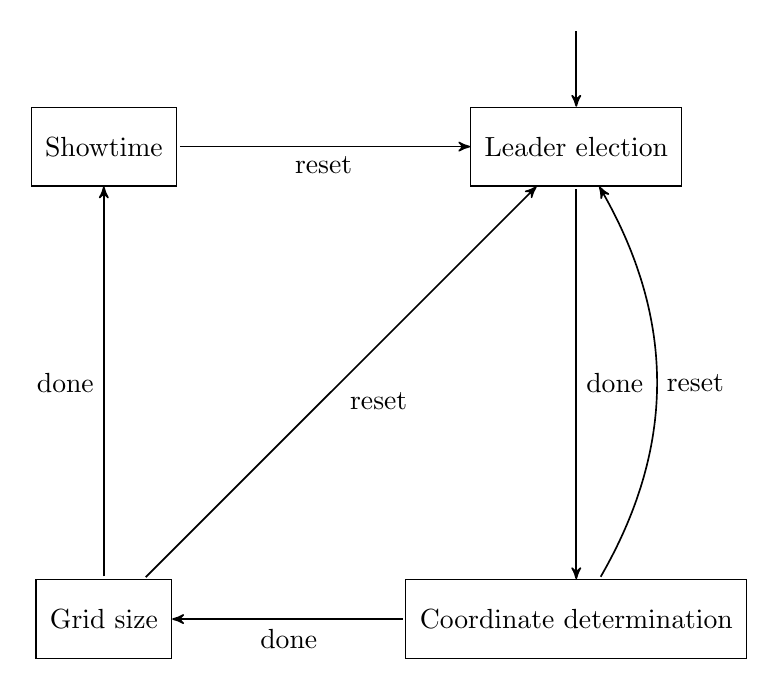
\begin{tikzpicture}
     \tikzstyle{state}=[draw,inner sep=5pt,minimum size=10mm,node distance=6cm]
     \tikzstyle{arrow}=[->,shorten <=1pt,>=stealth',semithick]
     \node (leader)   [state] {Leader election};
     \node (coord)    [state,below of=leader] {Coordinate determination};
     \node (gridsize) [state,left of=coord]   {Grid size};
     \node (showtime) [state,left of=leader]  {Showtime};
     \draw [arrow] (leader) + (0,1.5) to node [auto] {} (leader);
     \draw [arrow, right] (leader) to node [auto] {done} (coord);
     \draw [arrow] (coord) to node [auto] {done}  (gridsize);
     \draw [arrow] (gridsize) to node [auto] {done}  (showtime);
     \draw [arrow, bend right] (coord) to node [auto,swap] {reset} (leader);
     \draw [arrow, right] (gridsize) to node [auto,swap] {reset} (leader);
     \draw [arrow, right] (showtime) to node [auto,swap] {reset} (leader);
  \end{tikzpicture}
  \caption{\label{fig:statetrans} State transitions between the system steps}
\end{figure}

Observe that this outline does not consider externally altered node configurations. In fact, we have no way of detecting whether a node is added or removed at all. However, we can detect whether there are multiple leaders, since this may result in contradictory messages being received - one leader may request that all nodes display the first figure, whereas the other leader request the second figure; this may result in nodes constantly changing figures. Thus, if such a condition arises, the first node that observes there is an contradiction within the network must issue a \TT{reset} action to all neighboring nodes and resets itself, whereas nodes receiving this reset perform the same action (provided they have not already done so). The result is that a new leader is elected upon whom everyone agrees. To this end, we will also have to show that such a \TT{reset} action cannot occur under ordinary circumstances.

We shall graphically illustrate the flow between these steps in Figure \ref{fig:statetrans}. Each of these steps will be discussed in subsequent sections.


\section{Leader election}
\label{algo:leaderelection}

The very first operation is determining which node will become the leader. This is a well-known problem in distributed computing environments, for which many algorithms have been proposed. One of the first descriptions of such an algorithm can be found in \cite{lelann77distsys}, where leadership election in an unidirectional ring is discussed. Let us first illustrate such a ring in Figure \ref{fig:ringnetwork}. In an unidirectional ring, each node $i$ can only communicate with node $i+1$ and the final node $n$ can only communicate with node $1$; if the ring is bidirectional, node $i+1$ can also communicate with node $i$ and node $1$ can communicate with node $n$.

\begin{figure}
 \centering
 \begin{tikzpicture}
  \draw (0,0) circle (2cm);
  \foreach \angle/\n in {0/1, 60/n, 120/n-1, 180/..., 240/3, 300/2}
  {
   \filldraw (\angle:2cm) circle (1mm);
   \draw (\angle:2.3cm) node{$\n$};
  }
 \draw [->,xshift=0.5cm,semithick] (60:2cm) to [in=60,out=0] node  [auto] {unidirectional} (0:2cm);
 \draw [<->,xshift=-0.5cm,semithick,bend left] (190:2cm) to [in=180,out=0] node [auto,swap] {bidirectional} (240:2cm);
 \end{tikzpicture}
 \caption{\label{fig:ringnetwork} Structure of a ring network of $n$ nodes}
\end{figure}

In the algorithm described in \cite{lelann77distsys}, it is assumed that all nodes have a unique identifier with a total ordering. The result is a deterministic algorithm with a running time of $\OO(n^2)$ which can be improved to $\OO(n \log n)$ \cite{chang79decentextrma}. We note that construction of a deterministic algorithm is only possible if nodes have such a unique identifier \cite[Theorem 3.1]{lynch96distalgo}. If such a unique identifier is not present, it is possible to solve the problem using a randomized algorithm as discussed in \cite{itairodeh97symbreak}.

We will first discuss the relationship between our node networks, which we shall refer to a \emph{grid}, and the ring networks described in the literature. Note that unlike an ordinary grid, nodes in our grid network are only allowed to communicate with adjacent nodes.
\\
\begin{lemma} \label{lemma:grid2ring}
Let $G$ be a $n \times n$ grid. Then, there is no general way to transform $G$ to a ring containing $n*n$ edges.
\end{lemma} 
\begin{proof}
If we consider some $3 \times 3$ node configuration as $G$, we observe there is no way to transform $G$ to a $9$-edge ring: this is due to the fact that $G$ contains a node in the center, which prevents construction of such a ring as the grid only allows horizontal and vertical connections between nodes. This is illustrated in Figure \ref{fig:gridnode}, where the thick lines illustrate the two neighbors of each node. As can be seen, the node in the center cannot be connected without removal of some other node.

\begin{figure}[h]
\centering
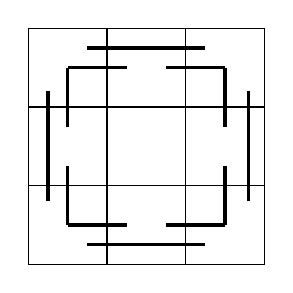
\begin{tikzpicture}
 \foreach \a/\b in { 0/0, 0/1, 0/2, 1/0, 1/1, 1/2, 2/0, 2/1, 2/2 } \draw (\a,\b) rectangle (\a+1,\b+1);
 \draw[very thick] ( 0.5, 0.50) -- (1.25, 0.50);
 \draw[very thick] ( 0.5, 0.50) -- ( 0.5, 1.25);
 \draw[very thick] (1.75, 0.50) -- (2.50, 0.50);
 \draw[very thick] (2.50, 0.50) -- (2.50, 1.25);
 \draw[very thick] ( 0.5, 1.75) -- ( 0.5, 2.50);
 \draw[very thick] ( 0.5, 2.50) -- (1.25, 2.50);
 \draw[very thick] (1.75, 2.50) -- (2.50, 2.50);
 \draw[very thick] (2.50, 2.50) -- (2.50, 1.75);

 \draw[very thick] (0.25, 0.80) -- (0.25, 2.20);
 \draw[very thick] (2.80, 0.80) -- (2.80, 2.20);

 \draw[very thick] (0.75, 2.75) -- (2.25, 2.75);
 \draw[very thick] (0.75, 0.25) -- (2.25, 0.25);
\end{tikzpicture}
\caption{\label{fig:gridnode} Attempt to transform $3 \times 3$ grid $G$ to a ring}
\end{figure}

Thus, since constructing a ring is already impossible for this specific grid $G$, it cannot be done in general as claimed.
\end{proof}

The previous lemma leads to an interesting observation: since a $3 \times 3$ grid $G$ cannot be transformed into a ring of $9$ edges, there cannot be a ring describing this specific $3 \times 3$ grid $G$. We obtain:
\\
\begin{corollary} \label{col:ring2grid}
Let $R$ be a ring containing $n * n$ edges. Then, there is no general way to transform $R$ to a grid of size $n \times n$.
\end{corollary}

From the two observations above, we conclude that we cannot use algorithms operating on ring networks. However, the study of ring networks is still useful to us: we can show that if leader election without unique identification numbers is not possible for ring networks, it cannot be done for grid networks either.
\\
\begin{theorem} \label{thm:needuid}
There is no deterministic algorithm $\mAA$ for leader election for any grid $G$ containing $n \times n$ edges if all nodes are completely identical.
\end{theorem}
\begin{proof}
Let us consider a grid $G$ of $2 \times 2$ nodes. Clearly, we can transform this grid to a ring as it is basically already a ring of $4$ edges. From \cite[Theorem 3.1]{lynch96distalgo} it follows that this problem cannot be solved without a way to distinguish the individual nodes, proving the theorem.
\end{proof}

Based on the hardware in use as outlined in Section \ref{sec:hardware}, we expect to have a pretty poor pseudo random generator. Based on this observation and Theorem \ref{thm:needuid}, it follows that the node identifiers are actually required. Fortunately, there is a unique identifier per node and we consequently use this identifier to elect a unique leader: the node with the lowest identifier becomes the leader. The following algorithm is proposed to carry out this procedure:

\begin{myalgo}{LeaderElection}{id}
 \qcomment{Initially, we believe we are the leader - but we haven't told anyone yet} \\
 $mustSend \qlet true$ \\
 $leaderid \qlet id$ \\
 \label{elect:loop} \qwhile leader election is in progress \\
 \label{elect:checksend} \qdo \qif $mustSend$ \\
  \qthen \qcomment{We haven't yet told who we believe the leader is} \\
         Send a message $(id, leaderid)$ to all directly connected nodes \\
         \label{elect:endsend} $mustSend \qlet false$ \qfi \\
  \label{elect:recv} \qif a message $(nodeid, newid)$ is received \\
  \qthen \qcomment{Someone believes he has new leader for us} \\
         \qif $newid < leaderid$ \\
         \qthen \qcomment{The proposed leader is better than the one we currently have} \\
                $leaderid \qlet newid$ \\
                \qcomment{Inform all our direct nodes about this new leader} \\
                \label{elect:recvdone} $mustSend \qlet true$ \\
         \qelse \label{elect:ign1} \qcomment{Our leader is better than what we received} \\
                \label{elect:ign2} \qignore \qfi \qfi \qelihw \\
  \label{elect:checkldr} \qcomment{We are done. If $id = leaderid$, we act as leader}
\end{myalgo}

First of all, line \ref{elect:loop} states that this algorithm should run while the leader election is in progress. This obviously begs the question: when is the leadership election done? The answer is that we cannot know - a leader does not keep an overview of all nodes, so it can't keep track of whether all nodes acknowledge their leader. And even if such a mechanism was to be implemented, if some node fails and never acknowledges the leader, we'd be waiting indefinitely. To prevent these issues, we say that the leader election phase ends if updates have not been received for 2 seconds. Even if the clock speed of all nodes may be off by a small percentage, the assumption is that messages are processed fast enough so that any lower identifier would have been received within this time.

By visual inspection of this rather straightforward algorithm, we expect it does the right thing: out of all nodes, the node with the lowest id becomes the leader. Since all id's are distinct, we know there is only one lowest id. Thus, a single node becomes the leader and all other nodes accept this course of action. However, can we provide a better founded argument? The algorithm will be described by means of a model in Chapter \ref{ch:leaderelection}, where it is proved that the necessary properties are satisfied.

\section{Coordinates determination}
\label{sec:opcoorddet}

Once a leader has been chosen, it must assign every node unique coordinates. The leader will consider itself to be at \coord{0,0} and in turn assign coordinates relative to this position to its neighboring nodes. However, nodes can be rotated any multiple of $90 \degree$, so it is important that all nodes in the network consider $0$ as the same direction, regardless of how each individual node is rotated. To this end, we must include the direction where the request should be received in the message, allowing the receiving node to determine how it is rotated and subsequently alter the meaning of its directions as needed. This results in all nodes assuming the rotation of the leader. Let us introduce how we can calculate the rotation based on the incoming and desired direction. Since all nodes are square-sized, they can be rotated $0 \degree, 90 \degree, 180 \degree$ and $270 \degree$. We shall introduce $r$ as a variable indicating the angle at which the node was rotated, where $rotation = r * 90 \degree$ to the right. The result is illustrated in Figure \ref{fig:rotations}.

\begin{figure}[h]
  \centering
  \begin{tikzpicture}
  \newcommand{\spnode}[6]{
   \draw (4*#1,0) rectangle (3+4*#1, 3);
   \draw (4*#1+1.5, 0.35) node {$#5$};
   \draw (4*#1+2.65,1.55) node {$#4$};
   \draw (4*#1+1.5, 2.65) node {$#3$};
   \draw (4*#1+0.35,1.55) node {$#6$};
   \draw (1.5+4*#1, -0.25) node {$r = #2$};
  }
   \foreach \a/\b/\c/\d/\e in { 0/0/1/2/3, 1/3/0/1/2, 2/2/3/0/1, 3/1/2/3/0 } \spnode{\a}{\a}{\b}{\c}{\d}{\e};
  \end{tikzpicture}
 \caption{\label{fig:rotations} Node rotation configurations, where $rotation = r * 90 \degree$}
\end{figure}

By looking at Figure \ref{fig:rotations}, we see that if an unrotated node ($r = 0$) is sending to direction $1$, a node with $r = 1$ would be sending to direction $0$, a node with $r = 2$ would be sending to direction $3$ and a node with $r = 3$ would be sending to direction $2$. There is a clear pattern here, which makes much more sense when we describe it: if some node $\mNN$ which is rotated $r$ turns to the right sends to direction $d$, this is the same as if an unrotated node would send to direction $d$ rotated $r$ turns to the left: the end result is the same.

By the above reasoning, we can define a rotate-left function, $rl(d,r) = (d - r) \mmod 4$: if the rotation is $r$ and the direction is $d$, the unrotated direction will be $d - r$, and since we have $4$ directions, we must perform the calculation modulo $4$. This function can also be used to find the actual rotation of a node: if we know the incoming direction $d$ and the expected direction $e$, we are interested in how much $d$ should be rotated to match $e$ - that is, we want to know what $e - d$ is, which is what $rl(e,d)$ calculates.

Once a node is aware of its rotation $r$, it can use this rotation to align its directions with the unrotated case. Let us consider an example: if a node has rotation $r = 2$ and it intends to send to unrotated direction $d = 1$, it should send to direction $3$, as illustrated in Figure \ref{fig:rotations}. As we have defined the rotation $r$ as the number of turns to the right, we can simply use output $(d + r) \mmod 4$ - this makes sense, as we are countering the left turns introduced by the $rl$ function. To this end, we appropriately introduce a rotate-right function $rr(d,r) = (d + r) \mmod 4$.

We need but one function: in order to determine the rotation of a node, we need the direction in which a message was received as well as the direction this message should have been received in. The first is available by means of the hardware (refer to Section \ref{sec:assumptions}), but the intended direction must be embedded in the message. Let us consider $r = 0$ in Figure \ref{fig:rotations}: if we send a message to direction $0$, we want it to be received in direction $2$. To this end, we can define a receiving-direction function $rd(i) = (i + 2) \mmod 4$.

Finally, we must define the coordinate system in use. To this end, we define the bottom-left coordinate as the lowest coordinate and subsequently, top-right is the highest coordinate in use. This is illustrated in Figure \ref{fig:relcoords}.

\begin{figure}[h]
\centering
\begin{nodefigure}
\nodegrid{3}{0}{0}{0/0/////, 1/0/\coord{ 0,-1}////, 2/0/////,
                   0/1/\coord{-1, 0}////, 1/1/\coord{0, 0}/$0$/$1$/$2$/$3$, 2/1/\coord{ 1, 0}////,
                   0/2/////, 1/2/\coord{ 0, 1}////, 2/2/////}
\end{nodefigure}
\caption{\label{fig:relcoords} Relative coordinates between nodes}
\end{figure}

Based on Figure \ref{fig:relcoords}, we can define a function $\Delta(c,d)$, which given a coordinate $c = \coord{x,y}$ and a direction $d$ returns the corresponding coordinate if coordinate $c$ is moved one position in direction $d$:

\begin{center}
\begin{tabular}{|l|l|}
\hline
\textbf{$d$} & \textbf{$\Delta(\coord{x,y}, d)$} \\
\hline
$0$     & $\coord{x,y+1}$ \\
\hline
$1$     & $\coord{x+1,y}$ \\
\hline
$2$     & $\coord{x,y-1}$ \\
\hline
$3$     & $\coord{x-1,y}$ \\
\hline
\end{tabular}
\end{center}

Using these definitions, we propose the following algorithm:

\begin{myalgo}{DetermineCoords}{id, actAsLeader}
 \qcomment{Initially, we always believe we are at \coord{0,0} and we are not rotated} \\
 $coord  \qlet \coord{0,0}$, $r \qlet 0$ \\
 \qcomment{The leader must initiate the procedure} \\
 $mustSend \qlet actAsLeader$ \\
 \qwhile coordinate determination is in progress \label{sp2:loop} \\
 \qdo \qcomment{Communicate new coordinates as necessary} \\
       \qif $mustSend$ \label{sp2:send1} \\
       \qthen \qcomment{Communicate coordinates to direction $i$} \\
              For all $0 \leq i \leq 3$: send coordinates $\Delta(coord, rr(i, r))$ using output $i$ \\
              where receiving direction should be $rr(rd(i), r)$ \\
              $mustSend \qlet false$ \qfi \label{sp2:send2} \\
      \qif a message $(newcoord, dir)$ has been received from direction $source$ \\
      \qthen \qif $coord = \coord{0, 0} \land \lnot actAsLeader$ \label{sp2:isinitial} \\
             \qthen \qcomment{We did not receive initial coordinates, so update them} \label{sp2:recinit1} \\
                    $coord \qlet newcoord$ \\
                    $r \qlet rl(dir, source)$  \\
                    \qcomment{We must inform our neighbors} \\
                    $mustSend \qlet true$ \qfi \label{sp2:recinit2} \\
             \qelse \qcomment{We already know our coordinates} \\ \label{sp2:recnext1}
                    \qif $coord \neq newcoord$ \\
                    \qthen \qcomment{We receive different coordinates - this indicates multiple leaders} \\
                           \label{sp2:rejectcoord} \qreset \\
                    \qelse \qcomment{Position is correct - check rotation} \\
                           \qif $rl(dir, source) \neq r$ \label{sp2:badrot} \\
                           \qthen \qcomment{Rotation is not correct} \\
                                  \qreset \\
                           \qelse \qcomment{We received the same coordinate on the correct input} \\
                                  \qignore \qfi \qfi \qfi \qfi \qelihw \label{sp2:recnext2}
\end{myalgo}

First of all, it must be noted that there are two approaches possible while sending updates in line \ref{sp2:send1} - \ref{sp2:send2}: we can either send to actual output pin $i$, regardless of its orientation or we can send to the pin that becomes output pin $i$ after countering the rotation. In our approach, we have chosen the first option as it makes the model clearer to understand and the second option doesn't provide any additional benefit.

The loop in line \ref{sp2:loop} has to terminate at some point - however, as before, we do not know when all nodes have been given coordinates as we do not know how many nodes there are. Thus, our only option is to continue to the next phase if we haven't received messages for a period of time, similar to leadership election.

Using the proposed algorithm, we note that once the rotation $r$ is calculated as $r = rl(d,n)$, we expect that sending a message back to $n$ using rotation $r$ by means of $rl(n,r)$ means we actually use direction $d$. This is proved in Lemma \ref{lemma:samedir}.
\\
\begin{lemma} \label{lemma:samedir} For any node number $n$ and direction $d$, it holds that $rr(n, rl(d,n)) = d$ \end{lemma}
\begin{proof}
\begin{derivation}{$rr(n, rl(d,n)) = d$}
\equ{Declaration $rr$}{$(n + rl(d,n)) \mmod 4 = d$}
\equ{Declaration $rl$}{$(n + ((d - n) \mmod 4)) \mmod 4 = d$}
\equ{Algebra}{$(n + d - n) \mmod 4 = d$}
\equ{Algebra}{$d \mmod 4 = d$}
\equ{$0 \leq d \leq 3$}{$true$}
\end{derivation}
\end{proof}

An interesting observation is that Lemma \ref{lemma:samedir} actually implies the condition in algorithm line \ref{sp2:badrot} cannot occur: if the leader sends a message from which the rotation is calculated, subsequent verification of the calculated rotation will always succeed. However, it is not specified whether nodes can be rotated without resetting them; if this behavior is possible, algorithm line \ref{sp2:badrot} can indeed occur and the result is that the system will reset itself as intended.

\section{Grid size determination}
\label{sec:opgridsize}

Once a node has entered this phase of the protocol, the node knows whether it is the leader, its coordinates within the grid and its rotation relative to the leader. However, the size of the grid is not known, while it is needed in order to determine which light should be switched on/off to display the intended figure. To this end, the grid size determination algorithm is run: each node communicates its maximal and minimal coordinates to its neighbors, which compare these coordinates to their current minimal and maximal coordinates. If this results in better (i.e. smaller minimum or greater maximum) coordinates, the node will update their current coordinates and communicate these to all adjacent nodes. The desired result is that every node learns the minimal and maximal coordinates in this grid, from which the total grid size can be derived.

First of all, we have to determine how coordinates are compared: when is one coordinate smaller or greater than another coordinate? In order to do this, keep in mind that we are looking for the bottom-left and top-right coordinates. In other words, coordinates $\coord{x_1, y_1} \leq \coord{x_2, y_2}$ if $x_1 \leq x_2$ and $y_1 \leq y_2$. The same goes for the maximum coordinates: $\coord{x_1, y_1} \geq \coord{x_2, y_2}$ if $x_1 \geq x_2$ and $y_1 \geq y_2$. This means the minimum of two coordinates are their smallest $x$ and $y$ values, whereas the maximum of two $x$ and $y$ values are their largest $x$ and $y$ values. Thus, $\mmin(\coord{x_1, y_1}, \coord{x_2, y_2}) = \coord{\mmin(x_1,x_2), \mmin(y_1,y_2)}$ and $\mmax(\coord{x_1, y_1}, \coord{x_2, y_2}) = \coord{\mmax(x_1,x_2), \mmax(y_1,y_2)}$.

Using these declarations, we propose the following algorithm to perform these actions:

\begin{myalgo}{DetermineGridSize}{id, actAsLeader, leaderid, coord}
 \qcomment{Initially, we believe our own coordinates are both the minimum and maximum} \\
 $minCoord, maxCoord \qlet coord, coord$ \\
 \qcomment{If we are leader, initiate the procedure. Otherwise, just wait} \\
 $mustSend \qlet actAsLeader$ \\
 \qwhile grid size determination is in progress \label{sp3:loopcond} \\
 \qdo \qcomment{Communicate new min/max coordinates as necessary} \\
       \qif $mustSend$ \label{sp3:sent1} \\
       \qthen \qcomment{Broadcast the min/max coordinates} \\
              Send $(leaderid, minCoord, maxCoord)$ to all outputs \\
              $mustSend \qlet false$ \qfi \label{sp3:sent2} \\
      \qif a message $(lid, minc, maxc)$ has been received \\
      \qthen \qcomment{Received a new message - check consistency} \\
             \qif $lid > leaderid$ \label{sp3:multil1} \\
             \qthen \qcomment{There are multiple leaders!} \\
                    \qreset \qfi \label{sp3:multil2} \\
             \qif $minc < minCoord$ \qor $maxc > maxCoord$ \\
             \qthen \qcomment{We have obtained smaller minimal or greater maximal coordinates} \label{sp3:new1}\\
                    $minCoord \qlet \mmin(minc,minCoord)$ \\
                    $maxCoord \qlet \mmax(maxc,maxCoord)$ \\
                    \qcomment{Update our leader id; $lid$ can only be less or equal to} \\
                    \qcomment{the current leader id} \\
                    $leaderid \qlet lid$ \\
                    \qcomment{Inform our neighbors about this} \\
                    $mustSend \qlet true$ \label{sp3:new2} \\
             \qelse \qcomment{We have a clearer picture of our grid than our neighbor. Yet, } \\
                    \qcomment{we may have received an even lower leader id so honor it} \\
                    $leaderid \qlet lid$ \qfi \label{sp3:ignore} \qelihw
\end{myalgo}

As usual, we should define what the condition in line \ref{sp3:loopcond} is: just looping forever waiting for new coordinates that never arrive can hardly be considered productive. However, like during the leader election, we cannot know if we have received the `correct' minimum/maximum coordinates, since each node cannot know what the network's minimum/maximum coordinate is - this is why we introduced this phase to begin with! Thus, all we can do is wait until we have not received updates for a certain period of time and assume the maximum coordinates has been received by then, similar to what we do in the leadership election phase.

\section{Showtime}

During this phase, all necessary information has been acquired: each node knows who the leader is, its coordinates within the grid and rotation relative to the leader and finally, the size of the grid in use. The only remaining part is that nodes should display the desired figures; these actions are initiated by the leader node. We assume that upon power-on, the light is switched off, since there is too little information available to start displaying a figure.

The following algorithm is proposed:

\begin{myalgo}{Showtime}{id, actAsLeader, leaderid,lpos,mincoord,maxcoord}
 \qwhile true \\
 \qdo \qcomment{The leader is responsible for initiating activity} \\
      \qif $actAsLeader$ \qand 2 seconds have elapsed \\
      \qthen \qcomment{The time has come} \\
	     $figure \qlet (figure +1 ) \mmod 2$ \label{sp4:timer1} \\
             Update light to confirm to $figure$ \\
             Send a message $(id,figure)$ to all directly connected nodes \label{sp4:timer2} \qfi \\
      \qif a message $(lid, newfigure)$ has been received \\
      \qthen \qif $lid > leaderid$ \\
             \qthen \qcomment{Someone else is pretending to be our leader} \\
                    \qreset \label{sp4:leadererr} \\
             \qelse \qif $figure \neq newfigure$ \\
                    \qthen \qcomment{Follow the leader} \\
                           $figure \qlet newfigure$ \label{sp4:sendfollow} \\
                           Update light to confirm to $newfigure$ \\
                           \qcomment{We may have received an even lower leader id, so honor it} \\
                           $leaderid \qlet lid$ \\
                           Send a message $(leaderid, newfigure)$ to all directly connected nodes \label{sp4:send2}\\
                    \qelse \qcomment{Our current status is fine, but the leader id may be lower} \\
                           $leaderid \qlet lid$ \label{sp4:ignupdate} \qfi \qfi \qelihw
\end{myalgo}

We note that we need a function which, given a node's coordinates, the minimal/maximal node coordinate and the figure that needs to be displayed determines whether the light should be switched on or off. We shall first give a specification for figures $0$ and $1$ as illustrated in Figure \ref{fig:showtimefig}.

\begin{figure}[h]
 \centering
 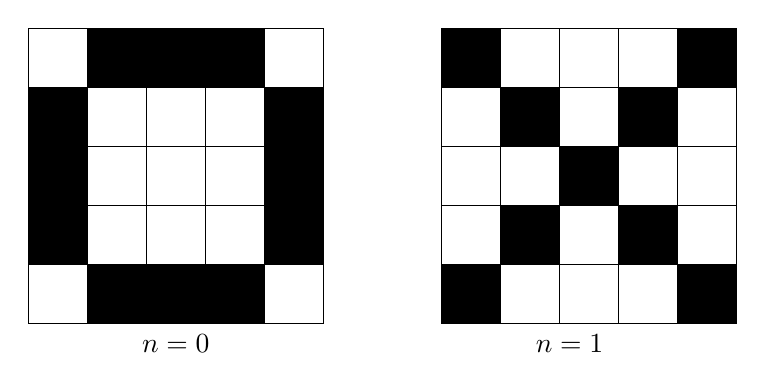
\begin{tikzpicture}
  \newcommand{\fillnode}[2]{\draw[fill] (0.75*#1,0.75*#2) rectangle (0.75+0.75*#1,0.75+0.75*#2);}
  \draw[step=0.75cm] (0, 0) grid (3.75,3.75);
  \foreach \a/\b in {
    1/0, 2/0, 3/0,
    0/1, 0/2, 0/3,
    4/1, 4/2, 4/3,
    1/4, 2/4, 3/4
  } \fillnode{\a}{\b};
  \renewcommand{\fillnode}[2]{\draw[fill] (5.245+0.75*#1,0.75*#2) rectangle (5.995+0.75*#1,0.75+0.75*#2);}
  \draw (1.875, -0.25) node {$n = 0$};
  \draw[step=0.75cm] (5.245, 0) grid (9,3.75);
  \foreach \a/\b in {
   0/0, 1/1, 2/2, 3/3, 4/4,
   0/4, 1/3,      3/1, 4/0
  } \fillnode{\a}{\b};
  \draw (6.875, -0.25) node {$n = 1$};
 \end{tikzpicture}
 \caption{\label{fig:showtimefig} Figures displayable by the nodes}
\end{figure}

The circular figure, $n = 0$, can be shown by lighting only the nodes at the border, with the exception of the nodes at the far edges. This gives the following formula:

\begin{tabbing}
\hspace{2cm} \= \\
$light(\coord{node_x,node_y}, \coord{min_x,min_y}, \coord{max_x,max_y}, \mbox{circle}) =$ \\
\> $(node_x = min_x \lor node_x = max_x \lor node_y = min_y \lor node_y = max_y)~\land$ \\
\> $\coord{node_x, node_y} \not\in \{ \coord{min_x, min_y}, \coord{max_x, min_y}, \coord{min_x, max_y}, \coord{max_x, max_y}$ \} \\
\end{tabbing}

As for the cross, determining the light state is a bit more involved. First of all, we want to normalize the grid coordinates, so that coordinate \coord{0,0} is the bottom-left. This is illustrated in Figure \ref{fig:coordnoorm}. Note that $min = \coord{-2, -1}$ and $max = \coord{0, 1}$ - to this end, we need to subtract $min$ from all coordinates.

\begin{figure}[h]
\centering
\begin{nodefigure}
\nodegrid{3}{0}{0}{0/0/\coord{-2,-1}////, 1/0/\coord{-1,-1}////, 2/0/\coord{ 0,-1}////,
                   0/1/\coord{-2, 0}////, 1/1/\coord{-1, 0}////, 2/1/\coord{ 0, 0}////,
                   0/2/\coord{-2, 1}////, 1/2/\coord{-1, 1}////, 2/2/\coord{ 0, 1}////}
\nodegrid{3}{4}{0}{0/0/\coord{ 0, 0}////, 1/0/\coord{ 1, 0}////, 2/0/\coord{ 2, 0}////,
                   0/1/\coord{ 0, 1}////, 1/1/\coord{ 1, 1}////, 2/1/\coord{ 2, 1}////,
                   0/2/\coord{ 0, 2}////, 1/2/\coord{ 1, 2}////, 2/2/\coord{ 2, 2}////}
\draw[->,>= stealth'] ( 5, 2.25) -- (5.5, 2.25);
\end{nodefigure}
\caption{\label{fig:coordnoorm} Coordinate normalization: bottom-left becomes \coord{0,0}}
\end{figure}

Now, we note that the bottom-left to top-right diagonal is simply determining whether the $x$ and $y$ coordinates are equal. The top-left to bottom-right coordinate means that the sum of the $x$ and $y$ coordinate is a fixed value: namely, the dimension of the grid minus 1. This gives the following formula:

\begin{tabbing}
\hspace{2cm} \= \\
$light(\coord{node_x,node_y}, \coord{min_x,min_y}, \coord{max_x,max_y}, \mbox{cross}) =$ \\
\> $x = y~\lor$ \\
\> $x + y = d$ \\
\textbf{where} \> $\coord{x,y} = \coord{node_x - min_x, node_y - min_y}$ \\
               \> $d = max_x - min_x$ \\
\end{tabbing}

\section{Resetting the system}
\label{sec:reset}

The previous algorithms all rely on a \TT{reset} action, which serves the purpose of instructing the complete node network to reset itself as something is flawed. Obviously, we need to describe this operation as we definitely do not intend to reset the system forever. To this end, upon power-on, a node must initialize $mustReset = false$ and $resetcount = 0$.

\begin{myalgo}{ResetAlgorithm}{}
\qwhile $true$ \\
  \qif $mustReset$ \\
  \qthen \qcomment{We haven't sent our reset to our neighbors yet} \\
         Send a message $resetcount$ to all directly connected nodes \\
         \qcomment{Increment the reset count, to ensure we do not honor this reset again} \\
         $resetcount \qlet (resetcount + 1) \mmod 10$ \\
         \label{reset:doit} Reset our current node \qfi \\
  \label{reset:recv} \qif a message $count$ is received \\
  \qthen \qcomment{We might have to reset} \\
         \qif $count \geq resetcount$ \\
         \qthen \qcomment{We must be resetting} \\
                $mustReset \qlet true$ \\
         \qelse \qcomment{We have already honored this reset round} \\
                \qignore \qfi \qfi \qelihw
\end{myalgo}

As can be seen, the $ResetAlgorithm$ algorithm runs forever - this is because the algorithm should always be active, as reset messages must be processed in any state of the system: $ResetAlgorithm$ must always run in parallel with the current algorithm in the system. Furthermore, the result of the \TT{reset} actions is that $mustReset$ should be set to $true$.

The actual reset performed in line \ref{reset:doit} should perform a reinitialization of the node. Specifically, the node should start in leader election phase, while $mustReset$ is set to $false$. The $resetcount$ value must not be changed, as this value is used to keep the network from resetting indefinitely.

\section{Research questions}
\label{sec:questions}

We will describe several research questions which will be answered in this thesis:

\begin{enumerate}
\item The system sketch describes distinct system modes and transitions between these modes. What is the system behavior if these modes are merged, i.e. any message can arrive in any mode? \\
This question is discussed in Sections \ref{sec:ignoreoop} to \ref{sec:ignorephase}.
\item Does the network adapt correctly if nodes are added or removed from the system? \\
This question is discussed in Section \ref{sec:alteringconfig}.
\item Can we determine how long a node should wait before electing itself as leader? \\
This question is discussed in Section \ref{sec:timedle}.
\item What happens if messages are not guaranteed to arrive? \\
This question is discussed in Section \ref{sec:unreliablecomm}.
\end{enumerate}

We will begin by proving correctness of the algorithms in a fixed configuration, under ideal circumstances: messages always arrive and the node configuration is never changed. The goal is to determine whether the algorithms we have presented are correct at all. In Chapter \ref{ch:overallsystem}, the influence of unreliable communication and adding/removing nodes will be discussed.

Chapters \ref{ch:leaderelection} to \ref{ch:showtime} all discuss the following $3 \times 3$ grid configuration:

\begin{figure}[h]
\centering
\begin{nodefigure}
\nodegrid{3}{0}{0}{0/2/0/$0$/$1$/$2$/$3$, 1/2/1/$1$/$2$/$3$/$0$, 2/2/2/$2$/$3$/$0$/$1$,
                   0/1/3/$3$/$0$/$1$/$2$, 1/1/4/$3$/$0$/$1$/$2$, 2/1/5/$0$/$1$/$2$/$3$,
                   0/0/6/$1$/$2$/$3$/$0$, 1/0/7/$0$/$1$/$2$/$3$, 2/0/8/$2$/$3$/$0$/$1$}
\end{nodefigure}
\caption{\label{fig:configused} The $3 \times 3$ node configuration used during the analysis in chapters \ref{ch:leaderelection} to \ref{ch:showtime}}
\end{figure}

Unfortunately, it is not possible to model an arbitrary configuration, as the statespace tends to grow so large in such situations that it is no longer manageable. Fortunately, a $3 \times 3$ grid seems sufficient to determine problems within the system; after completing the analysis of a $3 \times 3$ grid, an attempt has been made to analyze a $4 \times 4$ grid. The results were that even though the analysis took much longer, it did not yield any different results. This leads us to believe that analyzing a $3 \times 3$ grid is sufficient as it already illustrates any potential problems.

\chapter{General notes on the model}
\label{sec:generalnotes}

As outlined in the overview in Chapter \ref{sec:overview}, each node can only interact with four adjacent neighboring nodes. However, this has to be made explicit in our model: we need to define actions to interact between such nodes. This means we need some way to ensure whenever nodes interact, they can only do so with adjacent nodes and not just any node in the network. First of all, we define the size of the network as $\mDD \times \mDD$. In order to make this easier, we sequentially number the nodes, from $0 \dots N - 1$, where $N = \mDD^2$, the total number of nodes in the network. The idea is, that if we simply number nodes sequentially, we can determine whether nodes can communicate with each other based simply on their number. Note that we \emph{cannot} use node coordinates to determine whether this node can reach another node, since these coordinates are determined by an algorithm later on. Thus, the only purpose of the node number is to model the relationship between a node and its neighbors; it is different from the node's internal identification number. More on this distinction will be discussed later.

\begin{figure}[ht]
 \centering
 \begin{nodefigure}
  \nodegrid{3}{0}{0}{0/2/ 0////, 1/2/ 1////, 2/2/ 2////,
                     0/1/ 3////, 1/1/ 4/$0$/$1$/$2$/$3$, 2/1/ 5////,
                     0/0/ 6////, 1/0/ 7////, 2/0/ 8////}
 \end{nodefigure}
 \caption{\label{fig:gensetup} General setup of unrotated nodes in a $3 \times 3$ grid, thus $\mDD = 3$}
\end{figure}

Let us consider node number $4$ in the setup in Figure \ref{fig:gensetup}: this node can reach node number $1$ using direction $0$, node number $5$ using direction $1$, node number $7$ using direction $2$ and finally node number $3$ using direction $3$. We observe that the following relationship between node number $n$ and direction $d$ holds:

\begin{center}
\begin{tabular}{|l|l|l|}
\hline
\textbf{Direction} & \textbf{Node number} \\
\hline
$0$ & $n - \mDD$ \\
\hline
$1$ & $n + 1$ \\
\hline
$2$ & $n + \mDD$ \\
\hline
$3$ & $n - 1$ \\
\hline
\end{tabular}
\end{center}

However, just this relation is not enough: we have to explicitly disallow, for example node number $2$ communicating in direction $1$. By the above table, node number $2$ is able to communicate with node number $3$, which is not possible in reality. Therefore, we introduce extra constraints: nodes at the left edge of the grid cannot communicate in direction $3$, and likewise for nodes at the right edge in direction $1$, the top edge in direction $0$ and the bottom edge with $2$. Based on this specification, we define $neighbornum(n,d)$, which returns the node number of node number $n$'s neighbor in direction $d$ as:

\begin{displaymath}
neighbornum(n,d) = \left\{\begin{array}{rcl}
n - \mDD & \mbox{if} & d = 0 \land y > 0\\
n + 1   & \mbox{if} & d = 1 \land x < \mDD - 1\\
n + \mDD & \mbox{if} & d = 2 \land y < \mDD - 1\\
n - 1   & \mbox{if} & d = 3 \land x > 0\\
\end{array}\right.
\end{displaymath}
\begin{displaymath}
\begin{array}{rl}
\mbox{where} & x = n \mmod \mDD \\
             & y = n \mdiv \mDD \\
\end{array}
\end{displaymath}

Note that there are cases when we deliberately left $neighbornum$ unspecified: if such a condition arises, the node in question simply does not have a neighbor in the given direction.

Using this $neighbornum$ function, we can discuss how we send messages between nodes. Obviously, we cannot just tell messages to arrive - so we have to introduce actions for this purpose. To this end, each phase uses a $\TT{send(num,\dots)}$ action, which sends the specified parameters to a node number $num$ whereas an action $\TT{recv(num,\dots)}$ receives such a message. These actions are combined using communication action $\TT{comm(num,\dots)}$ - thus, if a process wishes to perform a \TT{send} action, there must be another process capable of doing a \TT{recv} action with identical parameters. However, this has an important consequence: since it is a communication action, every $\TT{send(num,\dots)}$ must have a corresponding $\TT{recv(num,\dots)}$ action in another process - which means we cannot simulate sending messages to nodes that do not exist, since such actions will be blocked. In reality, the hardware will just put signals on pins that are not connected to anything and since this does not change the internal state, this makes no difference.

If a message needs to be broadcast to all four adjacent nodes, it is safe to assume that this message is sent in a specific order: that is, the message will first be sent to direction $0$, then to direction $1$, etc. Thus, we introduce a process variable $s$ which contains the number of the direction we need to send to: if $s = 0$, we have to send to direction $0$, so once that has been accomplished, we increment $s$ as we now need to send to direction $1$. We repeat this for all directions, so if $s = 4$, this indicates we have sent to all directions. Should we subsequently need to send messages again, we can simply set $s = 0$.

Why do we need the distinction above? One may expect that just using four consecutive \TT{send} actions will have the same effect, and this is true if a node has four neighbors. If it does not, at least one of the \TT{send} actions will be blocked, as there is no corresponding \TT{recv} action. Clearly, this is not what we want, so we introduce an \TT{intern} action, which simulates putting a signal on a pin which will not be received. The result is that in our model, if a message needs to be sent to direction $s$, there are two possibilities: if there is indeed a neighbor at that direction, we use the \TT{send} action. If there is no neighbor, we use the \TT{intern} action to simulate that the node is sending a message but nobody receives it. Conveniently, we can re-use this notation in order to model the loss of messages, as we shall discuss later.

As stated in Section \ref{algo:leaderelection}, the node with the lowest unique identifier should become leader. To this end, we introduce a value $\mLL$, which is the number of the node that obtains identification number $0$ - and since all identification numbers are natural numbers, this is the lowest identification number and thus the leader node. We need to define a function to map a node's number to an unique identifier in such a way that the node which number equals $\mLL$ will obtain id $0$, whereas all other nodes will obtain unique id's that are greater than $0$; this is desirable as we want to be able to check the model for boundary conditions: we are not only interested in the case where the node with the lowest identification number is at the top-left of the network, but also what happens when we place it somewhere in the center of our network. To this end, we define a function $mapNodeId(num)$, which maps node number $num$ to a node $id$ in such a way that $mapNodeId(\mLL) = 0$ and all other numbers are distinct and greater than $0$. We use declaration $mapNodeId(num) = (num - \mLL) \mmod \mDD^2$, as it satisfies the specification above.

Since the required \TT{send}, \TT{recv} and \TT{comm} actions are different in each phase, we will not discuss their declarations here. However, the grid-positioning is always needed throughout the algorithms, so the corresponding mCRL2 declarations will be discussed now:

\begin{codeverb}
sort    Direction = Nat;
        Coord = struct coord(x:Int,y:Int);
\end{codeverb}

The first line declares the $Direction$ type, which is just a natural number, as it is in the previous discussions. The reason we declare it as a new type is to make it clearer in the models when we are dealing with a direction. The next line is the declaration of the $Coord$ type - a single $Coord$ is a combination of two integer values, the first being the $x$ coordinate and the latter being the $y$ coordinate.

\begin{codeverb}
map     DIM: Pos;
eqn     DIM = 3;

sort    RList = List(Nat);
map     RotationList: RList;
eqn     RotationList = [ 0, 3, 2, 1, 1, 0, 3, 0, 2 ];
\end{codeverb}

Since we always need the grid dimensions, we introduce a function $DIM$ which simply returns $\mDD$, the dimensions of the grid - in this case, a $3 \times 3$ grid. The same holds for the rotations: we use a list $RotationList$ containing $\mDD^2$ natural numbers. Each number denotes the number of right-rotations of the specified node. Thus, using the definition of $RotationList$ as above, node number $1$ would be rotated $3 * 90 \degree = 270 \degree$. The reasoning of using such a list is that once a node $n$ sends a message to direction $d$, we can use this list to transform direction $d$ based on the rotation of node $n$. If we introduced a parameter for each node indicating how much it is rotated, a node has information about its rotation. However, our goal is to introduction rotation as a malign force of nature: a node does not know whether it is rotated or how much, it just is, and it is up to the algorithms to decide how much this rotation actually is, as it is not possible for a node to circumvent the rotation.

In order to illustrate how this works, we first introduce the rotate-left and rotate-right functions $rl$ and $rr$ as discussed in Chapter \ref{sec:opcoorddet}:

\begin{codeverb}
map     rr: Direction#Int -> Nat;
var     d:Direction;
        n:Int;
eqn     rr(d,n) = (d+n) mod 4;

map     rl: Direction#Direction -> Nat;
var     d,e: Direction;
eqn     rl(d,e) = (d-e) mod 4;
\end{codeverb}

Then, using the $RotationList$ and the $rr$ function, we can introduce the concept of rotated nodes in our model: whenever node number $num$ intends to send to direction $d$, we should use output direction $rr(d,RotationList.num)$. So subsequently, the number of the node receiving the message is $neighbornum(num,rr(d,RotationList.num))$. This means the rotation of a node will always apply, and more importantly, this rotation is fixed.

\begin{codeverb}
map     neighbornum: Int#Direction->Int;
var     n:Int;
eqn     neighbornum(n,0) = if(n div DIM>0,n-DIM,n);
        neighbornum(n,1) = if(n mod DIM<DIM-1,n+1,n);
        neighbornum(n,2) = if(n div DIM<DIM-1,n+DIM,n);
        neighbornum(n,3) = if(n mod DIM>0,n-1,n);
\end{codeverb}

We define the $neighbornum$ function as illustrated previously, with one major difference. Previously, if there was no neighbor for node $n$ in direction $d$, we would leave $neighbornum(n,d)$ unspecified. However, in our models, we need to determine whether there is such a neighbor as we need to distinguish whether to use a \TT{send} or \TT{intern} action. Thus, we introduce an $if$ statement: if node $n$ has a neighbor in direction $d$, $neighbornum(n,d$) will return this neighbor. If there is no such neighbor, $neighbornum(n,d) = n$ .

\begin{codeverb}
map     move: Direction#Coord->Coord;
\end{codeverb}

We declare the $move$ function, which takes direction $d$ and coordinate $c$. The goal is to return coordinate $c$ moved one position in direction $d$, which is equivalent to $\Delta(c,d)$ as illustrated previously.

\begin{codeverb}
var     x,y: Int;
eqn     move(0,coord(x,y)) = coord(x,y+1);
        move(1,coord(x,y)) = coord(x+1,y);
        move(2,coord(x,y)) = coord(x,y-1);
        move(3,coord(x,y)) = coord(x-1,y);
\end{codeverb}

We introduce two dummy integer variables $x$ and $y$. For each direction, we specify the return value of the function, similar to how this is done in Figure \ref{fig:relcoords} and the corresponding table.

\begin{codeverb}
map     LEADERNUM: Pos;
eqn     LEADERNUM = 5;

map     mapNodeId : Nat -> Nat;
var     n:Nat;
eqn     mapNodeId(n) = (n - LEADERNUM) mod DIM*DIM;
\end{codeverb}

We have to specify which node will become the leader node. To this end, $LEADERNUM$ is equal to $\mLL$, the number of the node that should become leader. Finally, we define the $mapNodeId$ according to the definition given previously.

\chapter{Leadership election}
\label{ch:leaderelection}

Before we discuss any model, we have to consider a very important question: what exactly do we want to show? The goal of any model is to determine whether the system does `what it should do', so let us begin by defining what it should do: our goal is, to determine whether the leadership election algorithm as outlined in Section \ref{algo:leaderelection} always causes exactly one node to consider itself as a leader and whether all other nodes agree on the same leader. As outlined previously, we will only consider ideal circumstances throughout each individual algorithm model at first, as we want to determine whether the algorithms are correct at all. Analysis involving unreliable communication and modifying the network by adding or removing nodes will be covered in Chapter \ref{ch:overallsystem}.

As mCRL2 has difficulty analyzing timed models, we present two different models in this section: the first model is constructed in mCRL2 whereas the second model is constructed using UPPAAL.

\section{mCRL2 model}
\label{model:elect}

% wat is het algorithme in gebruik?
% basis idee achter hoe het model hiervan werkt
% bewijzen waarom het werkt

Naturally, we need a process for each SmartPixel - and since all SmartPixels have identical behavior, we just use the same process multiple times in parallel. We introduce actions \TT{sendID}, \TT{recvID} and \TT{commID} with parameters \emph{num,id} - these actions are used to respectively send, receive and communicate id \emph{id} to node number \emph{num}.

It seems we are on the right track now: each node can communicate what it believes to be the leader id to any adjacent node and this can be handled accordingly. However, one issue remains: the protocol specification states that after a few seconds, the leader election phase is done and thus a node that still considers itself to be the leader must become the leader. Unfortunately, the mCRL2 tools have difficulties analyzing models which involve timing. Thus, we try to prevent timing for now by coming up with some way to determine whether the desired result has been achieved; strictly speaking, we are checking whether the desired result \emph{will} occur, we are not considering \emph{when} it occurs. The latter can only be checked by analyzing the timed models, which we will attempt later on. By checking whether the desired result will occur we are actually proving correctness of the algorithm, which is desirable indeed.

Analyzing the algorithm reveals that at the end of the leader election phase, any node that has its own id as leader id will become a leader (line \ref{elect:checkldr}) - in other words, the node has not received an id which is lower than its own id. From this observation, it follows that if a node has ever received an id lower than its own id, it will \emph{never} become a leader. Thus, if we introduce a monitoring process that counts the number of nodes that receive a lower leader id while they still consider themselves as the leader, we are in business: if we have $n$ nodes in the network, the election phase ends if we have received word that $n-1$ nodes will not become leader.

To this end, we introduce the \TT{gotLeader} and \TT{monLeader} actions, all with parameters $num,id,initial$ which communicate together as \TT{commLeader}: these are used to indicate that node number $num$ received leader id $id$. The $initial$ boolean is $true$ if receiving $id$ results in the node demoting itself to an ordinary node: it will no longer become leader (We note that although it may seem we provide more information to the monitor than is necessary, this approach will allow us to check whether all nodes have the same leader later on by applying only minor changes to the leader process). The effect is that per node, $initial$ is $true$ at most one time: a node will initially consider itself leader and can only demote itself if it believed it was a leader. A process called \TT{LeaderMon} uses $monLeader$ actions to determine the number of nodes demoting themselves to ordinary nodes, by counting the number of $monLeader$ actions where $initial = true$. Once all but one node have declared they will not become leader, there is only a single node that tries to become leader. This is modeled using the \TT{tryLeader} and \TT{timeout} actions which communicate together as \TT{leader}: thus, a \TT{tryLeader} action can only be performed if there is a \TT{timeout} action available. This action is performed by \TT{LeaderMon} if all but one of the nodes have indicated they will not be a leader.

It must be noted that the above reasoning does not seem to confirm to the algorithm we are attempting to prove correct. Indeed, the algorithm as presented has absolutely no notion of how many nodes there are, let alone if they have a leader or not. Fortunately, this does not matter: we intend to show that always one node elects itself as leader. In our model, the final node only becomes a leader if all other nodes do not elect themselves as leader, which is essentially the same as waiting a fair period of time before concluding that since there apparently is no one else available, this node must be the leader.

Summarizing, we have the following actions:

\begin{itemize}
\item $\TT{gotLeader(num,leaderid,initial}) \comm \TT{monLeader(num,leaderid,initial)} \rightarrow \\ \TT{commLeader(num,leaderid,initial)}$ \\
The pair of \TT{gotLeader} and \TT{monLeader} actions are used to indicate that node number $num$ believes $leaderid$ to be the leader. $initial$ is true the first time the node has decided it will not become leader.
\item $\TT{sendID(num,id)} \comm \TT{recvID(num,id)} \rightarrow \TT{commID(num,id)}$ \\
These actions are used to send leader id $id$ to node number $num$.
\item $\TT{tryLeader(n)} \comm \TT{timeout(n)} \rightarrow \TT{leader(n)}$ \\
The \TT{tryLeader} action is issued by a node if it attempts to become leader; it is used in conjunction with \TT{timeout}, which is generated by the \TT{LeaderMon} process. The $n$ is the id of the node that tries to become leader.
\end{itemize}

We shall now illustrate the main \TT{Smartpixel1} process:

\begin{codeverb}
proc	Smartpixel1init(num:Nat) = @label{sp1:spinit}
	 Smartpixel1(num,mapNodeId(num),0); 

	Smartpixel1(num,leader_id,s:Nat) = @label{sp1:spproc}
\end{codeverb}

Line \ref{sp1:spinit} defines the \TT{Smartpixel1init} process - basically, this process becomes a \TT{Smartpixel1} process for a given node number $num$. The purpose of this process is to keep the initialization compact by providing defaults: each node considers itself as leader and has not yet sent any messages. Line \ref{sp1:spproc} defines the \TT{Smartpixel1} process. The parameters are the node number $num$ and the leader id $leader\_id$, plus a variable $s$ containing the next direction we need to send our leader id to.

\begin{codeverb}
(s<4&&(neighbornum(num,rr(s,RotationList.num))==num)) ->
    intern . Smartpixel1(num,leader_id,s+1) +
(s<4&&(neighbornum(num,rr(s,RotationList.num))!=num)) ->
    sendID(neighbornum(num,rr(s,RotationList.num)),leader_id) .
     Smartpixel1(num,leader_id,s+1) +
\end{codeverb}

If the leader id has not been communicated to a neighbor in direction $s$, we use the \TT{sendID} action as illustrated above to send the notification to the specified neighbor node. As \TT{commID} is a communication action, it is only permitted if there is a corresponding \TT{recvID} with the same arguments, so if there is no such neighbor we perform an \TT{intern} action. This corresponds to line \ref{elect:checksend} - \ref{elect:endsend} of the algorithm.

\begin{codeverb}
sum rid:Nat . (rid<leader_id) -> recvID(num,rid) .
                                  gotLeader(num,rid,mapNodeId(num)==leader_id) . @label{sp1:gotleader}
	                          Smartpixel1(num,rid,0) +
\end{codeverb}

As the algorithm dictates, if we receive any leader id $rid$ that is lower than what we currently consider as our leader ($rid < leader\_id$), we claim we have a leader by issuing the $gotLeader$ action where $initial = true$ if we considered ourself to be the leader ($mapNodeId(num) = leader\_id$) and $false$ otherwise. We finally update our process state by using $rid$ instead of $leader\_id$ as the leader id parameter, and $s = 0$ since we need to send this new leader id to our neighbors, like the algorithm requires (lines \ref{elect:recv} - \ref{elect:recvdone})

\begin{codeverb}
sum rid:Nat . (rid>=leader_id) -> recvID(num,rid) .
                                   Smartpixel1(num,leader_id,s) +
\end{codeverb}

If we receive the same leader or a leader that has a higher id than what we currently consider as the leader ($rid \geq leader\_id$), we do not update our internal state at all (lines \ref{elect:ign1} - \ref{elect:ign2}).

\begin{codeverb}
(mapNodeId(num)==leader_id) -> tryLeader(mapNodeId(num));
\end{codeverb}

If we believe we are the leader, we can perform a \TT{tryLeader} action; this is only possible if there is a subsequent \TT{timeout} action available since these communicate. This is outlined in line \ref{elect:checkldr} of the algorithm.

Where are the subsequent \TT{timeout} actions generated? These are performed by a monitoring process \TT{LeaderMon}. The idea is that this process collects the number of \TT{gotLeader} actions with $initial = true$, these are generated if a node decides it will not become a leader, which happens at most a single time per process, as previously argued. Since there are $n$ nodes in total, the \texttt{LeaderMon} process should wait for $n - 1$ \TT{gotLeader} actions before it may perform \TT{timeout} actions, which unblock \TT{tryLeader} actions and thus allowing nodes to assume the role of leadership. As \TT{gotLeader} and \TT{monLeader} communicate together, the \TT{LeaderMon} process should simply perform \TT{monLeader} actions:

\begin{codeverb}
LeaderMon(n:Int) =
 sum a,b:Nat . monLeader(a,b,true) . LeaderMon(n-1) +
 sum a,b:Nat . monLeader(a,b,false) . LeaderMon(n) +
\end{codeverb}

The first line simply defines the \TT{LeaderMon} process. The next two lines try to perform \TT{monLeader} actions, which are only possible if there is a corresponding \TT{gotLeader} action. If a node tells us it won't become leader (that is, the $initial$ parameter is $true$), we decrease the number of processes we are waiting for, since such an action will only happen a single time. If a \TT{gotLeader} action is performed by a process that already gave up its leadership role (the $initial$ parameter is $false$), we do not alter the number of processes and continue.

\begin{codeverb}
 sum a:Nat . (n<=0) -> timeout(a).LeaderMon(n);
\end{codeverb}

Finally, if we are no longer waiting for processes, we perform \TT{timeout} actions with parameter $a$ whenever possible, for any $a$ as we want to allow any remaining node id to become leader. These will cause the remaining processes that consider themselves as leader to be able to issue an \TT{tryLeader} action, which will become visible using the communication variant \TT{leader}.

It remains to specify the initializing process:

\begin{codeverb}
proc    System =
         allow({commID,leader,commLeader,timeout}, ( @label{sp1:allow}
          comm(sendID|recvID->commID,tryLeader|timeout->leader, @label{sp1:comm}
           gotLeader|monLeader->commLeader, ( 
            Smartpixel1init( 0) || Smartpixel1init( 1) || Smartpixel1init( 2) ||
            Smartpixel1init( 3) || Smartpixel1init( 4) || Smartpixel1init( 5) ||
            Smartpixel1init( 6) || Smartpixel1init( 7) || Smartpixel1init( 8) ||
            LeaderMon(DIM * DIM - 1)
           ))
          ));

init    System; @label{sp1:init}
\end{codeverb}

Line \ref{sp1:allow} specifies the actions we allow. We use this to block the explicit \TT{sendID}, \TT{recvID}, \TT{gotLeader}, \TT{monLeader}, \TT{tryLeader} and \TT{timeout} actions, as we are only interested in their communication variants. The next line specifies the communication between actions, which we have outlined previously. Finally, we list the processes: this is a $3 \times 3$ grid, totaling $9$ nodes. Thus, our monitor has to observe all but one node deciding they will not become leader before we unblock the \TT{leader} action.

\section{mCRL2 results}

As outlined previously, we want to show two different properties: only one leader gets elected, and all nodes agree on the same leader. We introduce two properties, which we prove by inspecting the mCRL2 models.
\\
\begin{property} \label{prop:oneleader}
The algorithm $LeaderElection$ as modeled in Section \ref{model:elect} always causes exactly one node to consider itself as the leader
\end{property}

\begin{proof}
We generate a labeled transition system of the model, where we hide everything except the $leader$ actions. Generating the state space using rooted branching bisimilarity (which is the equivalence relation we shall use from now on) of a $3 \times 3$ configuration yields Figure \ref{fig:elect1}.

\begin{statespace}{fig:elect1}{Leader election for Property \ref{prop:oneleader}, in which only the $leader$ action is visible}
 \initialstate{n0};
 \node (n1) [state,right of=n0] {1};
 \draw [arrow] (n0) to node [auto] {leader(0)} (n1);
\end{statespace}

We observe that there is only one path that always results in node $0$ becoming the leader, as claimed.
\end{proof}

Property \ref{prop:oneleader} can also be expressed using two modal formulas (we disregard the parameters of the $leader$ action here, as these are not important):

\begin{itemize}
\item $[{\it true}^{\star} \cdot {\it leader} \cdot {\it true}^{\star} \cdot {\it leader}] {\it false}$ \\
This expresses it cannot happen that two consecutive \TT{leader} actions occur.
\item $[ {\overline{\it leader}}^{\star} ] \langle {\it true}^{\star} \cdot {\it leader} \rangle {\it true}$ \\
If a \TT{leader} action has not yet occured, it will eventually occur.
\end{itemize}

As expected, checking these formulas in the original model without hiding any actions results in all of them holding. We need the second formula to show that the \TT{leader} action indeed occurs in the model - if this was not the case, the first formula would always be true.

This leads us to prove our second statement:
\\
\begin{property} \label{prop:sameleader}
The algorithm $LeaderElection$ as modeled in Section \ref{model:elect} results in all nodes eventually ending up in a state where they agree upon the same leader.
\end{property}

\begin{proof}
In our current model, a node will perform a \TT{gotLeader(id,rid,id==leader\_id)} action once it receives a lower leader id $rid$ (refer to line \ref{sp1:gotleader} of the algorithm) - this action is then used to unblock nodes from assuming leadership. However, we can also replace this action by \TT{gotLeader(id,rid,rid==0)}, which means the \TT{timeout} will be blocked until all non-leader nodes believe that node $0$ is their leader. The resulting state space is shown in Figure \ref{fig:elect2}.

\begin{statespace}{fig:elect2}{Leader election for Property \ref{prop:sameleader} in which only the $leader$ action is visible}
 \initialstate{n0};
 \node (n1) [state,right of=n0] {1};
 \draw [arrow] (n0) to node [auto] {leader(0)} (n1);
\end{statespace}

We observe that the \TT{leader} action will always be performed, which means all non-leader nodes consider node $0$ as their leader, which is what we claimed.
\end{proof}

If we were to use a modal formula, we need to check that $[ {\overline{\it leader}}^{\star} ] \langle {\it true}^{\star} \cdot {\it leader} \rangle {\it true}$ holds, which is indeed the case.

\section{UPPAAL model}

As mentioned previously, mCRL2's current toolkit is not capable of analyzing timed models. Thus, we introduce a model in the UPPAAL modeling toolset \cite{bengtsson95uppaal}. In UPPAAL, systems are described by networks of timed automata. We will not discuss the precise definition of a timed automaton here, but rather illustrate the overall idea: an automaton consists of a set of states (visualized by circles) and transitions between those states (visualized by arrows). The first state the system starts in is called the \emph{initial state}, which is visualized by a double circle.

States can have \emph{invariants} attached to them: these are conditions that must hold as long as the system resides in that state. Consequently, if the invariant condition no longer holds, a transition to another state must be taken. If a state contains a condition, it is placed within the circle below the horizontal line.

Transitions can have up to four different attributes, all of which are optional. There may be an \emph{update}, consisting of a $variable \leftarrow expression$ combination: once the transition has been taken, the contents of $variable$ is set to $expression$. There may also be a \emph{guard}, which is a predicate that must be true for this transition to be taken. For example, if the condition is $z < 5$, the transition may only be taken if the value of $z$ is smaller than $5$. Another possible attribute is a \emph{selection} value, which represents choice of a value out of some domain: for example, if we have $b: Bool$, this indicates variable $b$ can assume any value from the $Bool$ domain, so in this case, $b = true$ or $b = false$. This $b$ can subsequently be used in other attributes. Finally, there may be \emph{synchronization}, which indicates interaction between multiple processes. There are two flavors: $comm!$ and $comm?$ - the first one indicates a $comm$ communication is outgoing, whereas the latter indicates a $comm$ communication is incoming. For example, if one process has a transition which contains $comm!$ and all other attributes are satisfied, another process that has a transition that contains $comm?$ and also having all other attributes satisfied will allow both transitions to be taken; this makes it possible to model communication between multiple processes. Synchronizations can have parameters as well: if some process contains a transition with $comm[true][false]!$ and another process has selection $b, c : Bool$ and $comm[b][c]?$ could cause \emph{both} transitions, the sending process as well as the receiving process, to be taken where $b = true$ and $c = false$. If there is a $comm!$ communication without a $comm?$ communication in another process, the process issuing the $comm!$ is not allowed to perform the transition.

In Figure \ref{fig:upleader}, a SmartPixel performing leader election is illustrated, where all conditions are always in a fixed order: selection, guard, synchronization and update. For each SmartPixel, $id$ is both the unique id associated with the SmartPixel as well as the number in the grid, $lid$ is the id which the pixel considers to be the leader (initially, a node considers itself to be the leader due to the $lid \leftarrow id$ assignment) and $y$ and $z$ are clock variables: these are initially zero, and will increase as time passes. However, they can be reset back to zero; this makes it convenient to model time relative to some event. The $sendID[a][id]$ communication represents sending and receiving id $a$ to node number $id$. As in the mCRL2 case, we introduce $nn(id,s)$, for which it holds that $nn(id,s) = neighbornum(id,s)$. Finally, we have a type $NodeSet$, which contains all possible node id's; for example, in a $3 \times 3$ network, $NodeSet = \{ 0, \dots, 8 \}$. The complete model is illustrated in Figure \ref{fig:upleader}.

\begin{uppaal}{fig:upleader}{Leader election model in UPPAAL}
  \initialinvstate{init}{\nodepart{lower} \small $z < 1$};
  \node (start)  [invstate,node distance=7cm,right of=init] {Start \nodepart{lower} \small $z \leq 12$};
  \node (normal) [state,above left of=start,node distance=5cm] {Normal};
  \node (leader) [state,below left of=start,node distance=5cm] {Leader};
  \node (s1)     [invstate,right of=start] {\nodepart{lower} \small $y \leq 1$};
  % initial->start
  \draw [arrow,text=\upUPDATE] (init) to node (a1) [auto] {lid $\leftarrow$ id, z $\leftarrow$ 0, s $\leftarrow 0$} (start);
  % start->start: sendid[j]? with j < lid
  \draw [arrow,loop above,min distance=4cm,text=\upUPDATE] (start) to node (a2) [auto] {lid $\leftarrow$ j, s $\leftarrow$ 0} (start);
  \draw [text=\upSYNC] (a2) + (0, 0.5) node {sendID[j][id]?};
  \draw [text=\upGUARD] (a2) + (0, 1.0) node {j $<$ lid};
  \draw [text=\upSELECT] (a2) + (0, 1.5) node {j: NodeSet};
  % start->s1: sendid!
  \draw [arrow,min distance=4cm,text=\upSYNC] (start) to node (a3) [auto] {sendID[lid][nn(id,s)]!} (s1);
  \draw [text=\upUPDATE] (a3) + (0, -0.5) node {s $\leftarrow$ s+1, y $\leftarrow$ 0} (start);
  \draw [text=\upGUARD] (a3) + (0,  0.5) node {s $<$ 4 $\land$ nn(id,s) $\neq$ id};
  % start->s1: ignore
  \draw [arrow,min distance=4cm,bend right,text=\upGUARD] (start) to node (a5) [auto] {s $<$ 4 $\land$ nn(id,s) = id} (s1);
  \draw [text=\upUPDATE] (a5) + (0, -0.5) node {s $\leftarrow$ s+1, y $\leftarrow$ 0} (start);
  % s1->start
  \draw [arrow,text=\upUPDATE] (s1) to node [auto] {z $\leftarrow$ 0} (start);
  % start->start: sendid[j]? with j >= lid
  \draw [arrow,loop below,min distance=4cm,text=\upSELECT] (start) to node (a4) [auto] {j: NodeSet} (start);
  \draw [text=\upGUARD] (a4) + (0, -0.5) node {j $\geq$ lid};
  \draw [text=\upSYNC] (a4) + (0, -1.0) node {sendID[j][id]?};
  % start->normal
  \draw [arrow,text=\upGUARD] (start) to node [auto] {id $\neq$ lid $\land$ z$>$10 $\land$ s=4} (normal);
  % start->leader
  \draw [arrow,text=\upGUARD] (start) to node [auto,swap] {id=lid $\land$ z$>$10 $\land$ s=4} (leader);
\end{uppaal}

\section{UPPAAL results}

As previously outlined, UPPAAL allows us to formulate requirements as a series of temporal logic formula's; the logic used is a subset of computational tree logic \cite{huth04logic}. The major difference is that modal operators may not be nested: each formula must contain only a single modal operator with either a $\Diamond$ or a $\Box$, the remainder of the formula cannot have any modal operators. To this end, we have formulated the following formula's:

\begin{enumerate}
\item $A \Diamond \forall_{i:NodeSet} (Node(i).Leader \lor Node(i).Normal)$ \\
A state in which all nodes are in the $Leader$ or $Normal$ state is eventually reachable.
\item $A \Box \forall_{i:NodeSet} \forall_{j:NodeSet} (Node(i).Leader \land Node(j).Leader \Rightarrow i = j)$ \\
There is never more than a single node in the $Leader$ state.
\item $A \Diamond \exists_{i:NodeSet} Node(i).Leader$ \\
Eventually, there will be at least a single node in $Leader$ state.
\item $A \Diamond \forall_{i:NodeSet} Node(i).lid = 0$ \\
All nodes end up in a state where they consider node id $0$ to be their leader.
\end{enumerate}

We note that items 2 and 3 together imply that eventually, there has to be exactly one leader. Combined with Property \ref{prop:oneleader}, the system has to end in a state where all but one nodes are in the $Normal$ state and a single node is in the $Leader$ state. Finally, item 4 insists that all nodes agree on the same leader.

Asking UPPAAL to perform verification of these formulas yields the conclusion that all these properties are satisfied.

\chapter{Node coordinates determination}

\section{The model}
\label{model:coords}

The immediate goal of this phase is clear: we want to show, that the $DetermineCoords$ algorithm results in all nodes receiving correct coordinates. To fulfill this goal, we intend to have all nodes report the coordinates they obtain to a monitor, which in turn counts the number of correct coordinates received. However, in order to do this, we must first define what the correct coordinates are. Let us consider how coordinates are defined: basically, this is the position of the node relative to the leader - in other words, the leader itself always resides at coordinates \coord{0, 0}. Thus, as illustrated in Figure \ref{fig:relcoords}, if a node at direction $0$ exists, it should obtain coordinates \coord{0,1}. From this observation, it follows that the desired coordinates of some node number $n$ is simply the difference between node $n$'s position and the position of the leader (note that we do not consider rotations here - this is not necessary, since all nodes assume the rotation of the leader once they have received their coordinates). However, there is an important observation to be made: as outlined in Chapter \ref{sec:generalnotes}, in the model nodes are numbered sequentially from $0 \dots N - 1$, where node $0$ is the top-left node and node $N - 1$ is the bottom-right node. Yet, our coordinate system as described in Figure \ref{fig:gensetup} considers bottom-left as the smallest $(x,y)$-coordinates and top-right the largest. Due to this distinction between the model and our coordinate system, we have to invert the $y$-coordinate. To this end, we define a function $calcCoord(n) = \coord{n \mmod \mDD - \mLL \mmod \mDD, \mLL \mdiv \mDD - n \mdiv \mDD}$ which calculates the coordinates of node number $n$. In mCRL2, this becomes:

\begin{codeverb}
map     calcCoord : Int -> Coord;
var     num:Int;
eqn     calcCoord(num) =
                  coord(num mod DIM - LEADERNUM mod DIM,
                        LEADERNUM div DIM - num div DIM);
\end{codeverb}

The first two lines are simply administration for defining the function and a dummy argument. The remaining lines define the $calcCoord(num)$ function as stated before.

We need to introduce actions in order to send and receive messages, as well as a communication action to connect these. To this end, consider the situation where node $A$ sends a message to node $B$: we introduce the actions \TT{sendCoord}, \TT{recvCoord} and \TT{commCoord}, all with parameters $num,coord,wantdir,recvdir$, where $num$ is the number of the node $B$, the receiving node (this is outlined in Chapter \ref{sec:generalnotes}), $coord$ are the coordinates which the sending node $A$ transmitted, $wantdir$ is the direction in which node $B$ should receive the message, whereas direction $recvdir$ is the direction in which node $B$ actually received the message. We define $\TT{sendCoord} \comm \TT{recvCoord} \rightarrow \TT{commCoord}$ in order to model communication between the processes.

There is a crucial piece of information that our model requires: if we are to issue a $recvCoord$ action, we must limit the direction from which the message can be received, since there is only one possible direction in which such a message can be received. How we can determine this direction? The intuition is that the node that sends the message will already have assumed the rotation of the leader. This argument holds by induction: initially, the leader issues all coordinates so the argument trivially holds. As for the induction case, the node initiating the communication already has the correct orientation, or it would not be initiating communication.

In order to determine the receiving direction $d'$ of a message given that it should arrive on direction $d$ on node $num$ with rotation $r$, we observe this is the difference between the node's rotation $r$ and the rotation of the leader node. However, the rotation of the leader is always zero: this means that the receiving direction is always relative to no rotation, from which it follows that the direction $d'$ on which the message arrives is simply direction $d$ left-rotated $r$ times: the node is right-rotated $r$ times, so we need to left-rotate it $r$ times in order to counter this. This means that $d' = rl(d,RotationList.num)$.

While inspecting the algorithm, we notice that once coordinates are received, the node will consider itself to be at these coordinates. Subsequently, receiving any other coordinates will result in \TT{reset} actions, as this could only happen if there are multiple leaders in the system. Once all nodes except the leader have received coordinates, we are done. To this end, we introduce the \TT{success} action in our model, along with actions to report and acknowledge coordinates \TT{reportCoord}, \TT{ackCoord}, all with parameters $num,coord$, which communicate together as $\TT{reportCoord} \comm \TT{ackCoord} \rightarrow \TT{coordAction}$. Once a node receives its coordinates, it will initiate the \TT{reportCoord} action, where $num$ is the node number and $coord$ are the coordinates it considers itself at. As before, we use a \TT{ResultMon} process which acknowledges \TT{reportCoord} actions and keeps track of how many correct coordinates have been reported. Once all nodes have reported correct coordinates, a \TT{success} action will be initiated.

Summarizing, we have the following actions:

\begin{itemize}
\item $\TT{sendCoord(num,coord,wantdir,recvdir)} \comm \TT{recvCoord(num,coord,wantdir,recvdir)} \\
       \rightarrow \TT{commCoord(num,coord,wantdir,recvdir)}$ \\
These actions are used to subsequently send, receive and communicate coordinates to a neighboring node.
\item $\TT{reportCoord(num,coord)} \comm \TT{ackCoord(num,coord)} \rightarrow \TT{coordAction(num,coord)}$ \\
Once node number $num$ receives coordinates $coord$, it performs \TT{reportCoord} action with said parameters. The monitor process uses \TT{ackCoord} actions to verify these coordinates.
\item \TT{success} \\
If all nodes but one (the leader, as it always resides on fixed coordinates) have reported their coordinates, the result monitor process will initiate a \TT{success} action if all coordinates were correct.
\item \TT{reset} \\
If a node has already received coordinates, yet receives new coordinates which do not agree on the previous ones, a \TT{reset} action must be initiated.
\end{itemize}

We will now illustrate the \TT{Smartpixel2} process:

\begin{codeverb}
proc    Smartpixel2init(num:Nat) =
         Smartpixel2(num,num==LEADERNUM,if(num==LEADERNUM,0,4),coord(0,0),0);

        Smartpixel2(num:Nat,actAsLeader:Bool,s:Nat,log:Coord,r:Int) =
\end{codeverb}

We introduce the \TT{Smartpixel2init} process, which is convenient for initializing the main \TT{Smartpixel2} process using default parameters. The node assumes its initial coordinates are $\coord{0,0}$, but only the leader will initialize sending coordinates to neighboring nodes. Finally, the rotation is initially $0$, causing nodes to assume they have not been rotated.

\begin{codeverb}
(s<4&&neighbornum(num,rr(s,RotationList.num))==num) -> intern .
          Smartpixel2(num,actAsLeader,s+1,log,r) +
sum d':Direction.(s<4&&neighbornum(num,rr(s,RotationList.num))!=num) ->
         sendCoord(neighbornum(num,rr(s,RotationList.num)),move(rr(s,r),log),
          rr(rd(s),r),d') .
         Smartpixel2(num,actAsLeader,s+1,log,r) +
\end{codeverb}

As illustrated in Section \ref{sec:generalnotes}, we calculate the neighbor node number using the $neighbornum$ and $rr$ functions. We then proceed to calculate the coordinate to send and the direction we want it to arrive in. The reason we need a sum over the receiving direction, is that the sending node cannot know at which direction such a message arrives - thus, we try to send the message to any receiving direction possible. The corresponding $recvCoord$ function will then in turn only accept a single receiving direction. This corresponds to lines \ref{sp2:send1} - \ref{sp2:send2} of the algorithm.

\begin{codeverb}
sum c:Coord,d,d':Direction.(log==coord(0,0)&&!actAsLeader&&d'==rl(d,RotationList.num)) ->
       recvCoord(num,c,d,d') . reportCoord(num,rl(d,d'),c) .
       Smartpixel2(num,actAsLeader,0,c,rl(d,d')) +
\end{codeverb}

If coordinates are received while we still consider us at position \coord{0,0} and we do not act as leader, we honor these coordinates and report them accordingly to the monitor process. We set $s$ to $0$, since we should inform our neighbors of their coordinates relative to our own. This corresponds to lines \ref{sp2:recinit1} - \ref{sp2:recinit2} of the algorithm.

\begin{codeverb}
sum c:Coord,d,d':Direction.(c!=log&&(log!=coord(0,0)||actAsLeader)) ->
       recvCoord(num,c,d,d') . reset +
\end{codeverb}

Once a node receives new coordinates ($c \neq log$) while it already knows its coordinates ($log \neq \coord{0,0} \lor actAsLeader$), any different coordinates must be rejected using initiation of the \TT{reset} action (line \ref{sp2:rejectcoord} of the algorithm).

\begin{codeverb}
sum d,d':Direction . ((log!=coord(0,0)||actAsLeader)&&d'==rl(d,RotationList.num)&&
      r==rl(d,d')) ->
       recvCoord(num,log,d,d') . Smartpixel2(num,actAsLeader,s,log,r) +
\end{codeverb}

If a node receives identical coordinates and the rotation matches, the status is unchanged (line \ref{sp2:recnext2} of the algorithm).

\begin{codeverb}
sum d,d':Direction . ((log!=coord(0,0)||actAsLeader)&&d'==rl(d,RotationList.num)&&
      r!=rl(d,d')) ->
       recvCoord(num,log,d,d') . reset;
\end{codeverb}

If a node receives identical coordinates but the rotation does not agree with what the node previously determined, a \TT{reset} action must be initiated (line \ref{sp2:badrot} of the algorithm).

We still need to specify the \TT{ResultMon} process, which uses \TT{ackCoord} actions to monitor the result of \TT{reportCoord} actions:

\begin{codeverb}
proc    ResultMon(ok:Int) =
         sum num:Nat.ackCoord(num,RotationList.num,calcCoord(num)) . ResultMon(ok+1) + @label{sp2:okpos}
         sum num,r:Nat,c:Coord. (c!=calcCoord(num)||r!=RotationList.num) ->
          ackCoord(num,r,c) . ResultMon(ok) + @label{sp2:badpos}
\end{codeverb}

The first line defines the \TT{ResultMon} process. There is a single parameters: \TT{ok} indicates how many valid node coordinates have been received. This is illustrated in the next two lines of the model: only if the position for node number $num$ is identical to $calcCoord(num)$ and the rotation matches the item in the rotation list, we increase $ok$ by one. Otherwise, we acknowledge the coordinate but do not change our status.

\begin{codeverb}
(ok>=(DIM*DIM-1)) -> success; @label{sp2:success}
\end{codeverb}

Finally, if all nodes except the leader have reported their coordinates, we are done - this implies the \TT{success} action will only be initiated if all nodes have successfully received their coordinates, which is what we wanted to determine.

It remains to specify the initializing process:

\begin{codeverb}
proc    System =
	 allow({commCoord,coordAction,success,reset}, ( @label{sp2:allow}
	  comm({sendCoord|recvCoord->commCoord,reportCoord|ackCoord->coordAction}, (
	     Smartpixel2init( 0) || Smartpixel2init( 1) || Smartpixel2init( 2) ||
	     Smartpixel2init( 3) || Smartpixel2init( 4) || Smartpixel2init( 5) ||
	     Smartpixel2init( 6) || Smartpixel2init( 7) || Smartpixel2init( 8) ||
             ResultMon(0,0)
          ))
         ));

init    System;
\end{codeverb}

Line \ref{sp2:allow} specifies the actions we allow. We use this to block the explicit \TT{sendCoord}, \TT{recvCoord}, \TT{reportCoord} and \TT{ackCoord} actions, as we are only interested in their communication variants. The next line specifies the communication between actions, which we have outlined previously. Finally, we list the processes: this is a $3 \times 3$ grid, totaling 9 nodes. We initialize our monitor process, which hasn't received any reports yet, so the parameter is zero.

\section{The results}

First of all, what do we intend to show? The goal is, that whenever $DetermineCoords$ ends, the coordinates of node number $num$ confirm to the output of the function $calcCoord(num)$. This property can be proved by inspecting the mCRL2 model.
\\
\begin{property} \label{prop:correctcoords}
The algorithm $DetermineCoords$ as modeled in Section \ref{model:coords} results in all nodes assuming coordinates $calcCoord(num)$, where $num$ is the subsequent number of the node in question.
\end{property}

\begin{proof}
We note that line \ref{sp2:okpos} of our model registers the number of correct positions reported. Subsequently, line \ref{sp2:success} initiates a \TT{success} action once all correct positions have been acknowledged. To this end, we generate a labeled transition system in which we only show the \TT{success} and \TT{reset} actions. The result is illustrated in Figure \ref{fig:grid}.

\begin{statespace}{fig:grid}{Grid determination in which only the \TT{success} and \TT{reset} actions are visible}
 \initialstate{n0};
 \node (n1) [state,right of=n0] {1};
 \draw [arrow] (n0) to node [auto] {success} (n1);
\end{statespace}

We observe that the \TT{success} action will always occur, which proves the algorithm $DetermineCoords$ as modeled in Section \ref{model:coords} results in the correct coordinates being assigned, as claimed.
\end{proof}

Property \ref{prop:correctcoords} can also be expressed as a modal formula, which is $[{\overline{\it success}}^{\star} ] \langle {\it true}^{\star} \cdot {\it success} \rangle {\it true}$: as long as a $success$ has not been performed, it must eventually be possible to do so. As expected, this property holds in the model.

\chapter{Grid size determination}

\section{The model}
\label{model:gridsize}

In order to check whether the algorithm determines the correct grid size, we need to introduce two functions: $makeMinCoords$ and $makeMaxCoords$ which determine the corresponding minimum and maximum coordinates of a $\mDD \times \mDD$ grid with leader number $\mLL$. Let us consider Figure \ref{fig:sizegrid}: we observe the minimum position is the bottom-left coordinate, \coord{-2,-1}, whereas the maximum position is the top-right coordinate, \coord{0,1}. The question is: how can we determine the minimum and maximum positions if we only know the grid dimensions and the leader node number? If we study the figure in more detail, we observe that the minimum position consists of the amount of nodes to the bottom-left of the leader node: there are two nodes to the left of the leader node and one node below the leader node, so the minimum position is \coord{-2,-1}. Likewise, the maximum position consists of the number of nodes to the top-right of the leader node: there is one node above the leader node, and zero nodes to the right of the leader node, so the maximum position is \coord{0,1}.


\begin{figure}[ht]
 \centering
 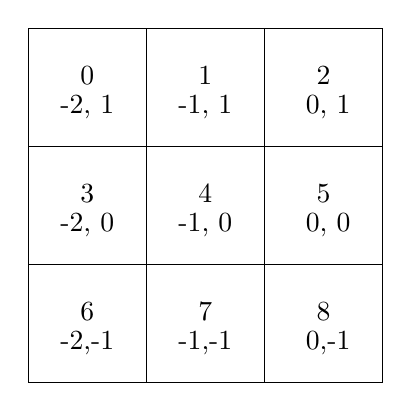
\begin{tikzpicture}
 % setnode{x}{y}{id}{pos}
 \newcommand{\setnode}[5]{
  \draw              (0.75+#1*1.5,0.90+#2*1.5) node {#3};
  \draw              (0.75+#1*1.5,0.50+#2*1.5) node {\coord{#4,#5}};
 }
 \draw[step=1.5cm] (3*1.5,3*1.5) grid (3*1.5+1.5*3,3*1.5+1.5*3);
 \foreach \a/\b/\c/\d/\e in { 0/2/0/-2/ 1,  1/2/1/-1/ 1,  2/2/2/ 0/ 1,
                              0/1/3/-2/ 0,  1/1/4/-1/ 0,  2/1/5/ 0/ 0,
                              0/0/6/-2/-1,  1/0/7/-1/-1,  2/0/8/ 0/-1 }
   \setnode{1.5*3+\a}{1.5*3+\b}{\c}{\d}{\e};
 \end{tikzpicture}
 \caption{\label{fig:sizegrid} Sample setup of a grid where $\mDD = 3$ and $\mLL = 5$}
\end{figure}

Since we know the dimensions of the grid and the nodes are numbered sequentially, we can easily determine the amount of nodes to the left of our leader: this is $\mLL \mmod \mDD$. The amount of nodes above our leader is $\mLL \mdiv \mDD$. Since grid $x$-coordinates are from left to right, the leftmost coordinate is the smallest, so the minimum $x$-coordinate is $-(\mLL \mmod \mDD)$. The grid $y$-coordinates are from bottom to top, which means that we need to determine the number of nodes above the leader node. This means the minimum $y$-coordinate is $-((\mDD-1) - (\mLL \mdiv \mDD))$.

Determining the maximum coordinates of the grid can be performed in a similar session: as stated, we need to determine the amount of nodes to the right of the leader node. Since there are $\mLL \mmod \mDD$ nodes to the left of the leader node, there are $(\mDD - 1) - (\mLL \mmod \mDD)$ nodes to the right of the leader node, so the maximum $x$-coordinate is $(\mDD - 1) - (\mLL \mmod \mDD)$. Finally, we need to determine the number of nodes above the leader node: this is $\mLL \mdiv \mDD$, which means the maximum $y$-coordinate is $\mLL \mdiv \mDD$. Summarizing, we can define $makeMinCoords = \coord{-a, -((\mDD - 1) - b)}$ and $makeMaxCoords = \coord{(\mDD - 1) - a, b}$ where $a = \mLL \mmod \mDD$ and $b = \mLL \mdiv \mDD$.

As usual, we need to introduce actions in order to model the communications. To this end, we introduce actions \TT{sendMinMax}, \TT{recvMinMax} and \TT{commMinMax}, all with parameters $num,leaderid,min,$ $max$: current leader id $leaderid$ and $min$, $max$ which are considered to be the minimum and maximum coordinates are communicated with node number $num$. Again, \TT{commMinMax} is the communication function between \TT{sendMinMax} and \TT{recvMinMax}.

Once a node retrieves updated min/max coordinates, we need some way to verify these. This is why we define the \TT{reportMinMax}, \TT{checkMinMax} and \TT{commMinMax2} actions, all using parameters $num,min,max$, stating node number $num$ has reported new minimum/maximum positions $min$/$max$. A monitor process uses \TT{checkMinMax} actions to validate the positions: whenever a node reports mix/max coordinates, we acknowledge them and keep track of the number of successful or invalid reports.

In order to be able to report that the desired state has been reached, we introduce \TT{success} and \TT{reset} actions as usual - the monitor process will issue a \TT{success} once all nodes have reported correct minimum/maximum coordinates.

Summarizing, we have the following actions:

\begin{itemize}
\item $\TT{sendMinMax(num,leaderid,min,max)} \comm \TT{recvMinMax(num,leaderid,min,max)} \\
       \rightarrow \TT{commMinMax(num,leaderid,min,max)}$ \\
These actions are used to send, receive and communicate leader id $leaderid$ and minimum/maximum coordinates $min$/$max$ to node number $num$.
\item $\TT{reportMinMax(num,min,max)} \comm \TT{checkMinMax(num,min,max)} \\
       \rightarrow \TT{commMinMax2(num,min,max)}$ \\
Once node number $num$ retrieves new min/max coordinates $min$/$max$, it will use a \\
\TT{reportMinMax} action to inform a monitor process, which uses the \TT{checkMinMax} action to verify the coordinates. 
\item \TT{success} \\
Once all nodes have reported their min/max coordinates, a \TT{success} action is issued if all coordinates are correct.
\item \TT{reset} \\
Whenever contradictory messages are being received, the node must be reset.
\end{itemize}

Before we discuss the main process, we need to declare functions that return the minimum and maximum of two coordinates, as outlined in Section \ref{sec:opgridsize}. We call these functions $minCoord$ and $maxCoord$ and give their corresponding declarations immediately:

\begin{codeverb}
map     maxCoord : Coord#Coord -> Coord;
        minCoord : Coord#Coord -> Coord;
var     x1,y1,x2,y2: Int;
eqn     maxCoord(coord(x1,y1),coord(x2,y2)) = coord(max(x1,x2),max(y1,y2));
        minCoord(coord(x1,y1),coord(x2,y2)) = coord(min(x1,x2),min(y1,y2));
\end{codeverb}

We will now introduce the model:

\begin{codeverb}
proc    Smartpixel3init(num:Nat) =
         Smartpixel3(num,num==LEADERNUM,mapNodeId(LEADERNUM),if(num==LEADERNUM,0,4),
                     calcCoord(num),calcCoord(num),calcCoord(num));

        Smartpixel3(num:Nat,actAsLeader:Bool,lid,s:Nat,log,mincoord,maxcoord:Coord) =
\end{codeverb}

We introduce the \TT{Smartpixel3init(num)} process, which is used for initialization of a leader or ordinary node based on the node number $num$. Initial default parameters are given to keep the initialization of the model more compact. We then introduce the \TT{Smartpixel3} process itself.

\begin{codeverb}
(s<4&&neighbornum(num,rr(s,RotationList.num))==num) -> intern .
    Smartpixel3(num,actAsLeader,lid,s+1,log,mincoord,maxcoord) +
(s<4&&neighbornum(num,rr(s,RotationList.num))!=num) ->
    sendMinMax(neighbornum(num,rr(s,RotationList.num)),lid,mincoord,maxcoord) .
    Smartpixel3(num,actAsLeader,lid,s+1,log,mincoord,maxcoord) +
\end{codeverb}

If a node has not sent its min/max coordinates to direction $s$, let it do so and the update $s$. This corresponds with lines \ref{sp3:sent1} - \ref{sp3:sent2} of the algorithm.

\begin{codeverb}
sum n:Nat,cmin,cmax:Coord . (n>lid) -> recvMinMax(num,n,cmin,cmax) . reset +
\end{codeverb}

If min/max coordinates are received from a higher leader id, it means there must be multiple leaders and we reset the system (lines \ref{sp3:multil1} - \ref{sp3:multil2}).

\begin{codeverb}
sum n:Nat,cmin,cmax:Coord . (n<=lid&&
    (minCoord(cmin,mincoord)!=mincoord||maxCoord(cmax,maxcoord)!=maxcoord)) ->
     recvMinMax(num,n,cmin,cmax) .
     reportMinMax(num,minCoord(cmin,mincoord),maxCoord(cmax,maxcoord)) .
     Smartpixel3(num,actAsLeader,n,0,log,
      minCoord(cmin,mincoord),maxCoord(cmax,maxcoord)) +
\end{codeverb}

If smaller minimum or greater maximum coordinates have been received, report them to the monitor process and update the process accordingly (algorithm lines \ref{sp3:new1} - \ref{sp3:new2})

\begin{codeverb}
sum n:Nat,cmin,cmax:Coord . (n<=lid&&minCoord(cmin,mincoord)==mincoord&&
    maxCoord(cmax,maxcoord)==maxcoord) ->
       recvMinMax(num,n,cmin,cmax) .
       Smartpixel3(num,actAsLeader,n,log,mincoord,maxcoord,s);
\end{codeverb}

If coordinates are received which do not influence the min/max coordinates we currently have, we only need to honor the leader id, which can only be smaller or equal than what we currently know (algorithm line \ref{sp3:ignore})

\begin{codeverb}
proc    ResultMon(ok:Int) =
         sum id:Pos,cmin,cmax:Coord . ((x(cmax)-x(cmin)+1 == DIM) &&
                                       (y(cmax)-y(cmin)+1 == DIM) &&
                                       ((cmin!=makeMinCoords)||(cmax!=makeMaxCoords))) ->
                                      checkMinMax(id,cmin,cmax) .  ResultMon(ok) +
\end{codeverb}

This is the \TT{ResultMon} process, with a single parameter $ok$. This parameter stores the number of correct min/max coordinates that have been received. The next line checks once the desired grid size of $\mDD \times \mDD$ is reported, whether the expected min/max coordinates have been received. If this is not the case, the status is not updated.

\begin{codeverb}
sum id:Pos,cmin,cmax:Coord . ((x(cmax)-x(cmin)+1 == DIM) &&
                              (y(cmax)-y(cmin)+1 == DIM) &&
                              (cmin==makeMinCoords&&cmax==makeMaxCoords)) ->
                             checkMinMax(id,cmin,cmax) .  ResultMon(ok+1) + @label{sp3:resultok}
\end{codeverb}

If a grid size is reported with min/max coordinates as expected and the dimensions are correct, we have one more node storing the correct min/max, so we update our state accordingly.

\begin{codeverb}
sum id:Pos,cmin,cmax:Coord . ((x(cmax)-x(cmin)+1 <  DIM) ||
                              (y(cmax)-y(cmin)+1 <  DIM)) -> 
                             checkMinMax(id,cmin,cmax) . ResultMon(ok) + @label{sp3:resultign}
sum id:Pos,cmin,cmax:Coord . ((x(cmax)-x(cmin)+1 >  DIM) ||
                              (y(cmax)-y(cmin)+1 >  DIM)) ->
                             checkMinMax(id,cmin,cmax) . ResultMon(ok) + @label{sp3:resultfail}
(ok>=DIM*DIM) -> success; @label{sp3:victory}
\end{codeverb}

Grid sizes that are smaller than the final dimensions can be ignored, as the nodes are probably still working out how large the grid is. However, it is obviously not correct if bigger dimensions are being reported than we actually expect, so do not register success in such a case. Finally, if all nodes have reported the grid size correctly, we initiate a \TT{success} action.

\begin{codeverb}
proc    System =
         allow({commMinMax,commMinMax2,success,reset}, (
          comm({sendMinMax|recvMinMax->commMinMax,reportMinMax|checkMinMax->commMinMax2}, (
             Smartpixel3init( 1) || Smartpixel3init( 2) || Smartpixel3init( 3) ||
             Smartpixel3init( 4) || Smartpixel3init( 5) || Smartpixel3init( 6) ||
             Smartpixel3init( 7) || Smartpixel3init( 8) || Smartpixel3init( 9) ||
             ResultMon(0)
          ))
         ));
\end{codeverb}

We begin by specifying the actions we allow. Again, this is used to block explicit \TT{sendMinMax}, \TT{recvMinMax}, \TT{reportMinMax} and \TT{checkMinMax} actions, since we are only interested in the communication between actions. Finally, we list the processes themselves.

\section{The results}

The goal of this phase is to determine whether all nodes receive the correct minimum and maximum grid coordinates, where the correct minimum coordinate is $makeMinCoords$ and the correct maximum coordinate is $makeMaxCoords$ as previously described.
\\
\begin{property} \label{prop:minmaxcoord} The algorithm $DetermineGridSize$ as modeled in Section \ref{model:gridsize} results in all nodes considering $makeMinCoords$ as minimum grid coordinates and $makeMaxCoords$ as maximum grid coordinates.
\end{property}

\begin{proof}
We note that line \ref{sp3:resultok} of the model increases the count of correct coordinates reported if the dimensions are correct and the coordinates reported are correct. Consecutively, line \ref{sp3:victory} reports success if and only if \emph{all} nodes have reported the correct position. Thus, we generate a labeled transition system in which we only show the \TT{success} and \TT{reset} actions. The result is illustrated in Figure \ref{fig:gridsvg}.

\begin{statespace}{fig:gridsvg}{Grid size determination in which only $success$ and $reset$ actions are visible}
 \initialstate{n0};
 \node (n1) [state,right of=n0] {1};
 \draw [arrow] (n0) to node [auto] {success} (n1);
\end{statespace}

We observe that the \TT{success} action will always be performed, whereas the \TT{reset} action will not. We observe that all nodes will end up in a state where they know the minimum/maximum grid coordinates as defined by $calcMinCoord$ and $calcMaxCoord$ as claimed.
\end{proof}

Property \ref{prop:minmaxcoord} can also be expressed as a modal formula, which is $[{\overline{\it success}}^{\star} ] \langle {\it true}^{\star} \cdot {\it success} \rangle {\it true}$: as long as a \TT{success} has not been performed, it must eventually be possible to do so. As expected, this property holds in the model.

\chapter{Showtime}
\label{ch:showtime}

\section{The model}
\label{model:showtime}

The desired goal of this phase is pretty obvious; the resulting system should only have two phases: one in which all lights are set up to display figure $0$ and one in which all lights are set up to display figure $1$. In the previous section, we have declared formulas that determine whether the light should be switched on or off, so we introduce an action \TT{updateLight} with parameters $n,f$ which indicates that node number $n$ updates its light to reflect the output of $light(pos_n, min_n, max_n, f)$, where $pos_n$ is the position of node $n$, $min_n$/$max_n$ are the minimum/maximum coordinates stored by node $n$ - whether this actually switches the light on or off doesn't need to be considered in the model.

We also need some way to communicate new status updates, so we introduce actions \TT{sendUpdate}, \TT{recvUpdate} and \TT{commUpdate}, all with parameters $num,leaderid,figure$, where $num$ is the node number to which the update is sent, $leaderid$ is the id that the sending node considers to be the leader and $figure$ is the new figure to be displayed. As usual, \TT{commUpdate} is a communication action between \TT{sendUpdate} and \TT{recvUpdate}.

The algorithm states that the leader should initiate the procedure by sending figure updates every two seconds. To this end, we introduction an action \TT{timer} that is issued when the two seconds have passed. Finally, the algorithm is also capable of resetting the system, so we introduce a \TT{reset} action.

Summarizing, we have the following actions:

\begin{itemize}
\item $\TT{sendUpdate(num,leaderid,figure)} \comm \TT{recvUpdate(num,leaderid,figure)}\\
       \rightarrow \TT{commUpdate(num,leaderid,figure)}$ \\
These actions are used to subsequently send, receive an communicate a figure update.
\item \TT{updateLight(n,f)} \\
This action is issued if node number $n$ updates its light to display figure $f$.
\item \TT{timer} \\
This action can be issued every two seconds, it is used to model the two-second timer.
\item \TT{reset} \\
If any node receives a message stating a leader that conflicts with its own leader, a \TT{reset} action is initiated.
\end{itemize}

We now introduce the model:

\begin{codeverb}
proc    Smartpixel4init(num:Nat) =
         updateLight(num,0) .
         Smartpixel4(num,num==LEADERNUM,mapNodeId(LEADERNUM),0,0,calcCoord(num));  @label{sp4:updstate1}

        Smartpixel4(num:Nat,actAsLeader:Bool,leaderid,figure,s:Nat,log:Coord) =
\end{codeverb}

We introduce the \TT{Smartpixel4init(num)} process, which used to initialize a node. This is used to pass predefined parameters to the \TT{Smartpixel4} processes in order to keep the initialization code readable. It remains to specify the main \TT{Smartpixel4} process:

\begin{codeverb}
(s<4&&neighbornum(num,rr(s,RotationList.num))==num) -> intern .
    Smartpixel4(num,actAsLeader,leaderid,figure,s+1,log) +
(s<4&&neighbornum(num,rr(s,RotationList.num))!=num) ->
    sendUpdate(neighbornum(num,rr(s,RotationList.num)),
     if(actAsLeader,mapNodeId(num),leader_id),figure) .
    Smartpixel4(num,actAsLeader,leaderid,figure,s+1,log) +
\end{codeverb}

If we need to send a status update in some direction, we do so - however, the leader must always use its own id while sending. This corresponds to lines \ref{sp4:timer2} and \ref{sp4:send2} of the algorithm.

\begin{codeverb}
sum n,a:Nat . (n > leaderid) -> recvUpdate(num,n,a) . reset +
\end{codeverb}

If a status update is received with a leader id that is higher than what we currently have, we initiate a \TT{reset} action, as is performed by line \ref{sp4:leadererr} of the algorithm.

\begin{codeverb}
sum n,a:Nat . (n <= leaderid && a != figure) -> recvUpdate(num,n,a) .
        updateLight(num,a) .
        Smartpixel4(num,actAsLeader,n,a,0,log) + @label{sp4:updstate2}
\end{codeverb}

If we receive an update with the correct leader id, we update our light status and reset all sender directions, which means we will transmit the new status to our neighboring nodes (algorithm lines \ref{sp4:sendfollow} - \ref{sp4:send2})

\begin{codeverb}
sum n:Nat . (n <= leaderid) -> recvUpdate(num,n,figure) .
        Smartpixel4(num,actAsLeader,n,figure,log,s) +
\end{codeverb}

If we receive the current figure we are displaying with an equal or lower leader id, update our leader id and continue (algorithm line \ref{sp4:ignupdate})

\begin{codeverb}
(actAsLeader) -> timer .       @label{sp4:timer}
           updateLight(num,(figure+1) mod 2) .
           Smartpixel4(num,actAsLeader,leaderid,(figure+1) mod 2,0,log);
\end{codeverb}

If we act as leader, we must initiate new state changes. This is done by updating our own initial light and figure and setting $s = 0$, so we will communicate this with our neighbors (algorithm lines \ref{sp4:timer1} - \ref{sp4:timer2}).

\begin{codeverb}
proc    System =
         allow({commUpdate,reset,updateLight,timer}, (
          comm({sendUpdate|recvUpdate->commUpdate}, (
             Smartpixel4init( 0) || Smartpixel4init( 1) || Smartpixel4init( 2) ||
             Smartpixel4init( 3) || Smartpixel4init( 4) || Smartpixel4init( 5) ||
             Smartpixel4init( 6) || Smartpixel4init( 7) || Smartpixel4init( 8)
          ))
         ));

init    System;
\end{codeverb}

We start by specifying the allowed actions; this implies we block explicit \TT{recvUpdate} and \TT{sendUpdate} actions. We continue by specifying the communication actions as before and finally, we list the Smartpixel processes.

\section{The results}

The idea of the showtime phase is that all nodes end up in a state where all nodes display figure $0$, followed by a timeout, followed by all nodes displaying figure $1$, etc. 
\\
\begin{property} \label{prop:showtime}
The algorithm $Showtime$ as modeled in Section \ref{model:showtime} results in all nodes alternating between a state in which they display figure $0$ and a state in which they display figure $1$; transitions between these states are made using \TT{timer} actions.
\end{property}

\begin{proof}
First of all, we note that by line \ref{sp4:timer}, a \TT{timer} action will cause the figure to be updated and this update communicated with neighboring nodes. Thus, what we want to show is that the system will keep performing \TT{timer} actions: it cannot happen that this action is suddenly blocked or that the system is deadlocked. To this end, we generate a labeled transition system in which only the \TT{timer} and \TT{reset} actions are visible. This model is illustrated in Figure \ref{fig:showtimesvg}.

\begin{statespace}{fig:showtimesvg}{Showtime in which only the \TT{timer} and \TT{reset} actions are visible}
 \initialstate{n0};
 \draw [arrow,loop right] (n0) to node [auto] {timer} (n0);
\end{statespace}

We observe that \TT{timer} actions can always be performed, as claimed.
\end{proof}

Property \ref{prop:showtime} can also be expressed using modal formula $[{\it true}^{\star} ] \langle {\it true}^{\star} \cdot {\it timer} \rangle {\it true}$: in any state, it must be possible to eventually perform a \TT{timer} action. As expected, this formula holds as this is indeed the case.

\chapter{Overall System}
\label{ch:overallsystem}

In the previous chapters, we have analyzed each phase of the protocol individually. This analysis has proved that the proposed algorithms are correct, albeit with a very strong assumption: instead of considering time, we performed an \emph{event-based} analysis to show that the correct behavior will happen at some point in time.

While this is useful for showing algorithm correctness, it is unknown what happens if nodes are in different phases. We do expect this will become a problem in practice as some nodes may be faster than others and nodes may be added and removed in the system at any time (as outlined in the assumptions in Section \ref{sec:assumptions}). Hence, this chapter will study the system as a whole, instead of focusing on a single phase. This has the expect result of enlarging both our mCRL2 specification as well as the statespace. Since the merging of all these processes is quite straightforward, we shall only list the mCRL2 process declaration and discuss the overall steps we have performed (the complete specification is available in Appendix \ref{apx:source}):

\begin{codeverb}
Smartpixel(num,leader_id,ph,sl,sc,ss,su,sr:Nat,leader,log,mincd,maxcd:Coord,f,r,rc:Nat)=
\end{codeverb}

Where:

\begin{tabularx}{\textwidth}{|l|X|}
\hline
$num$        & The node's internal identification number \\
\hline
$leader\_id$ & Identification number of the node's leader \\
\hline
$ph$         & Current node phase, $0$ means the node is resetting ($ph = 0 \Leftrightarrow mustReset$; refer to Section \ref{sec:reset} for more information about the reset algorithm) \\
\hline
$sl$         & Sent variable ($s$) for leader election messages \\
\hline
$sc$         & Sent variable ($s$) for node coordinate messages \\
\hline
$ss$         & Sent variable ($s$) for grid size messages \\
\hline
$su$         & Sent variable ($s$) for figure update messages \\
\hline
$sr$         & Sent variable ($s$) for reset messages \\
\hline
$leader$     & The process acts as leader \\
\hline
$log$        & Logical coordinates of this node \\
\hline
$mincd$      & Minimum coordinates known by this node \\
\hline
$maxcd$      & Maximum coordinates known by this node \\
\hline
$f$          & Current figure displayed by the node \\
\hline
$r$          & Node's calculated rotation \\
\hline
$rc$         & Reset count variable \\
\hline
\end{tabularx}

How do we model transitions between phases? As before, we introduce a monitoring process that keeps an overview of the overall status of the system. By means of communication actions, we can then allow nodes to process to the next phase: we define $\TT{phtry} \comm \TT{phack} \rightarrow \TT{phcomm}$ with parameter $n$ as follows: whenever a node tries to leave phase $n$, it issues a \TT{phtry(n)} action. The monitor process issues \TT{phack(n)} actions for every phase $n$ which may be left (i.e. $phack(1)$ means all nodes may enter phase 2). This means any node can attempt to change state at any point in time, which is exactly what we wish to analyze in our model - the monitor will introduce \emph{soft synchronization}: phase transitions are only allowing if a condition allowed them is satisfied, but nodes have the possibility to delay transition to the next phase.

When should the monitor process issue $phack$ actions? Previously, our monitoring process would issue $success$ actions once the desired condition was received; we need to update this monitor so that once the end of state $n$ is reached, the monitoring process starts issuing $phack(n)$ messages to allow any process that attempts to leave state $n$ to succeed. This can be achieved by counting the number of nodes that need to finish phase $n$ - if this amount is zero, $phack(n)$ can be issued.

As the original specification in \cite{hendriksen08sp} is not clear regarding receiving messages which belong to another state, we introduce three possible scenarios and investigate the overall system behavior:

\begin{itemize}
\item Out of phase messages are completely ignored \\
Whenever a message arrives that does not belong in the our current phase, it is discarded.
\item Out of phase messages will be processed \\
Any arriving message will be processed, but messages will only be sent if a node is in the correct phase to do so.
\item Phasing will be completely ignored, any message can be sent/processed at any time. \\
The notion of phases is removed completely, any message may be sent/processed at any time.
\end{itemize}

These scenarios shall be discussed in the next sections. The remainder of this chapter will focus on the effect of unreliable communication, adding and removing nodes in the network and illustrate a problem identified in the original specification.

Throughout this chapter, all situations presented use a $2 \times 2$ grid configuration as depicted in \ref{fig:nodesformsc1}. It turns out a $2 \times 2$ grid is sufficient to discuss the possible issues.

\begin{figure}[h]
\centering
\begin{nodefigure}
\nodegrid{2}{0}{0}{0/0/ 2/$0$/$1$/$2$/$3$, 0/1/ 0/$0$/$1$/$2$/$3$,
                   1/0/ 3/$0$/$1$/$2$/$3$, 1/1/ 1/$0$/$1$/$2$/$3$}
\end{nodefigure}
\caption{\label{fig:nodesformsc1} Network configuration analyzed throughout this chapter}
\end{figure}

\section{Ignoring out of phase messages}
\label{sec:ignoreoop}

The specifications from Chapters \ref{ch:leaderelection} - \ref{ch:showtime} have been merged, while strengthening all conditions with $ph = \mbox{corresponding phase number}$, adding the reset phase and a different monitor. The complete source can be found in Appendix \ref{apx:source}, along with the exact renaming used. This specification results in the statespace depicted in Figure \ref{fig:merge1}.

\begin{statespace}{fig:merge1}{Overall system, out of phase messages are ignored}
 \initialstate{n0};
 \node (n1) [state,left of=n0] {1};
 \node (n2) [state,right of=n0] {2};
 \draw [arrow] (n0) to node [auto, swap] {$\tau$} (n1);
 \draw [arrow] (n0) to node [auto] {$\tau$} (n2);
 \draw [arrow,loop right] (n2) to node [auto] {timer} (n2);
\end{statespace}

As can be seen in Figure \ref{fig:merge1}, there are two possible paths: one path results in a deadlock, whereas the other path results in the desired functionality. This means we need to investigate why this deadlock occurs and determine whether it is possible in practice. Figure \ref{fig:msc1} illustrates a possible deadlock scenario in the $2 \times 2$ network configuration depicted in Figure \ref{fig:nodesformsc1}.

\begin{figure}[h!]
\centering
\begin{sequencediagram}
  \newthread{n0}{Node 0}
  \newinst{n1}{Node 1}
  \newinst{n2}{Node 2}
  \newinst{n3}{Node 3}

  %% ensure everyone has lid 0, to unlock the monitor
  % 0 -> 1: sendID(0)
  \mess{n0}{sendID(0)}{n1}
  \mess{n0}{sendID(0)}{n2}
  \mess{n2}{sendID(0)}{n3}
  \begin{callself}{n0}{setPhase(2)}{} \end{callself}

  %% finish the report loop
  \mess{n1}{sendID(0)}{n0}
  \mess{n1}{sendID(0)}{n3}
  \mess{n2}{sendID(0)}{n0}
  \mess{n2}{sendID(0)}{n3}
  \mess{n3}{sendID(0)}{n2}
  \mess{n3}{sendID(0)}{n1}

  %% move 1 and 2 to phase 1
  \begin{callself}{n1}{setPhase(2)}{} \end{callself}
  \begin{callself}{n2}{setPhase(2)}{} \end{callself}

  %% send coordinates
  \mess{n0}{sendCoord($1,0$)}{n1}
  \mess{n0}{sendCoord($0,-1$)}{n2}
  \mess{n1}{sendCoord($0,0$)}{n0}
  \mess{n1}{sendCoord($1,-1$)}{n3}
  \mess{n2}{sendCoord($0,0$)}{n0}
  \mess{n2}{sendCoord($1,-1$)}{n3}

  %% allow node3 to enter phase 2
  \begin{callself}{n3}{setPhase(2)}{} \end{callself}
\end{sequencediagram}
\noindent
\caption{\label{fig:msc1} Message sequence chart of model deadlock, where time of all nodes is synchronized}
\end{figure}

There are multiple possible deadlock scenarios, but these seem to be equivalent to the one we are discussing. Refer to Figure \ref{fig:msc1}, which is a possible scenario. We note that node 0 can enter phase 2 of the system quite rapidly: when all but one node have decided they will not become leader, the $phtry(1)$ action will become unblocked. As we can see in the model, if a node has sent to all directions, it will try to enter the next phase.

\newpage

Evidently, the problem is that if a node can enter the next phase, this does not mean it will \emph{immediately} do so - the action may be delayed. As we clearly see in the message sequence chart, should any of the nodes delay the $setPhase(2)$, it will ignore any subsequent coordinate messages. So, while the remaining nodes are waiting to be able to enter phase 3, node 3 is waiting for coordinate messages which will no longer arrive. The result is that the entire system is deadlocked.

The important question is: will this happen in practice? The answer is no, for two reasons:

\begin{itemize}
\item There is no monitor process in reality \\
This means the system will always continue to the next phase after some time.
\item We may rely on the fairness assumption \\
It makes no sense to assume that a node will wait for a very long time.
\end{itemize}

This actually means our model is inadequate, as it does not reflect the real world situation. However, the main problem is that we cannot do better without introducing timing: we cannot specify that an action can only be delayed until some point in time and must be performed afterwards.
The result is that we cannot conclude that the algorithms will always work as expected; we can only do so under the \emph{fairness assumption}. Informally speaking, the fairness assumption means eventually something good will happen; if an action is possible, we expect that it will eventually be performed; it will not happen that a node suddenly waits for a long time before continuing. This is precisely the condition we need to prevent the scenario in Figure \ref{fig:msc1}: if we assume no node will delay for a long period of time, the scenario will not occur and the system will indeed perform as expected.

\section{Processing out of phase messages}

In order to process out of phase messages, we need to alter the model used in the previous section by always accepting a message no matter what; this means we need to remove the $ph = \mbox{number}$ conditions before all $recv\dots$ actions. The resulting statespace can be found in Figure \ref{fig:merge2}.

\begin{statespace}{fig:merge2}{Overall system, out of phase messages are accepted}
 \initialstate{n0};
 \draw [arrow,loop above] (n0) to node [auto] {timer} (n0);
\end{statespace}

As is clearly visible in Figure \ref{fig:merge2}, there are no deadlocks present: the system keeps performing \TT{timer} actions. Since there are no \TT{reset} actions, we can conclude that accepting all messages benefits the system: it will not result in sudden resets, and the response time can only get better. Of course, it must be noted that the monitor process keeps some sense of regularity between processes, but the state space clearly illustrates that accepting any message will not result in sudden reset cycles.

\section{Ignoring the complete notion of phasing}
\label{sec:ignorephase}

Before we alter the model, we note that we cannot completely remove the current phasing parameter from the model. The reason is that even though we disregard phasing, we want to ensure that every event noticed by the monitoring process (for example, all nodes but one decide they will not become leader, which is used to allow transition to the next phase) must occur only \emph{once} per node, as our proposed algorithms run only once. The result is that within the model, all $ph = \mbox{number}$ lines are removed unless these are present for \TT{phtry(n)} actions. The result is that messages are sent/received in any phase of the system, yet each phase is only initiated once.

Unfortunately, this results in an extremely large system - even while trying to analyze a $2 \times 2$ network, there are millions of states and hundreds of millions of transitions, which cannot immediately be reduced. In fact, the resulting system is so large that it cannot be analyzed anymore using the toolset; this is simply is not feasible.

However, we can apply some reasoning to the problem and state our expectations. We expect that completely ignoring phasing is a very bad idea: any node could immediately attempt to send status update messages containing its own identification number. This can often trigger a reset, causing the entire network to reset again - where the exact same situation can arise again and again.

\section{Effect of unreliable communication}
\label{sec:unreliablecomm}

In this section, we will alter the model in such a way that a single node in the network (which we will refer to as the faulty node $\mFF$) is unreliable: messages sent to this node do not have to arrive. Recall that we have \TT{send...} and \TT{intern} actions, where the latter represents the act of sending a message that will not be received. As we intend to provide the \emph{possibility} that a message gets lost, it makes sense to alter sending a message of each phase to (where \TT{FAULTYNUM} = $\mFF$):

\begin{codeverb}
(s<4&&(neighbornum(num,rr(s,RotationList.num))==num||
       neighbornum(num,rr(s,RotationList.num))==FAULTYNUM)) ->
    intern . Smartpixel(...,s+1,...) +
(s<4&&(neighbornum(num,rr(s,RotationList.num))!=num)) ->
    send...(neighbornum(num,rr(s,RotationList.num)),...) . Smartpixel(...,s+1,...)
\end{codeverb}

Note that we also have to alter the monitor process: the monitor knows that node $\mFF$ is unreliable, so it cannot expect that this node will ever achieve the desired status, thus any updates send to the monitor by node $\mFF$ must not influence the monitor status.

The resulting statespace is quite large, and there do not seem to be any obvious patterns there. However, the main point of interest is: is there a deadlock? This can be expressed by the modal formula $[{\it true}^{\star}] \langle {\it true} \rangle {\it true}$. Unfortunately, the modal formula analysis tools of mCRL2 are currently not powerful enough to prove or disprove this statement. Even when experimental tools which attempt to reduce the number of calculations needed are used, this still appears to be infeasible. However, it is possible to generate a state space, which is depicted in Figure \ref{fig:merge4}.

\begin{statespace}{fig:merge4}{Overall system, node $1$ may miss any message}
 \initialstate{n0};
 \node (n1) [state,right of=n0] {1};
 \draw [arrow] (n0) to node [auto] {$\tau$} (n1);
 \draw [arrow,loop above] (n0) to node [auto] {timer} (n0);
\end{statespace}

The $timer$ loop makes sense: if the leader node considers itself to be ready, it may continue to instruct any surrounding nodes to change their figure, which they will do. However, where does the deadlock come from? It turns out this is the result of multiple leaders becoming active, as is depicted in Figure \ref{fig:msc4}.

\newpage

\begin{figure}[h]
\centering
\begin{sequencediagram}
  \newthread{n0}{Node 0}
  \newinst{n1}{Node 1 $= \mFF$}
  \newinst{n2}{Node 2}
  \newinst{n3}{Node 3}

  \mess{n0}{sendID(0)}{n2}
  \mess{n2}{sendID(0)}{n3}
  \begin{callself}{n2}{setPhase(2)}{} \end{callself}
  \begin{callself}{n3}{setPhase(2)}{} \end{callself}
  \begin{callself}{n1}{setPhase(2)}{} \end{callself}

  \mess{n1}{sendCoord(-1,0)}{n0}
  \begin{callself}{n0}{setPhase(2)}{} \end{callself}
\end{sequencediagram}
\noindent
\caption{\label{fig:msc4} Message sequence chart detailing monitor issues if node $\mFF$ doesn't have reliable communication, where time of all nodes is synchronized}
\end{figure}

As illustrated in \ref{fig:msc4}, a possible scenario is that node $\mFF$ never receives word of a lower leader id, causing it to assume that it should become leader itself. However, node 0 will eventually also consider itself to be leader, as it truly has the lowest id. The deadlock shows up when node 0 delays becoming leader long enough for node $\mFF$ to start issuing coordinate messages. As node 0 doesn't consider itself to be leader, it will obey these messages. Yet, when it decides it will become leader, it considers itself to be at $\coord{-1,0}$ as it accepted these coordinates while it was still waiting to become leader. The monitoring process will not acknowledge these coordinates and other nodes will not notice any conflicting coordinates, resulting in the deadlock.

Will this issue occur in reality? Based on the fairness assumption, we are inclined to claim it will not - yet, if a node is switched on/off at an ill time, this condition may very well occur. Will the actual system deadlock in such a case? The answer is no: the actual system will keep on continuing since nothing seems to be wrong. Only once the two leaders are issuing updates, the remaining nodes will detect that there are multiple leaders and in turn reset the system.

However, we can prevent this issue by requiring a stronger condition to hold when a node intends to become leader. If a node has already received coordinates before it decided to become leader, it knows another node is already acting as leader; it would not have gotten these coordinates otherwise. The result is that a reset is to be issued. If a node did not receive any coordinates, it should just continue assuming leadership as usual. Thus, it makes sense to update the specification to:

\begin{codeverb}
(ph==1&&sl==4&&mapNodeId(num)==leader_id&&log==coord(0,0)) ->
    phtry(1) . becomeLeader(num) .
     Smartpixel(num,leader_id,2,sl,0,ss,su,sr,true,faulty,log,mincd,maxcd,f,r,rc) +
(ph==1&&sl==4&&mapNodeId(num)==leader_id&&log!=coord(0,0)) ->
    phtry(1) . sendMonReset .
     Smartpixelreset(num,rc) +
\end{codeverb}

As this will cause the system to issue a reset once the upcoming leader realizes it has already received coordinates, which it can only have received by a node which has already assumed leadership. We have analyzed a model with this modification, which will become rather large as system resets can be triggered at quite a few occasions. In fact, attempting to show the resets will result in an enormous statespace, which is incomprehensible. However, if we only show the \TT{timer} action, we obtain the state space as illustrated in Figure \ref{fig:merge5}.

\begin{statespace}{fig:merge5}{Overall updated system, node $\mFF$ may miss any message}
 \initialstate{n0};
 \draw [arrow,loop above] (n0) to node [auto] {timer} (n0);
\end{statespace}

It is clear by inspection of Figure \ref{fig:merge5} that the deadlock no longer occurs, which shows faulty nodes will not cause the system to deadlock.

\section{Effect of adding/removing nodes}
\label{sec:alteringconfig}

Since it is not possible to dynamically add/remove processes in the mCRL2 language (processes can only be instantiated a single time), we added a parameter to indicate whether a node is physically present. Initially, all nodes but a single node are present, while a node we shall refer to as $\mPP$ could become present (this event will be called the \emph{activation} of $\mPP$) at any time.

However, this approach yields severe problems when trying to alter the monitoring process to deal with the new situation. The main issue is that since $\mPP$ can become active at any time, the monitor must immediately be aware of this new situation. Yet, this may cause a conflict with the previous situation. Let us illustrate this by a Message Sequence Chart as depicted in Figure \ref{fig:msc3}.

\begin{figure}[h]
\centering
\begin{sequencediagram}
  \newthread{n0}{Node 0}
  \newinst{n1}{Node 1}
  \newinst{n2}{Node 2}
  \newinst{n3}{Node 3 $= \mPP$}

  \mess{n0}{sendID(0)}{n1}
  \mess{n0}{sendID(0)}{n2}
  \mess{n2}{sendID(0)}{n1}
  \mess{n1}{sendID(0)}{n2}
  \mess{n1}{sendID(0)}{n0}
  \mess{n2}{sendID(0)}{n0}
  \begin{callself}{n1}{setPhase(2)}{} \end{callself}
  \begin{callself}{n2}{setPhase(2)}{} \end{callself}
  \begin{callself}{n3}{activate}{} \end{callself}
\end{sequencediagram}
\noindent
\caption{\label{fig:msc3} Message sequence chart detailing monitor issues if a new node $\mPP$ can be activated at any time, where time of all nodes is synchronized}
\end{figure}

It is possible that node $\mPP$ is activated while some nodes have processed to phase 2, while other nodes have not. The result is that both node $0$ and node $\mPP$ will be blocked from entering phase 2, as the conditions to allow them to proceed to the next phase are no longer satisfied. Since we cannot adequately model time, as we are in an untimed model, it is not possible to analyze what the result on the system is - in reality, the system would just continue and after some time notice that both node $0$ and node $\mPP$ act as leader, resulting in a reset and thus a new leader election.

\section{Issues identified while analyzing the overall system}
\label{sc:identifiedissues}

Throughout this chapter, it appears no issues have been identified once all phases of the system have been merged in one single model. However, in the original specification as described in \cite{hendriksen08sp}, if any node receives some leader id which is not equal to the leader id the node has stored, a \TT{reset} would be initiated. The resulting statespace of such a model is illustrated in Figure \ref{fig:merge3}. Clearly, a reset is very undesirable: this indicates that in ideal circumstances (i.e. the network configuration is not being altered and node communication is 100\% reliable) the system can decide to start from scratch again, which should only be performed once a node believes there are multiple leaders. As this clearly should not be possible in our system, we need to investigate exactly why this reset is triggered.

\begin{statespace}{fig:merge3}{Overall system, out of phase messages are ignored and any non-matching leader id results in a reset}
 \initialstate{n0};
 \node (n1) [state,right of=n0] {1};
 \node (n2) [state,left of=n0] {2};
 \draw [arrow] (n0) to node [auto] {$\tau$} (n1);
 \draw [arrow] (n0) to node [auto,swap] {$\tau$} (n2);
 \draw [arrow,loop left] (n2) to node [auto] {timer} (n2);
 \draw [arrow,loop above] (n0) to node [auto] {reset} (n0);
\end{statespace}

After inspection, it turns out the problem is due to a scenario as depicted in Figure \ref{fig:msc2}. During the first phase, a leader is elected, and phase two is unblocked when $N - 1$ nodes decide they will not become leader. However, this does not mean all nodes agree upon the same leader id. This may seem in contrast to Property \ref{prop:sameleader}; however, this property only claims that if we wait long enough, all nodes will \emph{eventually} all obtain the same leader id. Since node speeds are not synchronized, this may not happen as some nodes may leave the leadership election phase sooner than others, which is exactly what we see in Figure \ref{fig:msc2}; it's quite possible a node is lagging behind or has joined in rather late, and thus only knows some other node will become leader but it may have the wrong node id as the leader. This shouldn't be a problem, since the leader election should result in a single node assuming leader status.

\begin{figure}[h]
\centering
\begin{sequencediagram}
  \newthread{n0}{Node 0}
  \newinst{n1}{Node 1}
  \newinst{n2}{Node 2}
  \newinst{n3}{Node 3}

  %% ensure there are 3 non-leaders, to unlock the monitor
  \mess{n2}{sendID(2)}{n3}
  \mess{n0}{sendID(0)}{n1}
  \mess{n0}{sendID(0)}{n2}
  \begin{callself}{n1}{setPhase(2)}{} \end{callself}
  \begin{callself}{n2}{setPhase(2)}{} \end{callself}
  \begin{callself}{n3}{setPhase(2)}{} \end{callself}
  \begin{callself}{n0}{setPhase(2)}{} \end{callself}

  %% send coordinates, to unlock monitor
  \mess{n0}{sendCoord($1,0$)}{n1}
  \mess{n0}{sendCoord($0,-1$)}{n2}
  \mess{n1}{sendCoord($1,-1$)}{n3}
  \begin{callself}{n1}{setPhase(3)}{} \end{callself}
  \begin{callself}{n0}{setPhase(3)}{} \end{callself}
  \begin{callself}{n3}{setPhase(3)}{} \end{callself}
  \begin{callself}{n2}{setPhase(3)}{} \end{callself}

  %% send some min/max update
  \mess{n0}{sendMinMax(0, \coord{0,0}, \coord{0,0}}{n1}
  \mess{n1}{sendMinMax(0, \coord{0,0}, \coord{1,0}}{n3}
  \begin{callself}{n3}{reset}{} \end{callself}
\end{sequencediagram}
\noindent
\caption{\label{fig:msc2} Message sequence chart illustrated \TT{reset} behavior of Figure \ref{fig:merge3}}
\end{figure}

However, during the minimum/maximum coordinate determination phase of the algorithm, the leader id is sent along to determine whether two different leaders are determining min/max coordinates. Thus, if different leader id's are rejected, we implicitly assume the entire network was already aware of the actual leader id - and as can be seen in the message sequence chart, this doesn't have to be the case.

In order to prevent this unwanted condition, we introduced two alterations of the protocol:

\begin{itemize}
\item During minimum/maximum coordinate determination, if a lower leader id is received than what is currently known, that id will be used instead. \\
Any higher id will still cause a reset, though.
\item During the showtime phase, any node that considers itself to be leader will always send its own id number. \\
This ensures there is only one leader, since there can be only one smallest id number.
\end{itemize}

As can be seen in Section \ref{sec:ignoreoop}, this modification of the protocol prevents the unwanted \TT{reset} actions. And, more importantly, our model has illustrated a scenario in which our seemingly correct protocols would not result in the intended behavior, illustrating the benefit of formal modeling.

\chapter{Timed to untimed conversion}

In the previous chapters, the protocol has been verified without explicitly modeling timing requirements. However, it is possible to transform timed $\mu$CRL to untimed $\mu$CRL without affecting the behavior of the system; a technique to do so is described in \cite{reniers02completenesstimed}, where it is used to construct a completeness proof.  In this chapter, we discuss an approach to transform timed mCRL2 processes to untimed mCRL2 processes illustrating similar behavior. This allows us to investigate the influence of time on the system, while still being able to use the mCRL2 toolset.

\section{Theory of timed and untimed processes}

First of all, we introduce $\TTT$, which is our time domain. The only requirements on $\TTT$ are that it has a total ordering, referred to as $\leq$, and a least element which we will refer to as $0$. We will introduce a timed linear process equation, or TLPE, which is the format we will use as basic `building blocks', as it is possible to transform any given mCRL2 specification to this basic format using a process known as \emph{lineralization}. However, this transformation is a separate research subject, which is discussed in detail in \cite{usenko02linearalizationmcrl}.
\\
\begin{definition}[Timed Linear Process Equation] \label{def:lpe}
A timed linear process equation (TLPE) is a process of the following form:
\begin{displaymath}
X(d:D) = \sum_{i \in I, e_i: E_i} c_i(d,e_i) \rightarrow \alpha_i(d, e_i) \at t_i(d, e_i) \cdot X(g_i(d, e_i))
\end{displaymath}
Where $D$ is some set representing the data parameters, $I$ is a finite index set and for all $i \in I$:
\begin{itemize}
\item $c_i(d,e_i)$ is a condition
\item $\alpha_i(d, e_i)$ is a multi-action $a_i^1(f_i^1(d, e_i)) \comm \dots \comm a_i^{n_i}(f_i^{n_i}(d, e_i))$, where $f_j^k(d, e_j)$ give the parameters of action $a_j^k$, for all $1 \leq k \leq n_i$.
\item $t_i: D \times E_i \rightarrow \TTT$ are the timestamps of multi-action $\alpha_i(d, e_i)$
\item $g_i: D \times E_i \rightarrow D$ defines process parameters in the next state.
\end{itemize}
\end{definition}

An important aspect of a TLPE is that the parallel composition of two TLPE's can always be reduced to the shape of a TLPE, as shown in Theorem \ref{theorem:xparallely}.
\\
\begin{theorem} \label{theorem:xparallely} For TLPE's $X$, $Y$ and $Z$ where $Z(d_i, d_j) = X(d_i) \parallel Y(d_j)$, it holds that: \\
\begin{tabular}{lll}
$Z(d_i, d_j)$ & = & $\sum_{i \in I_x, e_i: E_i, j \in J_x, e_j: E_j} c_i(d_i,e_i) \land c_j(d_j,e_j) \land t_i(d_i,e_i) < t_j(d_j,e_j) \rightarrow$ \\
& & $\alpha_i(d_i,e_i) \at t_i(d_i,e_i) \cdot Z(g_i(d_i,e_i), d_j)~+$ \\
& & $\sum_{i \in I_x, e_i: E_i, j \in J_x, e_j: E_j} c_i(d_i,e_i) \land c_j(d_j,e_j) \land t_j(d_j,e_j) < t_i(d_i,e_i) \rightarrow$ \\
& & $\alpha_j(d_j,e_j) \at t_j(d_j,e_j) \cdot Z(d_i, g_j(d_j,e_j))~+$ \\
& & $\sum_{i \in I_x, e_i: E_i, j \in I_y, e_j: E_j} c_i(d_i,e_i) \land c_j(d_j,e_j) \land t_i(d_i,e_i) = t_j(d_j,e_j) \rightarrow$ \\
& & $\alpha_i(d_i,e_i) \comm \alpha_j(d_j,e_j) \at t_i(d_i,e_i) \cdot Z(g_i(d_i,e_i), g_j(d_j,e_j))~+$ \\
& & $\sum_{i \in I_x, e_i: E_i, j \in I_y, e_j: E_j} c_i(d_i,e_i) \land c_j(d_j,e_j) \rightarrow$ \\
& & $\delta \at min(t_i(d_i,e_i), t_j(d_j,e_j)) \cdot Z(d_i,d_j)$ \\
\end{tabular}
\end{theorem}
\begin{proof} Refer to Appendix \ref{apx:proofs} \end{proof}

Additionally, we define a deadlock saturated linear process as follows:
\\
\begin{definition}[Deadlock Saturated Timed Linear Process Equation]
A deadlock saturated timed linear process equation (DS-TLPE) is a process of the following form:

\begin{tabular}{lcl}
$X(d:D)$ & $=$ & $\sum_{i \in I, e_i: E_i} c_i(d,e_i) \rightarrow \alpha_i(d, e_i) \at t_i(d, e_i) \cdot X(g_i(d, e_i))~+$ \\
         &     & $\sum_{u: \TTT} c_i(d,e_i) \land u < t_i(d, e_i) \rightarrow \delta \at u \cdot X(g_i(d, e_i))$ \\
\end{tabular}

Where $D$, $I$, $\alpha_i$, $c_i$, $t_i$ and $g_i$ are defined similar to Definition \ref{def:lpe}
\end{definition}

We note that it is possible to transform any TLPE to a DS-TLPE and the other way around, as a result of Theorem \ref{thm:tlpe2dstlpe}.
\\
\begin{theorem} \label{thm:tlpe2dstlpe} For any TLPE $X$, there exists a DS-TLPE $Y$ such that $X = Y$. \end{theorem}
\begin{proof} Refer to Appendix \ref{apx:proofs} \end{proof}

 The reason we distinguish between a TLPE and a DS-TLPE is because we can transform the latter directly to an untimed specification while preserving the process behavior, provided that the process is \emph{welltimed}. The intuition of welltimedness arises by the following observation: in a timed environment the identity $a \at 3 \cdot (b \at 2 + c \at 4) = a \at 3 \cdot c \at 4$ holds: if an action $a$ has been performed at time interval $3$, it impossible to subsequently perform a $b$ action at time interval $2$ without grossly violating the laws of physics. However, if we were to transform this expression to a TLPE, we obtain $a(3) \cdot (b(2) + c(4))$, which is not equal to $a(3) \cdot c(4)$. In order to prevent this unwanted behavior, we restrict the TLPE to a form where the first expression cannot occur. More formally, this is defined as follows:
\\
\begin{definition}
A TLPE $X(d:D)$ is welltimed if and only if
\begin{displaymath} \forall_{i \in I,j \in I,e_i: E_i,e_j: E_j} c_i(d,e_i) \land c_j(g_i(d, e_i), e_j) \rightarrow t_i(d,e_i) < t_j(g_i(d, e_i), e_j) \end{displaymath} 
\end{definition}

Finally, we define a time-free linear process equation (TF-LPE) as follows:
\\
\begin{definition}[Time-free Linear Process Equation]
A time-free linear process equation (TF-LPE) is a process of the following form:
\begin{displaymath}
X(d:D) = \sum_{i \in I, e_i: E_i} c_i(d,e_i) \rightarrow \alpha_i(d, e_i, t_i(d,e_i)) \cdot X(g_i(d, e_i))~+
\sum_{j \in J, e_j: E_j} c_j(d,e_j) \rightarrow \Delta(t_j(d,e_j))
\end{displaymath}
Where $D$, $I$, $\alpha_i$, $c_i$, $t_i$ and $g_i$ are defined similar to Definition \ref{def:lpe}. $J$ is a finite index set and for all $j \in J$: 
\begin{itemize}
\item $c_j(d,e_j)$ is a condition
\item $\Delta: \TTT$ is an action representing the deadlock $\delta \at t$.
\item $t_j: D \times E_i \rightarrow \TTT$ are the timestamps of action $\Delta$
\end{itemize}
\end{definition}

By using the results of \cite{reniers02completenesstimed}, it is possible to transform a welltimed DS-TLPE to a TF-LPE. To fulfill this goal, a tool called LeMans has been developed. This tool will be described in the next section.

\section{Introducing the LeMans tool}
\label{sec:lemansintro}

Using the theory outlined in the previous chapter, we have developed a tool called LeMans. The purpose of this tool is to transform a welltimed TLPE to a TF-LPE, which can then be used in the mCRL2 toolset. An input must be in the following shape:

\begin{tabular}{lcl}
proc & & $P(\dots)~=~\dots$ \\
$\dots$ & & \\
proc & & $Z(\dots)~=~\dots$ \\
     & & \\
init & & $P(\dots) \parallel \dots \parallel Z(\dots)$ \\
\end{tabular}

Which results in the following output:

\begin{tabular}{lcl}
proc & & $P(\overrightarrow{a})~=~\dots$ \\
init & & $P(\mathcal{I}_P)$ \\
\end{tabular}

Where $P$ is a TF-LPE. This is implemented using the following sequence of actions:

\begin{enumerate}
\item One or more TLPE's are read from the standard input \\
We will refer to the right hand side of process $P$ as $\mathcal{T}_P$.
\item A process initializer of the form $\textbf{init}~P(\dots) \parallel \dots \parallel Z(\dots)$ is read from the standard input.
We will refer to the process initializer as $\mathcal{I}$.
\item Arguments of $\mathcal{I}$ are determined. \\
Since $\mathcal{I}$ consists of multiple processes in parallel, the initialization parameters of all these processes must be combined to create a suitable initializer for the to-be-constructed TLPE. These parameters will be referred to as $\overrightarrow{a}$.
\item The right hand sides of the TLPE processes are filled out in $\mathcal{I}$ \\
$\mathcal{I}$ becomes $\mathcal{T}_P(\dots) \parallel \dots \parallel \mathcal{T}_Z(\dots)$.
\item By repeatably applying Theorem \ref{theorem:xparallely}, a single TLPE $P$ is obtained, which is derivably equal to $\mathcal{I}$.
\item The TLPE $P$ is transformed to a DS-TLPE by introducing extra summands \\
This can be done automatically as a result of Theorem \ref{thm:tlpe2dstlpe}.
\item Time-free abstraction is applied to $P$ \\
This can be done automatically by applying \cite[Definition 4.4]{reniers02completenesstimed}.
\item SUM1-elimination is applied to $P$ \\
Any expression of the form $\sum_{v} X$ where $v$ does not appear in $X$ will be rewritten to $X$. This is necessary to avoid unbounded expansion in the \texttt{lps2lts} tool
\end{enumerate}

The result of the LeMans tool is a mCRL2 specification suitable for use in the toolset.

\section{Results on leader election}
\label{sec:timedle}

The LeMans tool has been applied on the following specification, which is the leader election algorithm as presented in Section \ref{algo:leaderelection}. We define $\mathcal{E} = 2$ as the amount of time it may take to transmit a single message, and $\Omega = 10$ as the amount of time the leader election algorithm waits after the last incoming message before terminating.

\begin{tabular}{lcl}
proc & & $P(id,lid,s:\mathds{N},t,u:\TTT,done:\mathds{B}) = $ \\
     & & $\sum_{v:\TTT}~0 < v \leq \mathcal{E} \land s < 4 \land neighbor(id,s) \neq id \rightarrow sendID(neighbor(id,s),lid) \at (t+v) \cdot$ \\
     & & $\hspace{1cm} P(id,lid,s+1,t+v,u,done)~+$ \\
     & & $\sum_{v:\TTT}~0 < v \leq \mathcal{E} \land s < 4 \land neighbor(id,s)=id \rightarrow  intern \at (t+v) \cdot$ \\
     & & $\hspace{1cm} P(id,lid,s+1,t+v,u,done)~+$ \\
     & & $\sum_{v:\TTT,lid':\mathds{N}}~0 < v \leq \mathcal{E} \land lid'<lid \rightarrow recvID(id,lid') \at (t+v) \cdot$ \\
     & & $\hspace{1cm} P(id,lid',0,t+v,t+v+\Omega,done)~+$ \\
     & & $\sum_{v:\TTT,lid':\mathds{N}}~0 < v \leq \mathcal{E} \land lid' \geq lid \rightarrow recvID(id,lid') \at (t+v) \cdot  P(id,lid,s,t+v,u,done)~+$ \\
     & & $\sum_{v:\TTT}~s=4 \land id=lid \land 0 < v \leq \mathcal{E} \land \lnot done \rightarrow leader(id) \at (u+v) \cdot P(id,lid,s,u+v,u,true)~+$ \\
     & & $\sum_{v:\TTT}~s=4 \land id \neq lid \land 0 < v \leq \mathcal{E} \land \lnot done \rightarrow normal(id) \at (u+v) \cdot P(id,lid,s,u+v,u,true)$ \\
     & & \\
init & & $P(0,0,0,0,\Omega,false) \parallel P(1,1,0,0,\Omega,false) \parallel$ \\
     & & $P(2,2,0,0,\Omega,false) \parallel P(3,3,0,0,\Omega,false)$ \\
\end{tabular}

Process $P$ is obviously a TLPE. It is not immediately obvious that process $P$ is welltimed. We support the claim of welltimedness by claiming that for every action that is performed at some time interval $v$, the $t$ parameter of the process is updated to $v$. The end result is that time will always increase in the process, which has the result that process $P$ is welltimed as claimed.

Using the LeMans tool on this input results in TF-LPE output, which can be used as mCRL2 toolset input. However, trying to process the TF-LPE (which consists of roughly 140.000 summands) was not possible at the time of writing: the \texttt{mcrl22lps} tool does not appear to terminate while linearalising the TF-LPE input\footnote{This issue has been reported to the mCRL2 developers, but as of writing, no solution was available}. This has prevented us from doing any in-depth analysis on the now untimed mCRL2 models.

\chapter{Closing words}

Throughout the thesis, we have described a complete specification of the SmartPixel system and presented a model of this specification. We have used the mCRL2 toolset in order to validate these models, initially on a per-algorithm basis while later combining all algorithms into a single system. During the analysis of this combined system, it turned out that attempting to analyze such an inherently timed system with a toolset that currently does not support timing is challenging and at times pretty cumbersome.

However, we can conclude that the algorithms as presented in Chapter \ref{sec:operation} are proved to be correct (and can be improved by applying the modifications as outlined in Section \ref{sec:unreliablecomm}). Great effort has been taken to show how models illustrating the behavior of these protocols were constructed piece by piece, with the intention of showing how such a model can be created from solely an informal specification. Later on, these models were combined and the interactions between the various algorithms were studied, something the informal specification was especially vague on.

The result is that all ambiguities of the original specification have been resolved and the resulting specification indeed performs as intended as shown in Chapter \ref{ch:overallsystem} in a fixed $3 \times 3$ network, which we believe to be adequate to show system correctness. Furthermore, the correctness of all individual algorithms have been proved in both $3 \times 3$ and $4 \times 4$ network configurations. During the verification, at least one major design problem in the original specification has been found and resolved, which would have otherwise gone unnoticed. We have attempted a timed analysis, with some success using the UPPAAL toolset even though it was not usable for large specifications. An attempt to convert a timed model to an untimed model was successful, but this did not provide any fruitful results; the mCRL2 toolset was never designed for automatically generated specifications. This becomes especially clear as it seems unable to process the resulting untimed specification.

During the validation process, a lot of problems in the mCRL2 toolset have been discovered. All serious showstopper issues, like the inability to compare negative numbers, have been resolved quite adequately. However, any request to make the toolset more pleasant to use has been dismissed. While the developers are to be commended for the sheer dedication and response times on bugs, it is our belief that especially for bigger specifications of real-life systems such as the SmartPixel system, the toolset would really benefit from more syntactic sugar: for example, while working on the specification that is provided as Appendix \ref{apx:source}, a lot of time was spent analyzing what ultimately was a typo in the parameter list - only a single parameter needed to be changed, yet the syntax requires the entire process parameters to be duplicated, which is quite tedious and error-prone. Another request that was turned down is the ability to generate the process initializer; i.e. if the network is $3 \times 3$, an initializer consisting of $SmartPixel(0) \parallel \dots \parallel SmartPixel(8)$ would automatically be created. Small features such as these would really be beneficial to users of the toolset.

Another aspect that will greatly benefit the toolset is improved documentation. A subset of the reported issues were the result of problems that are known to the specific tool developer, but not to all other developers. While some of these have been added to the `Known Limitations' page on the mCRL2 website, it would be beneficial to synchronize these issues among the mCRL2 developers. An example of such an issue is the inability to generate a statespace file larger than 4GB using the default output format, which has since been added to the website.

It must be noted that the mCRL2 toolset is quite powerful. Even though it has only been compared with UPPAAL during this project, it quickly became evident that mCRL2 is capable of handling much larger models than UPPAAL: an attempt to validate leader election in a $4 \times 4$ grid is feasible in mCRL2, while $3 \times 3$ appeared barely manageable in UPPAAL. Of course, mCRL2 does not consider the notion of time like UPPAAL does, but it is clear to us that mCRL2 handles big specifications much better than UPPAAL currently does; we cannot say whether this is the result of the lack of time in mCRL2.

Finally, we would like to suggest that the mCRL2 toolset be given more functionality regarding timed analysis. Ideally, this would mean standard support for any timed specification, but this is most likely infeasible on the short term. A more realistic approach could be to integrate the LeMans tool as discussed in Section \ref{sec:lemansintro} in the toolset to transform a timed specification into an untimed specification that can be used for analysis, which would still have the advantage of being able to completely reuse mCRL2's powerful model analysis abilities. The ability to transform timed processes to untimed processes is especially useful since analysis by means of monitoring processes by no means solves all possible issues, plus that the construction of such a monitor is a challenge on its own.


\appendix
\chapter{Proofs}
\label{apx:proofs}

This appendix contains all derivations and proofs used throughout the thesis.
\\
\begin{lemma} \label{lemma:abcommc}
$(a \cdot b) \comm c =  a \cdot (b \cdot c + c \cdot b + b \comm c) + c \cdot a \cdot b + a \comm c \cdot b$
\end{lemma}

\begin{proof}
\begin{derivation}{$(a \cdot b) \comm c$}
\equ{$M$}{$(a \cdot b) \lmerge c + c \lmerge (a \cdot b) + a \cdot b \comm c$}
\equ{$LM3, LM1, S5$}{$(a \before c) \cdot (b \comm c) + (c \before (a \cdot b)) \cdot (a \cdot b) + a \comm c \cdot b$}
\equ{$TB1, M$}{$a \cdot (b \lmerge c + c \lmerge b + b \comm c) + ((c \before a) \cdot (a \cdot b)) + a \comm c \cdot b$}
\equ{$LM1, TB1$}{$a \cdot ((b \before c) \cdot c + (c \before b) \cdot b + b \comm c) + c \cdot a \cdot b + a \comm c \cdot b$}
\equ{$TB1$}{$a \cdot (b \cdot c + c \cdot b + b \comm c) + c \cdot a \cdot b + a \comm c \cdot b$}
\end{derivation}
\end{proof}

\begin{lemma} \label{lemma:d0lmerge1}
$\delta \at 0 \lmerge X = \delta \at 0$
\end{lemma}
\begin{proof}

\begin{derivation}{$\delta \at 0 \lmerge X$}
\equ{LM6}{$(\delta \lmerge X) \at 0$}
\equ{T5}{$0 > 0 \rightarrow (\delta \lmerge X) \at 0$}
\equ{T2}{$0 > 0 \rightarrow (\delta \lmerge X) \at 0 \diamond \delta \at 0$}
\equ{Cond2}{$\delta \at 0$}
\end{derivation}
\end{proof}
\\
\begin{lemma} \label{lemma:d0comm}
$\delta \at 0 \comm X = \delta \at 0$
\end{lemma}

\begin{proof}
Similar to proof of Lemma \ref{lemma:d0lmerge1}, using axiom S9.
\end{proof}
\\
\begin{lemma} \label{lemma:xbefored0}
$\alpha \before \delta \at 0 = \delta \at 0$
\end{lemma}

\begin{proof}
\begin{derivation}{$\alpha \before \delta \at 0$}
\equ{TB3}{$\sum_{u:\TTT} u < 0 \rightarrow (\alpha \at u) \before \delta$}
\equ{T2}{$\sum_{u:\TTT} u < 0 \rightarrow (\alpha \at u) \before \delta \diamond \delta \at 0$}
\equ{Cond2}{$\delta \at 0$}
\end{derivation}
\end{proof}
\\
\begin{lemma} \label{lemma:deltax}
$\delta \at u \cdot X = \delta \at u$
\end{lemma}

\begin{proof}
\begin{derivation}{$\delta \at u \cdot X$}
\equ{TA4}{$(\delta \cdot X) \at u$}
\equ{A7}{$\delta \at u$}
\end{derivation}
\end{proof}
\\
\begin{lemma} \label{lemma:parallelsym}
$X \parallel Y = Y \parallel X$
\end{lemma}

\begin{proof}
\begin{derivation}{$X \parallel Y$}
\equ{M}{$X \lmerge Y + Y \lmerge X + X \comm Y$}
\equ{S1}{$X \lmerge Y + Y \lmerge X + Y \comm X$}
\equ{A1}{$Y \lmerge X + X \lmerge Y + Y \comm X$}
\equ{M}{$Y \parallel X$}
\end{derivation}
\end{proof}
\\
\begin{lemma} \label{lemma:xlmergey} For TLPE's X and Y, it holds that \\
\begin{tabular}{lll}
$X(d_i) \lmerge Y(d_j)$ & $=$ & $\sum_{i \in I_x, e_i: E_i, j \in J_x, e_j: E_j} c_i(d_i,e_i) \land c_j(d_j,e_j) \land t_i(d_i,e_i) < t_j(d_j,e_j) \rightarrow$ \\
& & $\hspace{1cm} \alpha_i(d_i,e_i) \at t_i(d_i,e_i) \cdot (X(g_i(d_i,e_i)) \parallel Y(d_j))~+$ \\
& & $\sum_{i \in I_x, e_i: E_i, j \in J_x, e_j: E_j} c_i(d_i,e_i) \land c_j(d_j,e_j) \land t_i(d_i,e_i) \geq t_j(d_j,e_j) \rightarrow$ \\
& & $\hspace{1cm} \delta \at min(t_i(d_i,e_i),t_j(d_j,e_j)) \cdot (X(d_i) \parallel Y(d_j))$ \\
\end{tabular}
\end{lemma}

\begin{proof}
\begin{derivation}{$X(d_i) \lmerge Y(d_j)$}
\equ{definition $X$}{$(\sum_{i \in I_x, e_i: E_i} c_i(d_i,e_i) \rightarrow \alpha_i(d_i,e_i) \at t_i(d_i,e_i) \cdot X(g_i(d_i,e_i))) \lmerge Y(d_j)$}
\equ{LM5}{$\sum_{i \in I_x, e_i: E_i} c_i(d_i,e_i) \rightarrow \alpha_i(d_i,e_i) \at t_i(d_i,e_i) \cdot X(g_i(d_i,e_i)) \lmerge Y(d_j)$}
\equ{T2}{$\sum_{i \in I_x, e_i: E_i} c_i(d_i,e_i) \rightarrow \alpha_i(d_i,e_i) \at t_i(d_i,e_i) \cdot X(g_i(d_i,e_i)) \diamond \delta \at 0 \lmerge Y(d_j)$}
\equ{Cond}{$\sum_{i \in I_x, e_i: E_i} c_i(d_i,e_i) \rightarrow \alpha_i(d_i,e_i) \at t_i(d_i,e_i) \cdot X(g_i(d_i,e_i)) \lmerge Y(d_j) + \lnot c_i(d_i,e_i) \rightarrow \delta \at 0 \lmerge Y(d_j)$}
\equ{Lemma \ref{lemma:d0lmerge1}, T1}{$\sum_{i \in I_x, e_i: E_i} c_i(d_i,e_i) \rightarrow \alpha_i(d_i,e_i) \at t_i(d_i,e_i) \cdot X(g_i(d_i,e_i)) \lmerge Y(d_j)$}
\equ{LM3}{$\sum_{i \in I_x, e_i: E_i} c_i(d_i,e_i) \rightarrow (\alpha_i(d_i,e_i) \at t_i(d_i,e_i) \before Y(d_j)) \cdot (X(g_i(d_i,e_i)) \parallel Y(d_j))$}
\equ{definition $Y$}{$\sum_{i \in I_x, e_i: E_i} c_i(d_i,e_i) \rightarrow (\alpha_i(d_i,e_i) \at t_i(d_i,e_i) \before (\sum_{j \in I_y, e_j: E_j} c_j(d_j,e_j) \rightarrow \alpha_j(d_j,e_j) \at t_j(d_j,e_j) \cdot Y(g_j(d_j,e_j))))$}
\nxt{$\cdot (X(g_i(d_i,e_i)) \parallel Y(d_j))$}
\equ{TB6}{$\sum_{i \in I_x, e_i: E_i} c_i(d_i,e_i) \rightarrow (\sum_{j \in I_y, e_j: E_j} \alpha_i(d_i,e_i) \at t_i(d_i,e_i) \before (c_j(d_j,e_j) \rightarrow \alpha_j(d_j,e_j) \at t_j(d_j,e_j) \cdot Y(g_j(d_j,e_j))))$}
\nxt{$\cdot (X(g_i(d_i,e_i)) \parallel Y(d_j))$}
\equ{T2, TB5}{$\sum_{i \in I_x, e_i: E_i} c_i(d_i,e_i) \rightarrow (\sum_{j \in I_y, e_j: E_j} \alpha_i(d_i,e_i) \at t_i(d_i,e_i) \before (c_j(d_j,e_j) \rightarrow \alpha_j(d_j,e_j) \at t_j(d_j,e_j) \diamond \delta \at 0))$}
\nxt{$\cdot (X(g_i(d_i,e_i)) \parallel Y(d_j))$}
\equ{Cond}{$\sum_{i \in I_x, e_i: E_i} c_i(d_i,e_i) \rightarrow (\sum_{j \in I_y, e_j: E_j} c_j(d_j,e_j) \rightarrow \alpha_i(d_i,e_i) \at t_i(d_i,e_i) \before \alpha_j(d_j,e_j) \at t_j(d_j,e_j)$}
\nxt{$+ \lnot c_j(d_j,e_j) \rightarrow \alpha_i(d_i,e_i) \at t_i(d_i,e_i) \before \delta \at 0) \cdot (X(g_i(d_i,e_i)) \parallel Y(d_j))$}
\equ{Lemma \ref{lemma:xbefored0}, T1}{$\sum_{i \in I_x, e_i: E_i} c_i(d_i,e_i) \rightarrow (\sum_{j \in I_y, e_j: E_j} c_j(d_j,e_j) \rightarrow \alpha_i(d_i,e_i) \at t_i(d_i,e_i) \before \alpha_j(d_j,e_j) \at t_j(d_j,e_j))$}
\nxt{$\cdot (X(g_i(d_i,e_i)) \parallel Y(d_j))$}
\equ{SUM4, Cond}{$\sum_{i \in I_x, e_i: E_i, j \in J_x, e_j: E_j} c_i(d_i,e_i) \land c_j(d_j,e_j) \rightarrow (\alpha_i(d_i,e_i) \at t_i(d_i,e_i) \before \alpha_j(d_j,e_j) \at t_j(d_j,e_j))$}
\nxt{$\cdot (X(g_i(d_i,e_i)) \parallel Y(d_j))$}
\equ{TB3, TB1}{$\sum_{i \in I_x, e_i: E_i, j \in J_x, e_j: E_j} c_i(d_i,e_i) \land c_j(d_j,e_j) \rightarrow (\sum_{u: \TTT} u < t_j(d_j,e_j) \rightarrow \alpha_i(d_i,e_i) \at t_i(d_i,e_i) \at u)$}
\nxt{$\cdot (X(g_i(d_i,e_i)) \parallel Y(d_j))$}
\equ{TA1}{$\sum_{i \in I_x, e_i: E_i, j \in J_x, e_j: E_j} c_i(d_i,e_i) \land c_j(d_j,e_j) \rightarrow (\sum_{u: \TTT} u < t_j(d_j,e_j) \rightarrow ((t_i(d_i,e_i) = u) \rightarrow$}
\nxt{$\alpha_i(d_i,e_i) \at t_i(d_i,e_i) \cdot (X(g_i(d_i,e_i)) \parallel Y(d_j)) \diamond \delta \at min(t_i(d_i,e_i),u)))$}
\equ{$\exists_{u:\TTT} u < t_j(d_j,e_j)  \land t_i(d_i,e_i) = u \equiv t_i(d_i,e_i) < t_j(d_j,e_j)$, SUM1}{$\sum_{i \in I_x, e_i: E_i, j \in J_x, e_j: E_j} c_i(d_i,e_i) \land c_j(d_j,e_j) \rightarrow (t_i(d_i,e_i) < t_j(d_j,e_j) \rightarrow$}
\nxt{$\alpha_i(d_i,e_i) \at t_i(d_i,e_i) \cdot (X(g_i(d_i,e_i)) \parallel Y(d_j)) \diamond \delta \at min(t_i(d_i,e_i),t_j(d_j,e_j)))$}
\equ{Cond}{$\sum_{i \in I_x, e_i: E_i, j \in J_x, e_j: E_j} c_i(d_i,e_i) \land c_j(d_j,e_j) \land t_i(d_i,e_i) < t_j(d_j,e_j) \rightarrow$}
\nxt{$\alpha_i(d_i,e_i) \at t_i(d_i,e_i) \cdot (X(g_i(d_i,e_i)) \parallel Y(d_j))~+$}
\nxt{$\sum_{i \in I_x, e_i: E_i, j \in J_x, e_j: E_j} c_i(d_i,e_i) \land c_j(d_j,e_j) \land t_i(d_i,e_i) \geq t_j(d_j,e_j) \rightarrow$}
\nxt{$\delta \at min(t_i(d_i,e_i),t_j(d_j,e_j))$}
\equ{Lemma \ref{lemma:deltax}}{$\sum_{i \in I_x, e_i: E_i, j \in J_x, e_j: E_j} c_i(d_i,e_i) \land c_j(d_j,e_j) \land t_i(d_i,e_i) < t_j(d_j,e_j) \rightarrow$}
\nxt{$\alpha_i(d_i,e_i) \at t_i(d_i,e_i) \cdot (X(g_i(d_i,e_i)) \parallel Y(d_j))~+$}
\nxt{$\sum_{i \in I_x, e_i: E_i, j \in J_x, e_j: E_j} c_i(d_i,e_i) \land c_j(d_j,e_j) \land t_i(d_i,e_i) \geq t_j(d_j,e_j) \rightarrow$}
\nxt{$\delta \at min(t_i(d_i,e_i),t_j(d_j,e_j)) \cdot (X(d_i) \parallel Y(d_j))$}
\end{derivation}
\end{proof}
\\
\begin{lemma} \label{lemma:xcommy} For TLPE's $X$ and $Y$, it holds that: \\
\begin{tabular}{lll}
$X(d_i) \comm Y(d_j)$ & = & $\sum_{i \in I_x, e_i: E_i, j \in I_y, e_j: E_j} c_i(d_i,e_i) \land c_j(d_j,e_j) \land t_i(d_i,e_i) = t_j(d_j,e_j) \rightarrow$ \\
& & $\hspace{1cm} \alpha_i(d_i,e_i) \comm \alpha_j(d_j,e_j) \at t_i(d_i,e_i) \cdot (X(g_i(d_i,e_i)) \parallel Y(g_j(d_j,e_j)))~+$ \\
& & $\sum_{i \in I_x, e_i: E_i, j \in I_y, e_j: E_j} c_i(d_i,e_i) \land c_j(d_j,e_j) \land t_i(d_i,e_i) \neq t_j(d_j,e_j) \rightarrow$ \\
& & $\hspace{1cm} \delta \at min(t_i(d_i,e_i),t_j(d_j,e_j)) \cdot (X(d_i) \parallel Y(d_j))$ \\
\end{tabular}
\end{lemma}

\begin{proof}
\begin{derivation}{$X(d_i) \comm Y(d_j)$}
\equ{definition $X$ and $Y$}{$(\sum_{i \in I_x, e_i: E_i} c_i(d_i,e_i) \rightarrow \alpha_i(d_i,e_i) \at t_i(d_i,e_i) \cdot X(g_i(d_i,e_i))) \comm$}
\nxt{$(\sum_{j \in I_y, e_j: E_j} c_j(d_j,e_j) \rightarrow \alpha_j(d_j,e_j) \at t_j(d_j,e_j) \cdot Y(g_j(d_j,e_j)))$}
\equ{S8, S1, SUM4}{$\sum_{i \in I_x, e_i: E_i, j \in I_y, e_j: E_j} (c_i(d_i,e_i) \rightarrow \alpha_i(d_i,e_i) \at t_i(d_i,e_i) \cdot X(g_i(d_i,e_i))) \comm$}
\nxt{$(c_j(d_j,e_j) \rightarrow \alpha_j(d_j,e_j) \at t_j(d_j,e_j) \cdot Y(g_j(d_j,e_j)))$}
\equ{T2}{$\sum_{i \in I_x, e_i: E_i, j \in I_y, e_j: E_j} (c_i(d_i,e_i) \rightarrow \alpha_i(d_i,e_i) \at t_i(d_i,e_i) \cdot X(g_i(d_i,e_i)) \diamond \delta \at 0) \comm$}
\nxt{$(c_j(d_j,e_j) \rightarrow \alpha_j(d_j,e_j) \at t_j(d_j,e_j) \cdot Y(g_j(d_j,e_j)) \diamond \delta \at 0)$}
\equ{Cond}{$\sum_{i \in I_x, e_i: E_i, j \in I_y, e_j: E_j} (c_i(d_i,e_i) \rightarrow \alpha_i(d_i,e_i) \at t_i(d_i,e_i) \cdot X(g_i(d_i,e_i)) \diamond \delta \at 0) \comm$}
\nxt{$(c_j(d_j,e_j) \rightarrow \alpha_j(d_j,e_j) \at t_j(d_j,e_j) \cdot Y(g_j(d_j,e_j))~+$}
\nxt{$\lnot c_j(d_j,e_j) \rightarrow \delta \at 0)$}
\equ{Lemma \ref{lemma:d0comm}, T1, S1}{$\sum_{i \in I_x, e_i: E_i, j \in I_y, e_j: E_j} c_i(d_i,e_i) \land c_j(d_j,e_j) \rightarrow$}
\nxt{$\alpha_i(d_i,e_i) \at t_i(d_i,e_i) \cdot X(g_i(d_i,e_i))  \comm \alpha_j(d_j,e_j) \at t_j(d_j,e_j) \cdot Y(g_j(d_j,e_j))$}
\equ{S6, S9, S1}{$\sum_{i \in I_x, e_i: E_i, j \in I_y, e_j: E_j} c_i(d_i,e_i) \land c_j(d_j,e_j) \rightarrow$}
\nxt{$\alpha_i(d_i,e_i) \comm \alpha_j(d_j,e_j) \at t_i(d_i,e_i) \at t_j(d_j,e_j) \cdot (X(g_i(d_i,e_i)) \parallel Y(g_j(d_j,e_j)))$}
\equ{TA1}{$\sum_{i \in I_x, e_i: E_i, j \in I_y, e_j: E_j} c_i(d_i,e_i) \land c_j(d_j,e_j) \rightarrow$}
\nxt{$(t_i(d_i,e_i) = t_j(d_j,e_j)) \rightarrow \alpha_i(d_i,e_i) \comm \alpha_j(d_j,e_j) \at t_i(d_i,e_i) \cdot (X(g_i(d_i,e_i)) \parallel Y(g_j(d_j,e_j)))$}
\nxt{$\diamond~\delta \at min(t_i(d_i,e_i),t_j(d_j,e_j))$}
\equ{Cond, Lemma \ref{lemma:deltax}}{$\sum_{i \in I_x, e_i: E_i, j \in I_y, e_j: E_j} c_i(d_i,e_i) \land c_j(d_j,e_j) \land t_i(d_i,e_i) = t_j(d_j,e_j) \rightarrow$}
\nxt{$\alpha_i(d_i,e_i) \comm \alpha_j(d_j,e_j) \at t_i(d_i,e_i) \cdot (X(g_i(d_i,e_i)) \parallel Y(g_j(d_j,e_j)))~+$}
\nxt{$\sum_{i \in I_x, e_i: E_i, j \in I_y, e_j: E_j} c_i(d_i,e_i) \land c_j(d_j,e_j) \land t_i(d_i,e_i) \neq t_j(d_j,e_j) \rightarrow$}
\nxt{$\delta \at min(t_i(d_i,e_i), t_j(d_j,e_j)) \cdot (X(d_i) \parallel Y(d_j))$}
\end{derivation}
\end{proof}
\\
\begin{proofenv}{Theorem \ref{theorem:xparallely}}For TLPE's $X$, $Y$ and $Z$ where $Z(d_i, d_j) = X(d_i) \parallel Y(d_j)$, it holds that: \\
\begin{tabular}{lll}
$Z(d_i, d_j)$ & = & $\sum_{i \in I_x, e_i: E_i, j \in J_x, e_j: E_j} c_i(d_i,e_i) \land c_j(d_j,e_j) \land t_i(d_i,e_i) < t_j(d_j,e_j) \rightarrow$ \\
& & $\alpha_i(d_i,e_i) \at t_i(d_i,e_i) \cdot Z(g_i(d_i,e_i), d_j)~+$ \\
& & $\sum_{i \in I_x, e_i: E_i, j \in J_x, e_j: E_j} c_i(d_i,e_i) \land c_j(d_j,e_j) \land t_j(d_j,e_j) < t_i(d_i,e_i) \rightarrow$ \\
& & $\alpha_j(d_j,e_j) \at t_j(d_j,e_j) \cdot Z(d_i, g_j(d_j,e_j))~+$ \\
& & $\sum_{i \in I_x, e_i: E_i} \sum_{j \in I_y, e_j: E_j} c_i(d_i,e_i) \land c_j(d_j,e_j) \land t_i(d_i,e_i) = t_j(d_j,e_j) \rightarrow$ \\
& & $\alpha_i(d_i,e_i) \comm \alpha_j(d_j,e_j) \at t_i(d_i,e_i) \cdot Z(g_i(d_i,e_i), g_j(d_j,e_j))~+$ \\
& & $\sum_{i \in I_x, e_i: E_i} \sum_{j \in I_y, e_j: E_j} c_i(d_i,e_i) \land c_j(d_j,e_j) \rightarrow$ \\
& & $\delta \at min(t_i(d_i,e_i), t_j(d_j,e_j)) \cdot Z(d_i,d_j)$ \\
\end{tabular}
\end{proofenv}

\begin{proof}
\begin{derivation}{$Z(d_i, d_j)$}
\equ{definition $Z$}{$X(d_i) \parallel Y(d_j)$}
\equ{M}{$X(d_i) \lmerge Y(d_j) + Y(d_j) \lmerge X(d_i) + X(d_i) \comm Y(d_j)$}
\equ{Lemma \ref{lemma:xlmergey}}{$\sum_{i \in I_x, e_i: E_i, j \in J_x, e_j: E_j} c_i(d_i,e_i) \land c_j(d_j,e_j) \land t_i(d_i,e_i) < t_j(d_j,e_j) \rightarrow$}
\nxt{$\alpha_i(d_i,e_i) \at t_i(d_i,e_i) \cdot (X(g_i(d_i,e_i)) \parallel Y(d_j)) +$}
\nxt{$\sum_{i \in I_x, e_i: E_i, j \in J_x, e_j: E_j} c_i(d_i,e_i) \land c_j(d_j,e_j) \land t_i(d_i,e_i) \geq t_j(d_j,e_j) \rightarrow$}
\nxt{$\delta \at min(t_i(d_i,e_i),t_j(d_j,e_j)) \cdot (X(d_i) \parallel Y(d_j))~+$}
\nxt{$Y(d_j) \lmerge X(d_i) + X(d_i) \comm Y(d_j)$}
\equ{Lemma \ref{lemma:xlmergey}}{$\sum_{i \in I_x, e_i: E_i, j \in J_x, e_j: E_j} c_i(d_i,e_i) \land c_j(d_j,e_j) \land t_i(d_i,e_i) < t_j(d_j,e_j) \rightarrow$}
\nxt{$\alpha_i(d_i,e_i) \at t_i(d_i,e_i) \cdot (X(g_i(d_i,e_i)) \parallel Y(d_j)) +$}
\nxt{$\sum_{i \in I_x, e_i: E_i, j \in J_x, e_j: E_j} c_i(d_i,e_i) \land c_j(d_j,e_j) \land t_i(d_i,e_i) \geq t_j(d_j,e_j) \rightarrow$}
\nxt{$\delta \at min(t_i(d_i,e_i),t_j(d_j,e_j)) \cdot (X(d_i) \parallel Y(d_j))~+$}
\nxt{$\sum_{i \in I_x, e_i: E_i, j \in J_x, e_j: E_j} c_i(d_i,e_i) \land c_j(d_j,e_j) \land t_j(d_j,e_j) < t_i(d_i,e_i) \rightarrow$}
\nxt{$\alpha_j(d_j,e_j) \at t_j(d_j,e_j) \cdot (Y(g_j(d_j,e_j)) \parallel X(d_i))~+$}
\nxt{$\sum_{i \in I_x, e_i: E_i, j \in J_x, e_j: E_j} c_i(d_i,e_i) \land c_j(d_j,e_j) \land t_j(d_j,e_j) \geq t_i(d_i,e_i) \rightarrow$}
\nxt{$\delta \at min(t_j(d_j,e_j),t_i(d_i,e_i)) \cdot (Y(d_j) \parallel X(d_i))~+$}
\nxt{$X(d_i) \comm Y(d_j)$}
\equ{Lemma \ref{lemma:xcommy}}{$\sum_{i \in I_x, e_i: E_i, j \in J_x, e_j: E_j} c_i(d_i,e_i) \land c_j(d_j,e_j) \land t_i(d_i,e_i) < t_j(d_j,e_j) \rightarrow$}
\nxt{$\alpha_i(d_i,e_i) \at t_i(d_i,e_i) \cdot (X(g_i(d_i,e_i)) \parallel Y(d_j))~+$}
\nxt{$\sum_{i \in I_x, e_i: E_i, j \in J_x, e_j: E_j} c_i(d_i,e_i) \land c_j(d_j,e_j) \land t_i(d_i,e_i) \geq t_j(d_j,e_j) \rightarrow$}
\nxt{$\delta \at min(t_i(d_i,e_i),t_j(d_j,e_j)) \cdot (X(d_i) \parallel Y(d_j))~+$}
\nxt{$\sum_{i \in I_x, e_i: E_i, j \in J_x, e_j: E_j} c_i(d_i,e_i) \land c_j(d_j,e_j) \land t_j(d_j,e_j) < t_i(d_i,e_i) \rightarrow$}
\nxt{$\alpha_j(d_j,e_j) \at t_j(d_j,e_j) \cdot (Y(g_j(d_j,e_j)) \parallel X(d_i))~+$}
\nxt{$\sum_{i \in I_x, e_i: E_i, j \in J_x, e_j: E_j} c_i(d_i,e_i) \land c_j(d_j,e_j) \land t_j(d_j,e_j) \geq t_i(d_i,e_i) \rightarrow$}
\nxt{$\delta \at min(t_j(d_j,e_j),t_i(d_i,e_i)) \cdot (Y(d_j) \parallel X(d_i))~+$}
\nxt{$\sum_{i \in I_x, e_i: E_i} \sum_{j \in I_y, e_j: E_j} c_i(d_i,e_i) \land c_j(d_j,e_j) \land t_i(d_i,e_i) = t_j(d_j,e_j) \rightarrow$}
\nxt{$\alpha_i(d_i,e_i) \comm \alpha_j(d_j,e_j) \at t_i(d_i,e_i) \cdot (X(g_i(d_i,e_i)) \parallel Y(g_j(d_j,e_j)))~+$}
\nxt{$\sum_{i \in I_x, e_i: E_i} \sum_{j \in I_y, e_j: E_j} c_i(d_i,e_i) \land c_j(d_j,e_j) \land t_i(d_i,e_i) \neq t_j(d_j,e_j) \rightarrow$}
\nxt{$\delta \at min(t_i(d_i,e_i), t_j(d_j,e_j)) \cdot (X(d_i) \parallel Y(d_j))$}
\equ{$t_i(d_i,e_j) \geq t_j(d_j,e_j) \lor t_j(d_j,e_j) \geq t_i(d_i,e_i) \lor t_i(d_i,e_i) \neq t_j(d_j,e_j) \equiv true$, Lemma \ref{lemma:parallelsym}}{$\sum_{i \in I_x, e_i: E_i, j \in J_x, e_j: E_j} c_i(d_i,e_i) \land c_j(d_j,e_j) \land t_i(d_i,e_i) < t_j(d_j,e_j) \rightarrow$}
\nxt{$\alpha_i(d_i,e_i) \at t_i(d_i,e_i) \cdot (X(g_i(d_i,e_i)) \parallel Y(d_j))~+$}
\nxt{$\sum_{i \in I_x, e_i: E_i, j \in J_x, e_j: E_j} c_i(d_i,e_i) \land c_j(d_j,e_j) \land t_j(d_j,e_j) < t_i(d_i,e_i) \rightarrow$}
\nxt{$\alpha_j(d_j,e_j) \at t_j(d_j,e_j) \cdot (X(d_i) \parallel Y(g_j(d_j,e_j)))~+$}
\nxt{$\sum_{i \in I_x, e_i: E_i} \sum_{j \in I_y, e_j: E_j} c_i(d_i,e_i) \land c_j(d_j,e_j) \land t_i(d_i,e_i) = t_j(d_j,e_j) \rightarrow$}
\nxt{$\alpha_i(d_i,e_i) \comm \alpha_j(d_j,e_j) \at t_i(d_i,e_i) \cdot (X(g_i(d_i,e_i)) \parallel Y(g_j(d_j,e_j)))~+$}
\nxt{$\sum_{i \in I_x, e_i: E_i} \sum_{j \in I_y, e_j: E_j} c_i(d_i,e_i) \land c_j(d_j,e_j) \rightarrow$}
\nxt{$\delta \at min(t_i(d_i,e_i), t_j(d_j,e_j)) \cdot (X(d_i) \parallel Y(d_j))$}
\equ{definition $Z$}{$\sum_{i \in I_x, e_i: E_i, j \in J_x, e_j: E_j} c_i(d_i,e_i) \land c_j(d_j,e_j) \land t_i(d_i,e_i) < t_j(d_j,e_j) \rightarrow$}
\nxt{$\alpha_i(d_i,e_i) \at t_i(d_i,e_i) \cdot Z(g_i(d_i,e_i), d_j)~+$}
\nxt{$\sum_{i \in I_x, e_i: E_i, j \in J_x, e_j: E_j} c_i(d_i,e_i) \land c_j(d_j,e_j) \land t_j(d_j,e_j) < t_i(d_i,e_i) \rightarrow$}
\nxt{$\alpha_j(d_j,e_j) \at t_j(d_j,e_j) \cdot Z(d_i, g_j(d_j,e_j))~+$}
\nxt{$\sum_{i \in I_x, e_i: E_i} \sum_{j \in I_y, e_j: E_j} c_i(d_i,e_i) \land c_j(d_j,e_j) \land t_i(d_i,e_i) = t_j(d_j,e_j) \rightarrow$}
\nxt{$\alpha_i(d_i,e_i) \comm \alpha_j(d_j,e_j) \at t_i(d_i,e_i) \cdot Z(g_i(d_i,e_i), g_j(d_j,e_j))~+$}
\nxt{$\sum_{i \in I_x, e_i: E_i} \sum_{j \in I_y, e_j: E_j} c_i(d_i,e_i) \land c_j(d_j,e_j) \rightarrow$}
\nxt{$\delta \at min(t_i(d_i,e_i), t_j(d_j,e_j)) \cdot Z(d_i,d_j)$}
\end{derivation}
\end{proof}
\\
\begin{lemma} \label{lemma:alwaysdeltabefore} $\alpha \at t = \alpha \at t + \sum_{u:\TTT} u < t \rightarrow \delta \at u$ \end{lemma}

\begin{proof}
\begin{derivation}{$\alpha \at t$}
\equ{T3}{$\sum_{u:\TTT} \alpha \at t \at u$}
\equ{TA1}{$\sum_{u:\TTT} t = u \rightarrow \alpha \at t \diamond \delta \at min(t,u)$}
\equ{$\sum_{u:\TTT} t \neq u \rightarrow \delta \at min(t,u) \equiv \sum_{u:\TTT} t < u \rightarrow \delta \at u$}{$\sum_{u:\TTT} t = u \rightarrow \alpha \at t \diamond u < t \rightarrow \delta \at u$}
\equ{SUM1}{$\alpha \at t + \sum_{u:\TTT} u < t \rightarrow \delta \at u$}
\end{derivation}
\end{proof}

\begin{proofenv}{Theorem \ref{thm:tlpe2dstlpe}}
For any TLPE $X$, there exists a DS-TLPE $Y$ such that $X = Y$.
\end{proofenv}

\begin{proof}
The theorem follows directly from Lemma \ref{lemma:alwaysdeltabefore}.
\end{proof}

\chapter{Axioms for processes}
\label{apx:axioms}

%The following list contains all available axioms, as listed in \cite{groote07radv}.
\begin{table}[htbp]
\begin{center}
\begin{tabular}{|@{\hspace{0.5cm}}lL@{\hspace{0.5cm}}|}
\hline
&\\
MA1 & \alpha \msync \beta = \beta \msync \alpha \\
MA2 & (\alpha \msync \beta) \msync \gamma = \alpha \msync (\beta \msync \gamma) \\
MA3 & \alpha \msync \tau = \alpha \\
&\\
MD1& \tau \setminus \alpha = \tau \\
MD2& \alpha \setminus \tau = \alpha \\
MD3& \alpha \setminus (\beta \msync \gamma) = (\alpha \setminus \beta) \setminus \gamma \\
MD4& (a(d) \msync \alpha) \setminus a(d) = \alpha \\
MD5& (a(d) \msync \alpha) \setminus b(e) =
  a(d) \msync (\alpha \setminus b(e)) \quad \mbox{if~$a \not\equiv b$ or $d \not\approx e$}\\
&\\
MS1& \tau \sqsubseteq \alpha = \true \\
MS2& a\sqsubseteq \tau = \false \\
MS3& a(d) \msync \alpha \sqsubseteq a(d) \msync \beta = \alpha \sqsubseteq \beta  \\
MS4& a(d) \msync \alpha \sqsubseteq b(e) \msync \beta =
  a(d) \msync (\alpha \setminus b(e)) \sqsubseteq \beta \quad \mbox{if~$a \not\equiv b$ or $d \not\approx e$}
 \\
& \\
MAN1& \dataless{\tau} = \tau \\
MAN2& \dataless{a(d)} = a \\
MAN3& \dataless{\alpha \msync \beta} = \dataless{\alpha} \msync \dataless{\beta} \\
& \\
A1 & x+  y\ax y+  x \\
A2 & x+  (y+  z)\ax(x+  y)+  z \\
A3 & x+  x\ax x \\
A4 & (x+  y) {\cdot}  z\ax x {\cdot}  z+  y {\cdot}  z \\
A5 & (x {\cdot}  y) {\cdot}  z\ax x {\cdot}  (y {\cdot}  z) \\
A6 & \alpha +\delta \ax \alpha \\
A7 & \delta {\cdot}  x\ax\delta \\
& \\
Cond1 & \true {\rightarrow}x\diamond y \ax x \\
Cond2 & \false {\rightarrow}x\diamond y \ax y \\
& \\
SUM1 & \sum_{d\ap D} x \ax x  \\
% SUM2 & \sum_{d\ap D} X(d) = \sum_{e\ap D} X(e)\\
SUM3 & \sum_{d\ap D} X(d) \ax \sum_{d\ap D} X(d) + X(d) \\
SUM4 & \sum_{d\ap D} (X(d)+Y(d)) \ax \sum_{d\ap D} X(d) + \sum_{d\ap D} Y(d) \\
SUM5 & (\sum_{d\ap D} X(d)) {\cdot}  y \ax \sum_{d\ap D} X(d) {\cdot}  y \\
%&&& \\
%MR (C3) & c {\rightarrow}x,y \ax c {\rightarrow}x + \neg c {\rightarrow}y \\
%MR (C4) & c_1 {\rightarrow}(c_2 {\rightarrow}x,y),y \ax (c_1 {\wedge} c_2) {\rightarrow}x,y \\
%MR (C5) & c_1 {\rightarrow}x + c_2 {\rightarrow}x \ax (c_1 \lor c_2) {\rightarrow}x \\
%MR (C6) & (c {\rightarrow}x,y) {\cdot}  z \ax c {\rightarrow}x {\cdot}  z , y {\cdot}  z \\
%MR (C7) & c {\rightarrow}(x+y), z \ax c {\rightarrow}x,z + c {\rightarrow}y,z \\
%MR (C8) & (c {\rightarrow}x) {\cdot}  (c {\rightarrow}y) \ax c {\rightarrow}x {\cdot}  y \\
%MR SUM12 & c {\rightarrow}(\sum_{d} Xd) \ax \sum_{d} c {\rightarrow}Xd \\
& \\
\hline
\end{tabular}
\end{center}
\end{table}
\begin{table}[htbp]
\begin{center}
\begin{tabular}{|@{\hspace{0.5cm}}lLl@{\hspace{0.5cm}}L|}
\hline
%&\\
%SMA & \alpha \cmerge \beta = \alpha \sqcup \beta \\
&&&\\
M & x\parallel y\ax x\lmerge y+  y\lmerge x+  x\cmerge y &
T1 & x+  \daz\ax x \\
&&
T2 & c {\rightarrow}x \ax c {\rightarrow}x\diamond\daz \\
LM1 & \alpha\lmerge x\ax (\alpha \ll x) {\cdot}  x &
T3 & x \ax \sum_{t\ap \TTT} x \at t \\
LM2 & \delta \lmerge x \ax \delta \ll x&
T4 & x\at t {\cdot}  y \ax x \at t {\cdot}  (t \gg y) \\
LM3 & \alpha{\cdot}  x\lmerge y\ax (\alpha \ll y) {\cdot} (x\parallel y) &
T5 & x\at t \ax t{>}0\rightarrow x\at t\\
LM4 & (x+  y)\lmerge z\ax x\lmerge z+  y\lmerge z &
&\\
LM5 & (\sum_{d\ap D} X(d)) \lmerge y \ax \sum_{d\ap D}X(d) \lmerge y &
TA1 & \alpha\at t \at u \ax (t\dataeq u) {\rightarrow}\alpha\at t \diamond \delta\at \min(t,u) \\
LM6 & x \at t \lmerge y \ax (x \lmerge y)\at t &
TA2 & \delta\at t \at u \ax \delta\at \min(t,u) \\
& &
TA3 & (x+y) \at t \ax x \at t + y \at t \\
S1 & x \cmerge y = y \cmerge x &
TA4 & (x {\cdot}  y) \at t \ax x\at t {\cdot}  y \\
S2 & (x \cmerge y) \cmerge z = x \cmerge (y \cmerge z) &
TA5 & (\sum_{d\ap D} X(d)) \at t \ax \sum_{d\ap D} X(d) \at t \\
S3 & x \cmerge \tau = x &
&\\
S4 & \alpha \cmerge \delta = \delta &
TI1 & t \gg \alpha\at u \ax t<u {\rightarrow}\alpha\at u \diamond \delta\at t \\
S5 & (\alpha{\cdot}  x)\cmerge\beta\ax\alpha\cmerge\beta{\cdot}  x &
TI2 & t \gg \delta\at u \ax \delta\at \max(t,u)  \\
S6 & (\alpha{\cdot}  x)\cmerge(\beta{\cdot}  y)\ax\alpha\cmerge\beta{\cdot} (x\parallel y) &
TI3 & t \gg (x+y) \ax t \gg x + t \gg y \\
S7 & (x+ y)\cmerge z\ax x\cmerge z+  y\cmerge z &
TI4 & t \gg (x {\cdot}  y) \ax (t \gg x) {\cdot}  y \\
S8  & (\sum_{d\ap D}X(d)) \cmerge y \ax \sum_{d\ap D}X(d) \cmerge y&
TI5 & t \gg \sum_{d\ap D} X(d) \ax \sum_{d\ap D} t\gg X(d) \\
S9 & x \at t \cmerge y \ax (x \cmerge y) \at t &
&\\
&&&\\
TB1 & x \ll \alpha \ax x &
&\\
TB2 & x \ll \delta \ax x&
&\\
TB3 & x\ll y\at t=\sum_{u\ap\TTT}u<t\rightarrow (x\at u)\ll y &
&\\
TB4 & x \ll (y+z) \ax x \ll y + x \ll z &
&\\
TB5 & x \ll y {\cdot}  z \ax x \ll y &
&\\
TB6 & x \ll \sum_{d\ap D} Y(d) \ax \sum_{d\ap D} x \ll Y(d) &
&\\
&&&\\
TC1 & (x\lmerge y)\lmerge z=x\lmerge (y\parallel z)&
&\\
TC2 & x\lmerge \delta=x{\cdot}\delta&
&\\
TC3 & (x\cmerge y)\lmerge z=x\cmerge (y\lmerge z)&
&\\
&&&\\
R1 & \ren{R}(\tau) \ax \tau &
&\\
R2 & \ren{R}(a(d)) \ax b(d) ~~~~~~{\rm if}~ a {\rightarrow}b \in R~\mbox{for some}~b &
&\\
R3 & \ren{R}(a(d)) \ax a(d) ~~~~~~{\rm if}~a {\rightarrow}b \not\in R~\mbox{for all}~b &
&\\
R4 & \ren{R}(\alpha \cmerge \beta) \ax \ren{R}(\alpha) \cmerge \ren{R}(\beta) &
&\\
R5 & \ren{R}(\delta)\ax\delta  &
&\\
R6 & \ren{R}(x+  y)\ax\ren{R}(x)+  \ren{R}(y)   &
&\\
R7 & \ren{R}(x{\cdot}  y)\ax\ren{R}(x){\cdot} \ren{R}(y)  &
&\\
R8 & \ren{R}(\sum_{d\ap D}X(d))\ax\sum_{d \ap D}\ren{R}(X(d))&
&\\
R9 & \ren{R}(x\at t) \ax \ren{R}(x)\at t &
&\\
&&&  \\
\hline
\end{tabular}
\end{center}
\end{table}
\begin{table}[htb]
\begin{center}
\begin{tabular}{|@{\hspace{0.5cm}}lL@{\hspace{0.5cm}}lL@{\hspace{0.5cm}}|}
\hline
&&&\\
C1 & \COMM{C}(\alpha)\ax\gamma_C(\alpha) &
C4 & \COMM{C}(x{\cdot}  y)\ax\COMM{C}(x){\cdot} \COMM{C}(y)  \\
C2 & \COMM{C}(\delta)\ax\delta &
C5    & \COMM{C}(\sum_{d\ap D}X(d))\ax\sum_{d \ap D}\COMM{C}(X(d))\\
C3 & \COMM{C}(x+  y)\ax\COMM{C}(x)+ \COMM{C}(y) &
C6 & \COMM{C}(x\at t) \ax \COMM{C}(x)\at t \\
&&&\\
V1 & \allow{V}(\alpha)\ax \alpha ~~~~~ {\rm if}~\dataless{\alpha}\inmodeq V\cup\{\tau\}&
V4 & \allow{V}(x+  y)\ax\allow{V}(x)+  \allow{V}(y) \\
V2 & \allow{V}(\alpha)\ax\delta  ~~~~~ \,{\rm if}~\dataless{\alpha}\ninmodeq V\cup\{\tau\} &
V5 & \allow{V}(x{\cdot}  y)\ax\allow{V}(x){\cdot} \allow{V}(y)\\
V3 & \allow{V}(\delta)\ax \delta &
V6 & \allow{V}(\sum_{d\ap D} X(d))\ax\sum_{d\ap D}\nabla_V(X(d))\\
&&
V7 & \allow{V}(x\at t) \ax \allow{V}(x)\at t \\
TV1 & \allow{V}(\allow{W}(x))=\allow{V\cap W}(x)&&\\
&&&\\
E1 & \encap{B}(\tau)\ax \tau &
E5 & \encap{B}(\delta)\ax \delta \\
E2 & \encap{B}(a(d)) \ax a(d) ~~~~~{\rm if}~a \not\in B &
E6 & \encap{B}(x+  y)\ax\encap{B}(x)+  \encap{B}(y) \\
E3 & \encap{B}(a(d)) \ax \delta ~~~~~~~~~{\rm if}~ a \in B &
E7 & \encap{B}(x{\cdot}  y)\ax\encap{B}(x){\cdot} \encap{B}(y) \\
E4 & \encap{B}(\alpha\cmerge \beta)\ax\encap{B}(\alpha)\cmerge \encap{B}(\beta) &
E8 & \encap{B}(\sum_{d\ap D} X(d))\ax\sum_{d\ap D}\encap{B}(X(d)) \\
   & &
E9 & \encap{B}(x\at t)\ax\encap{B}(x)\at t \\
&&&  \\
H1 & \hide{I}(\tau)                         \ax \tau &
H5 & \hide{I}(\delta)\ax\delta \\
H2 & \hide{I}(a(d))            \ax \tau ~~~~~~~~~{\rm if}~ a\in I &
H6 & \hide{I}(x{+}y)\ax\hide{I}(x)+  \hide{I}(y) \\
H3 & \hide{I}(a(d))           \ax a(d) ~~~~~{\rm if} ~a\not\in I &
H7 & \hide{I}(x{\cdot}  y)\ax\hide{I}(x){\cdot} \hide{I}(y) \\
H4 & \hide{I}(\alpha \cmerge \beta) \ax \hide{I}(\alpha) \cmerge \hide{I}(\beta) &
H8 & \hide{I}(\sum_{d\ap D}X(d))\ax\sum_{d\ap D}\hide{I}(X(d)) \\
&&
H9 & \hide{I}(x\at t) \ax \hide{I}(x)\at t \\
&&& \\
U1 & \prehide{U}(\tau)                         \ax \tau &
U5 & \prehide{U}(\delta)\ax\delta \\
U2 & \prehide{U}(a(d))            \ax {\it int} ~~~~~ {\rm if}~ a\in U &
U6 & \prehide{U}(x{+}y)\ax\prehide{U}(x)+  \prehide{U}(y) \\
U3 & \prehide{U}(a(d))           \ax a(d) \,~~~{\rm if}~ a\not\in U &
U7 & \prehide{U}(x{\cdot}  y)\ax\prehide{U}(x){\cdot} \prehide{U}(y) \\
U4 & \prehide{U}(\alpha \cmerge \beta) \ax \prehide{U}(\alpha) \cmerge \prehide{U}(\beta) &
U8 & \prehide{U}(\sum_{d\ap D}X(d))\ax\sum_{d\ap D}\prehide{U}(X(d)) \\
&&
U9 & \prehide{U}(x\at t) \ax \prehide{U}(x)\at t \\
&&& \\
\hline
\end{tabular}
\end{center}
\end{table}
\begin{table}[htb]
\begin{center}
\begin{tabular}{|lll|}
\hline
&&\\
B1&$x{\cdot}\tau=x$&\\
B2&$x{\cdot}(\tau{\cdot}(y+z)+y)=x{\cdot}(y+z)$&\\
&&\\
W1&$x{\cdot}\tau=x$&\\
W2&$\tau{\cdot}x=\tau {\cdot}x+x$&\\
W2&$a{\cdot}(\tau{\cdot}x+y)=a{\cdot}(\tau{\cdot}x+y)+a{\cdot}x$&\\
&&\\
\hline
\end{tabular}
\end{center}
\end{table}
\begin{table}[htb]
\begin{center}
\begin{tabular}{|l|l|}
\hline
&\\
Failures equivalence&$a{\cdot}(b{\cdot}x+u)+a{\cdot}(b{\cdot}y+v)=
a{\cdot}(b{\cdot}x+b{\cdot}y+u)+a{\cdot}(b{\cdot}x+b{\cdot}y+v)$\\
&$a{\cdot}x+a{\cdot} (y+z)=a{\cdot}x+a{\cdot} (x+y)+a{\cdot}(y+z)$\\
Trace equivalence&$x{\cdot}(y+z)=x{\cdot}y+x{\cdot}z$\\
Weak trace equivalence&$x{\cdot}(y+z)=x{\cdot}y+x{\cdot}z$\\
&$\tau{\cdot}x=x$\\
&$x{\cdot}\tau=x$\\
&\\
\hline
\end{tabular}
\end{center}
\end{table}

\chapter{Complete mCRL2 source file}
\label{apx:source}

In this appendix, the entire mCRL2 source file as used in the analysis of the complete system in Chapter \ref{ch:overallsystem} is described. Subsequent alterations on this model are discussed in the respective section numbers of Chapter \ref{ch:overallsystem}.

\section*{system.mcrl2}

\begin{Verbatim}[frame=lines,numbers=left,fontfamily=courier,fontsize=\footnotesize]
sort Direction = Nat;
     Coord = struct coord(x:Int,y:Int);

map  DIM: Pos;
     LEADERNUM: Nat;
eqn  DIM = 2;
     LEADERNUM = 0;

sort RList = List(Nat);
map  RotationList: RList;
eqn  RotationList = [ 0, 1, 2, 3 ];

map  mapNodeId : Nat -> Nat;
var  n:Nat;
eqn  mapNodeId(n) = (n - LEADERNUM) mod DIM*DIM;

map  makeMinCoords, makeMaxCoords: Coord;
var  a, b: Int;
eqn  makeMinCoords = coord(-a, -((DIM-1)-b))
     whr a = (LEADERNUM mod DIM),
         b = (LEADERNUM div DIM) end;
     makeMaxCoords = coord((DIM-1)-a, b)
     whr a = (LEADERNUM mod DIM),
         b = (LEADERNUM div DIM) end;

map  maxCoord : Coord#Coord -> Coord;
     minCoord : Coord#Coord -> Coord;
var  x1,y1,x2,y2: Int;
eqn  maxCoord(coord(x1,y1),coord(x2,y2)) = coord(max(x1,x2),max(y1,y2));
     minCoord(coord(x1,y1),coord(x2,y2)) = coord(min(x1,x2),min(y1,y2));

map  move: Direction#Coord->Coord;
var  x,y: Int;
eqn  move(0,coord(x,y)) = coord(x  ,y+1);
     move(1,coord(x,y)) = coord(x+1,y);
     move(2,coord(x,y)) = coord(x  ,y-1);
     move(3,coord(x,y)) = coord(x-1,y);

map  calcCoord : Int -> Coord;
var  num:Int;
eqn  calcCoord(num) =
             coord(num mod DIM - LEADERNUM mod DIM,
                   LEADERNUM div DIM - num div DIM);

map  rr: Direction#Int -> Nat;
var  d:Direction;
     n:Int;
eqn  rr(d,n) = (n+d) mod 4;
map  rd: Direction -> Direction;
var  d: Direction;
eqn  rd(d) = (d + 2) mod 4;

map  rl: Direction#Int -> Nat;
var  d: Direction;
     e: Int;
eqn  rl(d,e) = (d-e) mod 4;

map  neighbornum: Int#Direction->Int;
var  n:Int;
eqn  neighbornum(n,0) = if(n div DIM>0,n-DIM,n);
     neighbornum(n,1) = if(n mod DIM<DIM-1,n+1,n);
     neighbornum(n,2) = if(n div DIM<DIM-1,n+DIM,n);
     neighbornum(n,3) = if(n mod DIM>0,n-1,n);

map  diffCoord: Coord#Coord -> Coord;
var  x1,y1,x2,y2:Int;
eqn  diffCoord(coord(x1,y1),coord(x2,y2)) = coord(x1-x2,y2-y1);

act  % phase 1
     becomeLeader: Int;
     gotLeader,
     monLeader,
     commLeader: Int#Int#Bool;       % num,leaderid,newleader
     sendID,
     recvID,
     commID: Int#Int;                % num,id

     % phase 2
     sendCoord,
     recvCoord,
     commCoord: Int#Coord#Direction#Direction;
     reportCoord,
     ackCoord,
     coordAction: Int#Nat#Coord;

     % phase 3
     sendMinMax,
     recvMinMax,
     commMinMax: Int#Int#Coord#Coord; % num,lid,min,max
     reportMinMax,
     checkMinMax,
     commMinMax2: Int#Coord#Coord; % num,min,max

     % phase 4
     sendUpdate,
     recvUpdate,
     commUpdate: Int#Int#Nat; % num,leaderid,state
     updateLight: Int#Nat; % num,newstate
     timer;

     % phase transitions
     phtry, phack, phcomm: Nat;
     intern,
     error;
     reset;

     % reset actions
     sendReset,
     recvReset,
     commReset: Int#Nat;
     sendMonReset,
     recvMonReset,
     commMonReset;

proc Smartpixellaunch(num:Nat) =
      Smartpixelinit(num,0);
     Smartpixelinit(num,nrc:Nat) =
      Smartpixel(num,mapNodeId(num),1,0,4,4,4,4,false,coord(0,0),coord(0,0),coord(0,0),
       0,0,nrc);
     Smartpixelreset(num,nrc:Nat) =
      Smartpixel(num,mapNodeId(num),0,0,4,4,4,0,false,coord(0,0),coord(0,0),coord(0,0),
       0,0,nrc);

     Smartpixel(num,leader_id,ph,sl,sc,ss,su,sr:Nat,leader:Bool,log,mincd,maxcd:Coord,
       f,r,rc:Nat) =
      
     %%%% PHASE 1: LEADER ELECTION %%%%

     % if we haven't sent our ID in a given direction, do so
     (ph==1&&sl<4&&(neighbornum(num,rr(sl,RotationList.num))==num)) ->
            intern .
            Smartpixel(num,leader_id,ph,sl+1,sc,ss,su,sr,leader,log,mincd,maxcd,f,r,rc) +
     (ph==1&&sl<4&&(neighbornum(num,rr(sl,RotationList.num))!=num)) ->
            sendID(neighbornum(num,rr(sl,RotationList.num)),leader_id) .
            Smartpixel(num,leader_id,ph,sl+1,sc,ss,su,sr,leader,log,mincd,maxcd,f,r,rc) +

     % if we receive a lower ID than our leader ID, honor it - and retransmit it to the
     % connected nodes
     sum rid:Nat . (ph==1&&rid<leader_id) -> recvID(num,rid) .
            gotLeader(num,rid,mapNodeId(num)==leader_id) .
            Smartpixel(num,rid,ph,0,sc,ss,su,sr,leader,log,mincd,maxcd,f,r,rc) +
     % if we receiver our own ID or a higher ID than our leader id, do nothing
     sum rid:Nat . (ph==1&&rid>=leader_id) ->  recvID(num,rid) .
            Smartpixel(num,leader_id,ph,sl,sc,ss,su,sr,leader,log,mincd,maxcd,f,r,rc) +
     % we are the leader - make the initial transmission
     (ph==1&&sl==4&&mapNodeId(num)==leader_id) -> phtry(1) . becomeLeader(num) .
            Smartpixel(num,leader_id,2,sl,0,ss,su,sr,true,log,mincd,maxcd,f,r,rc) +
     % we are not the leader - do not send
     (ph==1&&sl==4&&mapNodeId(num)!=leader_id) -> phtry(1) .
            Smartpixel(num,leader_id,2,sl,sc,ss,su,sr,false,log,mincd,maxcd,f,r,rc) +

     %%%% PHASE 2: COORDINATE DETERMINATION %%%%

     % if we haven't sent position information in a given direction, do so
     (ph==2&&sc<4&&neighbornum(num,rr(sc,RotationList.num))==num) -> intern .
            Smartpixel(num,leader_id,ph,sl,sc+1,ss,su,sr,leader,log,mincd,maxcd,f,r,rc) +
     sum d':Direction.(ph==2&&sc<4&&neighbornum(num,rr(sc,RotationList.num))!=num) ->
            sendCoord(neighbornum(num,rr(sc,RotationList.num)),move(rr(sc,r),log),
                      rr(rd(sc),r),d') .
            Smartpixel(num,leader_id,ph,sl,sc+1,ss,su,sr,leader,log,mincd,maxcd,f,r,rc) +

     % if we receive a new logical coordinates, believe them and update accordingly
     % - but only if we didn't know our position in the first place
     sum c:Coord,d,d':Direction . (ph==2&&log==coord(0,0)&&!leader&&
                                   d'==rl(d,RotationList.num)) ->
            recvCoord(num,c,d,d') . reportCoord(num,rl(d,d'),c) .
            Smartpixel(num,leader_id,ph,sl,0,ss,su,sr,leader,c,c,c,f,rl(d,d'),rc) +
 
     % if we receive any new position which conflicts with what we already have,
     % initiate a reset action
     sum c:Coord,d,d':Direction . (ph==2&&c!=log&&(log!=coord(0,0)||leader)&&
                                   0<=d'&&d'<=3) ->
            recvCoord(num,c,d,d') . sendMonReset . Smartpixelreset(num,rc) +

     % if we receive a position and the coordinates/direction is ok, ignore it
     sum d,d':Direction . (ph==2&&(log!=coord(0,0)||leader)&&
                           d'==rl(d,RotationList.num)&&r==rl(d,d')) ->
            recvCoord(num,log,d,d') .
            Smartpixel(num,leader_id,ph,sl,sc,ss,su,sr,leader,log,mincd,maxcd,f,r,rc) +

     % if we receive a position and the coordinates are ok but the direction is not, reset
     sum d,d':Direction . (ph==2&&(log!=coord(0,0)||leader)&&d'==rl(d,RotationList.num)&&
                           r!=rl(d,d')) ->
            recvCoord(num,log,d,d') . sendMonReset . Smartpixelreset(num,rc) +

     (ph==2&&sc==4) -> phtry(2) .
            Smartpixel(num,leader_id,3,sl,sc,if(leader,0,ss),su,sr,leader,log,log,log,f,
                       r,rc) +

     %%%% PHASE 3: GRID SIZE DETERMINATION %%%%
     % if we haven't sent min/max information in a given direction, do so
     (ph==3&&ss<4&&neighbornum(num,rr(ss,RotationList.num))==num) -> intern .
            Smartpixel(num,leader_id,ph,sl,sc,ss+1,su,sr,leader,log,mincd,maxcd,f,r,rc) +
     (ph==3&&ss<4&&neighbornum(num,rr(ss,RotationList.num))!=num) ->
            sendMinMax(neighbornum(num,rr(ss,RotationList.num)),leader_id,mincd,maxcd) .
            Smartpixel(num,leader_id,ph,sl,sc,ss+1,su,sr,leader,log,mincd,maxcd,f,r,rc) +

     % if we receive a new min/max coordinates from a higher leader id, this is
     % wrong, so initiate a reset action
     sum n:Nat,cmin,cmax:Coord . (ph==3&&n>leader_id) -> recvMinMax(num,n,cmin,cmax) .
             sendMonReset . Smartpixelreset(num,rc) +

     % if we receive new min/max coordinates, believe them
     sum cmin,cmax:Coord,lid:Nat . (ph==3&&lid<=leader_id&&
                   (minCoord(cmin,mincd)!=mincd)||(maxCoord(cmax,maxcd)!=maxcd)) ->
            recvMinMax(num,lid,cmin,cmax) .
            reportMinMax(num,minCoord(cmin,mincd),maxCoord(cmax,maxcd)) .
            Smartpixel(num,lid,ph,sl,sc,0,su,sr,leader,log,
                    minCoord(cmin,mincd),maxCoord(cmax,maxcd),f,r,rc) +

     % if we receive uninteresting new min/max coordinates, ignore them
     % but update our leader id
     sum cmin,cmax:Coord,lid:Nat . (ph==3&&lid<=leader_id&&
               (minCoord(cmin,mincd)==mincd)&&(maxCoord(cmax,maxcd)==maxcd)) ->
            recvMinMax(num,lid,cmin,cmax) .
            Smartpixel(num,lid,ph,sl,sc,ss,su,sr,leader,log,mincd,maxcd,f,r,rc) +

     (ph==3&&ss==4) -> phtry(3) . updateLight(num,0) .
            Smartpixel(num,leader_id,4,sl,sc,ss,su,sr,leader,log,log,log,f,r,rc) +

     %%%% PHASE 4: SHOWTIME %%%%
     (ph==4&&su<4&&neighbornum(num,rr(su,RotationList.num))==num) -> intern .
            Smartpixel(num,leader_id,ph,sl,sc,ss,su+1,sr,leader,log,mincd,maxcd,f,r,rc) +
     (ph==4&&su<4&&neighbornum(num,rr(su,RotationList.num))!=num) ->
            sendUpdate(neighbornum(num,rr(su,RotationList.num)),
                       if(leader,mapNodeId(num),leader_id),f) .
            Smartpixel(num,leader_id,ph,sl,sc,ss,su+1,sr,leader,log,mincd,maxcd,f,r,rc) +

     % if we receive a new min/max coordinates from a higher different leader id, this
     % is wrong, so initiate a reset action
     sum a:Int,b:Nat . (ph==4&&a>leader_id) -> recvUpdate(num,a,b) . sendMonReset .
            Smartpixelreset(num,rc) +

     % if we have an update, honor it
     sum n,a:Nat . (ph==4&&n<=leader_id&&a!=f) -> recvUpdate(num,n,a) .
                        updateLight(num,a) .
                        Smartpixel(num,n,ph,sl,sc,ss,0,sr,leader,log,mincd,maxcd,a,r,rc) +

     % if we have an update we already know, ignore it - but honor a possibly lower
     % leader id
     sum n:Nat.(ph==4&&n<=leader_id) -> recvUpdate(num,n,f) .
            Smartpixel(num,n,ph,sl,sc,ss,su,sr,leader,log,mincd,maxcd,f,r,rc) +

     % if we act as leader, initiate periodic updates
     (ph==4&&leader) -> timer .
            updateLight(num,(f+1) mod 2) .
            Smartpixel(num,leader_id,ph,sl,sc,ss,0,sr,leader,log,mincd,maxcd,
                       (f+1) mod 2,r,rc) +

     % ignore out of phase-messages
     sum n:Int. (ph!=1) -> recvID(num,n) .
            Smartpixel(num,leader_id,ph,sl,sc,ss,su,sr,leader,log,mincd,maxcd,f,r,rc) +
     sum c:Coord,d,d':Direction . (ph!=2&&0<=d'&&d'<=3) -> recvCoord(num,c,d,d') .
            Smartpixel(num,leader_id,ph,sl,sc,ss,su,sr,leader,log,mincd,maxcd,f,r,rc) +
     sum n:Int,c,d:Coord.(ph!=3) -> recvMinMax(num,n,c,d) .
            Smartpixel(num,leader_id,ph,sl,sc,ss,su,sr,leader,log,mincd,maxcd,f,r,rc) +
     sum n:Int,a:Nat.(ph!=4) -> recvUpdate(num,n,a) .
            Smartpixel(num,leader_id,ph,sl,sc,ss,su,sr,leader,log,mincd,maxcd,f,r,rc) +

     % if reset, reset!
     sum x:Nat.(ph!=0&&x<rc) -> recvReset(num,x) .
            Smartpixel(num,leader_id,ph,sl,sc,ss,su,sr,leader,log,mincd,maxcd,f,r,rc) +
     sum x:Nat.(ph!=0&&x>=rc) -> recvReset(num,x) .
            Smartpixelreset(num,x) +
     sum x:Nat.(ph==0) -> recvReset(num,x) .
            Smartpixel(num,leader_id,ph,sl,sc,ss,su,sr,leader,log,mincd,maxcd,f,r,rc) +

     (ph==0&&sr<4&&(neighbornum(num,rr(sr,RotationList.num))==num)) -> intern .
            Smartpixel(num,leader_id,ph,sl,sc,ss,su,sr+1,leader,log,mincd,maxcd,f,r,rc) +
     (ph==0&&sr<4&&(neighbornum(num,rr(sr,RotationList.num))!=num)) ->
             sendReset(neighbornum(num,rr(sr,RotationList.num)),rc) .
             Smartpixel(num,leader_id,ph,sl,sc,ss,su,sr+1,leader,log,mincd,maxcd,f,r,rc) +
     (ph==0&&sr==4) -> intern . Smartpixelinit(num,(rc+1) mod 10);

     MonitorInit = 
             Monitor(DIM*DIM-1,DIM*DIM-1,DIM*DIM);

     Monitor(n,m,o:Int) =
      % phase 1
      sum a,b:Int.monLeader(a,b,true).Monitor(n-1,m,o) +
      sum a,b:Int.monLeader(a,b,false).Monitor(n,m,o) +
      % phase 2
      sum num:Nat.ackCoord(num,RotationList.num,calcCoord(num)) . Monitor(n,m-1,o) +
      sum num,r:Nat,c:Coord. (c!=calcCoord(num)||r!=RotationList.num) ->
             ackCoord(num,r,c) . error +
      % phase 3
      sum id:Nat,cmin,cmax:Coord . ((x(cmax)-x(cmin)+1 == DIM) &&
                             (y(cmax)-y(cmin)+1 == DIM) &&
                             ((cmin!=makeMinCoords)||(cmax!=makeMaxCoords))) ->
                            checkMinMax(id,cmin,cmax) . error +
      sum id:Nat,cmin,cmax:Coord . ((x(cmax)-x(cmin)+1 == DIM) &&
                             (y(cmax)-y(cmin)+1 == DIM) &&
                             (cmin==makeMinCoords&&cmax==makeMaxCoords)) ->
                            checkMinMax(id,cmin,cmax) . Monitor(n,m,o-1) +
      sum id:Nat,cmin,cmax:Coord . ((x(cmax)-x(cmin)+1 <  DIM) ||
                             (y(cmax)-y(cmin)+1 <  DIM)) ->
                            checkMinMax(id,cmin,cmax) . Monitor(n,m,o) +
      sum id:Nat,cmin,cmax:Coord . ((x(cmax)-x(cmin)+1 >  DIM) ||
                             (y(cmax)-y(cmin)+1 >  DIM)) ->
                            checkMinMax(id,cmin,cmax) . error +
      (n<=0) -> phack(1).Monitor(n,m,o) +
      (m<=0) -> phack(2).Monitor(n,m,o) +
      (o<=0) -> phack(3).Monitor(n,m,o) +
      recvMonReset . MonitorInit;

proc    System =
     hide({becomeLeader}, (
      allow({commID,commLeader,commCoord,coordAction,commMinMax,commMinMax2,commUpdate,
             updateLight,phcomm,intern,error,reset,becomeLeader,timer,commReset,
             commMonReset}, (
       comm({sendID|recvID->commID,gotLeader|monLeader->commLeader,
             sendCoord|recvCoord->commCoord,reportCoord|ackCoord->coordAction,
             sendMinMax|recvMinMax->commMinMax,reportMinMax|checkMinMax->commMinMax2,
             sendUpdate|recvUpdate->commUpdate,
             phtry|phack->phcomm,
             sendReset|recvReset->commReset,
             sendMonReset|recvMonReset->commMonReset}, (
        Smartpixellaunch( 0) || Smartpixellaunch( 1) || Smartpixellaunch( 2) ||
        Smartpixellaunch( 3) ||
        MonitorInit
       ))
      ))
     ));

init    System;
\end{Verbatim}

\section*{system.ren}

\begin{Verbatim}[frame=lines,numbers=left,fontfamily=courier,fontsize=\footnotesize]
act ctau;
var i1,i2:Int;
    c1,c2:Coord;
    d1,d2:Nat;
    n1:Nat;
    b1:Bool;
rename
  % phase 1
  commID(i1,i2) => tau;
  commLeader(i1,i2,b1) => ctau;
  % phase 2
  commCoord(i1,c1,d1,d2) => tau;
  coordAction(i1,n1,c1) => ctau;
  % phase 3
  commMinMax(i1,i2,c1,c2) => tau;
  commMinMax2(i1,c1,c2) => ctau;
  % phase 4
  commUpdate(i1,i2,n1) => tau;
  updateLight(i1,n1) => ctau;
  phcomm(n1) => ctau;
  intern => ctau;
  commReset(i1,n1) => ctau;
\end{Verbatim}


\bibliographystyle{alpha}
\bibliography{bib}

\end{document}
